\documentclass[10pt]{book}
\usepackage{graphicx}
\usepackage{ctex}
\usepackage{eso-pic}
\usepackage{transparent}
\usepackage{titletoc}
\usepackage{titlesec}
\usepackage{ctexcap}
\usepackage[b5paper,text={125mm,195mm},centering,left=0.9in,right=0.9in,top=0.9in,bottom=0.9in]{geometry}
\usepackage[]{geometry}
\usepackage{imakeidx}
\usepackage{multicol}
\usepackage{hyperref}
\usepackage{appendix}
\usepackage{indentfirst}
\usepackage{amsmath}
\usepackage{amsfonts}
\usepackage{amssymb}
\usepackage{float}
\usepackage{fontspec}
\usepackage{hyperref}
%\usepackage{subcaption}
\usepackage{listings}
\usepackage{ntheorem}
\usepackage{fancyhdr}
\usepackage{cases}
\usepackage{emptypage}
\usepackage{midpage}
\usepackage{subfigure}
\usepackage{xeCJK}
\usepackage{tikz}
\usepackage{pgfplots}

%\setCJKfamilyfont{chopin}{C:/Windows/fonts/CHOPINSCRIPT.OTF}
%\newcommand{\chop}{\CJKfamily{chopin}}

\graphicspath{{pic/}}

% Title
\title{\textcolor{red}{CFD软件使用指北} \\ \small {Nektar++ \& Gmsh etc.入门}}
\author{\href{https://github.com/Erllane}{\Large{$\mathfrak{Erllane}$}}}
\date{\today}
\newtheorem{example}{}            
\newtheorem{algo}{算法}
\newtheorem{theorem}{定理}[section]
\newtheorem{definition}{定义}[section]
\newtheorem{axiom}{公理}
\newtheorem{prope}{性质}[section]
\newtheorem{propo}{命题}[section]
\newtheorem{lemma}{引理}[section]
\newtheorem{coro}{推论}[section]
\newtheorem{remark}{注:}
\newtheorem*{proof}{证明}
\newtheorem{condition}{}
\newtheorem{conclusion}{结论}
\newtheorem{assumption}{假设}
\pagestyle{plain}
\hypersetup{colorlinks=true,linkcolor=black}
\setlength{\parindent}{2em}
\includeonly{Chpt1,Chpt2,Chpt3,Chpt4,Chpt5,Chpt6,Chpt7,Chpt8,pic/Fig_pvv}


\setcounter{secnumdepth}{6}
\setcounter{tocdepth}{6}


\makeatletter
\renewcommand\tableofcontents{%
	\pagestyle{empty}
	\section*{\contentsname
		\@mkboth{%
			\MakeUppercase\contentsname}{\MakeUppercase\contentsname}}%
	\@starttoc{toc}%
	\newpage
	\pagestyle{plain}% 
}
\makeatother

\graphicspath{{pic/}}

\begin{document}
	\maketitle
	
	\newpage
	\thispagestyle{empty}
	\begin{midpage}
		\begin{center}
	\Large{$\mathfrak{cogito \; ergo \; sum}$}	
		\end{center}
	\end{midpage}

	\newpage
	\tableofcontents
	\thispagestyle{empty}
	\chapter{软件介绍与命令、脚本基础}
\setcounter{page}{1}


\section{写在前面:手册食用指南}

本册是CFD软件的快速入门手册,仅用于快速上手,解决一些比较常见的可能遇到的问题(实则不太够用,编写精力与篇幅都比较有限);\par
本册介绍了软件的主要功能和上手流程,也简要概括了一些自主学习的方法;其中有一部分比较常见的问题也可以速查本手册寻找解决方案;\par
对应文中有本册内的章节标注的地方都设置了交叉引用,可以直接跳转;紫色字的部分也设置了网页跳转;其余user guide部分请自行翻阅.\par
本册内容在Nektar++的部分功能讲解时用例有所贯穿,可以点击跳转了解对应参数/选项的由来与传递流程;Gmsh部分主体还是参考其使用手册,此处只会列一些比较常用的命令,不太会的命令可以进入GUI界面设置一个看看结构(Gmsh的guide上写得不够详细),再用脚本编写(有些命令GUI的支持度不太够);


\section{主要软件介绍}

这里主要介绍一下CFD常用的一些软件,后续有可能会用到,不过其实网上也能搜到,所以不作赘述了;有需要可自行了解; \par
CFD常用的软件主要分为三大类型:\par
\begin{itemize}
	\item{(1)前处理:网格绘制软件;}
\end{itemize}
\begin{itemize}
	\item{(2)数据生成:本类软件主要通过运行内置计算格式或自行编写计算的格式,生成流场;}
\end{itemize}
\begin{itemize}
	\item{(3)后处理:主要指流场数据查看与观测;}
\end{itemize}
\par
当然,也有一些商业软件内部对其中的2-3部分进行了集成(如Fluent);因为以下主要介绍的包含以下流程,所以此处详细说明下相关流程.

\subsection{前处理/网格绘制}
CFD实验选手有相当大部分时间都会花在网格处理上,一个好的网格会让计算事半功倍;
\begin{itemize}
	\item{Gmsh}
\end{itemize}
	\par 是以下主要介绍的网格绘制软件;属于轻量级的开源软件,目前课题使用的网格使用本软件进行绘制完全足够;
	
\begin{itemize}
	\item{ICEM}
\end{itemize}
\par 可以参考这篇知乎上的文章,下同(\href{https://zhuanlan.zhihu.com/p/671219971}{网格绘制})

\begin{itemize}
	\item{COMSOL}
\end{itemize}
\par 这个软件见到过有同行在用,好像也还可以。

\begin{itemize}
	\item{ANSYS Meshing}
\end{itemize}
\par ANSYS是很有名的有限元工具/厂商;

\begin{itemize}
	\item{Spacecliam}
\end{itemize}
\par 以上软件均能通过软件内部的GUI界面进行网格绘制;但是Gmsh很多功能需要文本编写;而且本人更倾向于通过码字绘制网格;

\subsection{数据生成}

下文主要介绍的是Nektar++软件(开源);\par

如今CFD工业业界大多还是用商软的(Fluent),据说操作比较傻瓜,软件有GUI界面;\par
Nektar++为开源软件,没有GUI界面;和Fluent相似,也是内部集成的格式算法;其有使用指南,也有开发者手册,支持对底层代码进行修改;\par
OpenFOAM也是开源软件,其内部有单独的一套语言系统,需要自行编写计算格式,学术圈子里用OpenFOAM也比较广泛;另外,用Star CCM+的也是大有人在;\par
组里还有一些其他程序(如openpipe),我也没有用过...\par
像老师之前用过的,还有\href{https://nek5000.mcs.anl.gov/}{Nek5000}之类的软件,总体而言,总体趋势是朝着使用开源软件靠拢,组内的自由软件因为只能算一些相对简单的几何网格,泛用性远远达不到日常使用需求..

\subsection{后处理/渲染与观测}

以下仅介绍Paraview(开源)与Tecplot(闭源商软);当然,导出数据用matlab,python进行流场/流场切片的数据处理也不失为一种选择;

\section{Linux命令行基础及vim工具}

\subsection{命令行基础/常用命令}

\begin{lstlisting}[frame=single]
cd xxx(文件夹名称)
\end{lstlisting}
\par
	(1)此命令用于打开文件夹;\par
	(2)若直接执行cd命令,则返回根目录;\par
	(3) cd打开的路径可以是相对路径(比如:终端在当前文件夹环境下,可以打开当前文件夹目录下的二级文件夹),也可以是绝对路径("$\sim$"表示根目录,例如,desktop是home根目录下的文件夹,要打开desktop文件夹下的build文件夹,可以执行 cd $\sim$/desktop/build);\par
	(4) cd .. 返回上级文件夹(..作用在表示路径时同理),返回两级可以用 cd ../.. ,单个.表示当前目录\par

\begin{lstlisting}[frame=single]
ls
\end{lstlisting}
\par
	列出当前文件夹下的所有文件及文件夹(在纯命令行、没有图形界面时会经常用到这个命令)\par

\begin{lstlisting}[frame=single]
pwd
\end{lstlisting}
\par
显示当前文件夹路径\par

\begin{lstlisting}[frame=single]
mkdir xxx
\end{lstlisting}
\par
	创建名为xxx的文件夹;\par

\begin{lstlisting}[frame=single]
mv 路径1/文件A 路径2
\end{lstlisting}
\par
将路径1下的文件A移动到路径2下;也可以通过该命令实现文件/文件夹的重命名(eg. mv A B 将A重命名为B);\par

\begin{lstlisting}[frame=single]
rm lll.xxx
\end{lstlisting}
\par
删除名为"lll.xxx"的文件;"rm -r xxx"为删除"xxx"文件夹.\par

\begin{lstlisting}[frame=single]
cp ...../lll.xxx(源文件路径) ..../(目标路径文件夹)
\end{lstlisting}
\par
复制命令,将前边路径下的文件复制到后边的路径下;\par

\begin{lstlisting}[frame=single]
bash xxx.sh
\end{lstlisting}
\par
运行名为xxx的sh脚本;

\begin{lstlisting}[frame=single]
source xxx.sh
\end{lstlisting}
\par
导入环境变量(会在Slurm系统部分详细说明);\par


\begin{lstlisting}[frame=single]
less xxx
\end{lstlisting}
\par
预览名为xxx的文件(无法改动),优势在于速度比较快(不是应用),按q退出;\par


\begin{lstlisting}[frame=single]
tail -123 xxx.txt > out.txt
\end{lstlisting}
\par
输出xxx.txt的最后123行,后边的指向out.txt为输出(可不加);\par

\begin{lstlisting}[frame=single]
head -123 xxx.txt > out.txt
\end{lstlisting}
\par
(同上)输出xxx.txt的最初的123行,后边的指向out.txt为输出(可不加);\par

\begin{lstlisting}[frame=single]
ln -s 源文件(路径1) 目标文件(路径2)
\end{lstlisting}
\par
创建快捷方式(Linux中称为软链接),其中源文件路径必须为绝对路径,目标路径可以是相对路径;\par

\begin{lstlisting}[frame=single]
ls -l quicklink
\end{lstlisting}
\par
查看名为quicklink的快捷方式的原始路径;\par

\begin{lstlisting}[frame=single]
gnome-system-monitor
\end{lstlisting}
\par
任务管理器(仅本地);\\

\noindent
\textcolor{red}{注1:在命令行输入路径时,输入1个以上字母后,按Tab键可以进行自动补全.}\\
\textcolor{red}{注2:快捷键"ctrl+Alt+T"可呼出终端.}\\
\textcolor{red}{注3: for循环的脚本\href{https://www.linuxmi.com/linux-bash-shell-for-loop.html}{实现}.}\\
注4:根目录下可通过"vim .bashrc"设置环境变量,如果要改,就需要再加入一些原始系统默认的Bash路径,参考\href{https://blog.csdn.net/wxbug/article/details/123933624}{这篇文章}.


\subsection{vim工具}
\par
Ubuntu系统可能没有预装vim,只安装了vi,所以需要先安装以下,熟悉以下其使用(服务器上会经常用到,类似的应用还有nano);\par

安装命令
\begin{lstlisting}[frame=single]
	sudo apt-get install vim
\end{lstlisting}

安装后在终端通过命令行打开,命令"vim xxx"(可以不带格式);可以通过以上方式查看编辑已有文件,也可以通过此方式在该目录下创建一个名为"xxx"的文件(需要编辑并保存)\par

一般常用的命令只有以下几种,其余可根据需要自行了解(\href{https://zhuanlan.zhihu.com/p/149515175}{操作指南}and\href{https://vim.fandom.com/wiki/Tutorial}{官方Tutorial});\par

进入vim后是无法编辑的,可按"i"进入编辑状态,在结束编辑时按"esc"键,输入":q"退出(不进入编辑状态也是这样退出);输入"wq"保存并退出(针对编辑过的状态);":q!"强制退出(:wq!同理强制,不过强制退出不会保存);\par

也可按Shift+z进行退出,不过很少有人这样做就是了;\par

再介绍一个操作(一般用于检查网格xml文件),"ctrl+end"快速移动到文档结尾,"ctrl+home"同理;\par



\section{Slurm调度系统使用入门}
超算平台均使用Slurm调度系统,天河系与其他超算在脚本语言上略有不同,调度器语言也存在一定差异(不过差别不大);\par

先来讲一讲超算平台运行作业的流程:\par
\begin{itemize}
	\item{[1]编写程序所需的输入文件,确定参数;}
\end{itemize}
\begin{itemize}
	\item{[2]编写脚本文件,使用调度器命令运行脚本;}
\end{itemize}
\begin{itemize}
	\item{[3]排队等待或运行,结束;}
\end{itemize}

\subsection{脚本编写}
一般而言,脚本编写遵循以下步骤:
[1]不论是Slurm脚本/服务器脚本,还是对本地脚本而言,均以以下内容为起始.
\begin{lstlisting}[frame=single]
	#!/bin/bash
\end{lstlisting}
\par
[2]编写SBATCH的调度指令,格式为
\begin{lstlisting}[frame=single]
	#SBATCH -J TEST
\end{lstlisting}
\par
具体的参数对应关系(区分大小写),主要如下:

\noindent
\begin{tabular}{|c|c|l|}
	\hline 
	-J & Job-Name & 指定脚本运行的任务名称 \\ 
	\hline 
	-p & Partition-Name & 指定脚本的运行队列(一般服务器运营商 \\
	   &                & 会给or使用手册会有)  \\
	\hline 
	-n & 384 & 脚本运行的并行任务数(一般而言为CP \\ 
	   &     & U数/默认1核1任务) \\
	\hline 
	-N & 8 & 脚本运行调用的节点数 \\ 
	\hline 
	--ntasks-per-node= & 64 & 单节点调用CPU数(单节点24/32/56\\ 
	                   &    & /64核不等) \\
	\hline 
	--exclusive &  & 独占节点\\ 
	\hline 
\end{tabular} 
\par
除此之外,还有许多可选参数,超算的手册上也不一定会写,可以参考Slurm的\href{https://docs.slurm.cn/}{官方指南},或者在服务器命令行输入SBATCH --help;下面再额外列出几个参数作为了解:
\begin{itemize}
	\item{[1]-c 指定CPU数,一般默认1任务1CPU,效率相对较高,不用额外设置;}
	\item{[2]- -mem= 指定调用的内存大小;一般不设置此参数,系统默认将该CPU所有可用内存预分配下来;}
	\item{[3]- -mem-per-cpu= 单cpu调用内存大小;}
\end{itemize}
\par
然后加载环境(主要是MPI及编译器),代码如下:
\begin{lstlisting}[frame=single]
source env.sh
\end{lstlisting}
\par

一般来说,因为在服务器上并行跑程序,需要mpirun,代码如下(以不可压不稳定NS求解器为例)
\begin{lstlisting}[frame=single]
mpirun -np 384(n后参数) ./.../INSS --npz 32 配置.xml 网格.xml
\end{lstlisting}
\par
至此,脚本编写完成.运行脚本只需
\begin{lstlisting}[frame=single]
sbatch -n 384 INSSBash.sh(脚本文件名)
\end{lstlisting}
\par
其中"-n 384"可以换成"-N 8",亦或者省略不加(--npz是Nektar++指定的z方向FFTW并行数,在讲解IncNavierStokesSolver的时候会讲到);\par
\textcolor{red}{注:".sh"文件与".slurm"文件在服务器Slurm环境下区别不大.}

\subsection{调度器常用命令}
常用命令可以参考\href{https://docs.slurm.cn/master/quick-start-user-guide.-kuai-su-ru-men-yong-hu-zhi-nan}{Slurm官方文档}或者比较容易找到的各大超算平台的用户指南,如\href{https://docs.hpc.sjtu.edu.cn/job/slurm.html}{上交超算用户手册};\par

下面列出几个常用命令:\par

\begin{tabular}{|c|l|}
	\hline 
	sbatch & 提交运行脚本(可下线) \\ 
	\hline 
	salloc & (几乎不用此命令)运行脚本(下线则停止运行) \\ 
	\hline 
	squeue & 查看排队或作业状态,查看JOB\_ID \\ 
	\hline 
	sinfo  & 查看各节点状态  \\ 
	\hline 
	scancel & +JOB\_ID 可取消任务 \\ 
	\hline 
\end{tabular} 

\subsection{module环境加载}
服务器上环境通常通过module命令加载;\par

\begin{lstlisting}[frame=single]
module purge
\end{lstlisting}
\par
清除所有已经搭载的环境;

\begin{lstlisting}[frame=single]
module load ....(eg.compiler/intel/2017.5.239)
\end{lstlisting}
\par
加载环境(例为intel-2017编译器-假定);

\begin{lstlisting}[frame=single]
module rm(unload也可以) ....
\end{lstlisting}
\par
卸载环境;

\begin{lstlisting}[frame=single]
module avail
\end{lstlisting}
\par
查看所有可用环境;

\begin{lstlisting}[frame=single]
module list
\end{lstlisting}
\par


\section{额外事项}
\subsection{Ubuntu上的Python部署}
主要是有些地方会用到Python脚本,如果在本地跑的话,Ubuntu本地的Python 2.7.x不太够用, Python 3.5安装额外的需要使用的库的时候可能会涉及pip版本导致的无法安装的问题;所以这就需要再装一个更高的,有更好适配性的本地Python版本(因为系统对Ubuntu等系统预装的Python版本有较强的依赖性-比如卸载会导致浏览器打不开等,所以按照教程直接安装即可);\par

\href{https://blog.csdn.net/qq_35743870/article/details/125903040}{这个}是目前找到的最完备的一个部署教程,按照教程安装对应所需版本即可;使用时用Python3.x aaa.py(x为对应大版本号,有预设)呼出即可;


\subsection{脚本编写一些额外提醒}
在编写脚本的时候,路径用"\~"可能会出错,此时需要用"\$HOME"指代根目录;此外,若有常用的路径也可以先进行指定,再使用(如下例):\par
\begin{lstlisting}[frame=single]
Bash_Dir="$HOME/work/back"
cd $Bash_Dir
\end{lstlisting}
\par

在脚本中若需要打开一个文件修改其中固定的内容(比如说:先配置参数再生成程序再运行这种),就需要用到系统自带的流编辑工具了一般常用的用法如下:若有一个名为m.txt的文档,在脚本中使用命令直接替换掉其中内容第五行内容时,其原第五行如下:\par
\begin{lstlisting}[frame=single]
Eres como la noche, callada y constelada.
\end{lstlisting}
\par
命令如下:
\begin{lstlisting}[frame=single]
sed -i "5c  Distante y dolorosa como si hubieras muerto." m.txt
\end{lstlisting}
\par
于是运行脚本之后,m.txt的第五行就变成了"Distante y dolorosa como si hubieras muerto." 至于sed命令还有其他一些用法,请自行google之.\par

还有一部分,就是循环与条件:循环以for为例;\par
\begin{lstlisting}[frame=single]
for xxx in ....
do
...
done
\end{lstlisting}
\par

条件的写法:\par
\begin{lstlisting}[frame=single]
if ....;then
...
else
...
fi
\end{lstlisting}
\par

写条件的时候有时可能需要通过判断路径下文件或文件夹是否存在进一步避免重复执行,下例:

\begin{lstlisting}[frame=single]
if [ -d "./xxx" ];then
if [ ! -d "./xxx"];then
if [ -f "$HOME/works/xx.txt" ];then
\end{lstlisting}
\par
以上从上到下对应于"当前文件夹下若存在xxx文件夹","当前文件夹下若不存在xxx文件夹","根目录/works目录下若存在xx.txt文件"; 还有一点应当注意,条件中的空格不可缺失!\par

此外,有时需要等待程序完成,或者条件识别遇到错误跳出:\par

\begin{lstlisting}[frame=single]
sleep 5
sleep 5m
wait
exit 9
echo "error loc"
\end{lstlisting}
\par

其中,sleep为睡眠等待(等待bash下一条命令),默认后面数字为秒,也可以指定分钟小时等;wait为等待前方所有指令完成; exit+错误码可以使脚本停止运行,配合echo可以在终端打印可能错误原因等;


\subsection{关于VS Code的服务器配置}
商用服务器一般会有网页端的eshell接口可以直接使用,但是每次在网页端下载或许会面临一点网速问题(浏览器本身导致的);商用服务器一般也会有客户端入口,但是因为还要下载安装,多端集成性可能不是特别理想;另一方面,对于多脚本的同时编写和实施修改,命令行模式效率还是偏低的.所以下面来聊一聊如何用ssh将服务器集成到VS Code上.\par


首先是VS Code的版本要求.服务器的系统多为基于Linux开发的系统:大型集群可能因为自身年代问题,会使用比较古早的Cent OS系统,而小型机中Ubuntu也并不鲜见;VS Code本身自从3.85.x版本以后,对某些系统版本的ssh连接不够友好(比较古早的Cent OS可能会不支持),所以需要首先安装为更老版本的VS Code才没有使用问题.例如,对于3.84.1版本(Windows),其下载链接为\href{https://update.code.visualstudio.com/3.84.1/win32-x64/stable}{this},macOS和Linux等系统请按照以下方式寻找对应链接下载.[网站指路:VSCODE>Download>Get Previous versions>复制链接填入对应版本进行下载,\href{https://code.visualstudio.com/docs/supporting/faq#_previous-release-versions}{快捷入口}.]\par

安装好VS Code之后需要先在扩展中搜索Remote:SSH并安装获取远程支持;然后从商用服务器网站上获取用户名(username),端口号(port),密钥文件和服务器地址(serverip)以备使用;接下来需要设置密钥权限(如果看到VS Code提示你输入密码,很有可能就是这种情况,否则常见的可能就是服务器宕机/密钥过期).\par

对于Windows用户来讲,这一步似乎会相对麻烦些;找到密钥文件,打开属性>安全>高级部分,点击左下角的\textcolor{red}{禁用继承},选择删除所有权限,然后点击添加>高级>立即查找,选中本电脑名称(电脑用户名),一路确定(默认权限就可以用);这时候用cmd直接ssh连服务器其实也没问题(但是实测很慢);\par

对Linux/macOS用户,bash和zsh对于修改权限的操作比较友好;在命令行输入以下命令即可(600的权限,bar其实已经很够高了):\par
\begin{lstlisting}[frame=single]
chmod 600 ekey.txt
\end{lstlisting}
\par


然后copy一下ekey.txt的地址\$LOCATION (注意:Windows下复制改好权限的ekey也有可能会导致复制后的文件权限不同,尤其在C盘),在VS CODE点击左下角的链接按钮,选择"将当前页面连接到主机",然后输入ssh命令就可以连接成功啦.ssh命令一般结构:\par

\begin{lstlisting}[frame=single]
ssh -p port -i $LOCATION/ekey.txt username@serverip
\end{lstlisting}
\par

配置后,再次连接时可以通过"连接到的主机名称"下方的配置ssh文件选项进行快捷修改;







	\chapter{Nektar++使用指南}
本章及后续若不加说明,均在Linux环境下进行,考虑到Ubuntu版本太高时安装相对稍旧版本的Nektar++时会有系统版本导致的报错,所以建议安装轻量级的VirtualBox虚拟机以及Ubuntu 16(感谢某磨豆腐大佬的\href{https://pan.baidu.com/s/1myh95ppKbdD39LbbPHqViA?pwd=1024}{资源});\par

VirtualBox和虚拟机的安装从略,VirtualBox中安装虚拟机的方法参考\href{https://mp.weixin.qq.com/s/_EpV4nraUeiVdLHgsxxBFg}{磨豆腐大佬公众号里此篇文章}.
此外,建议在搭建好虚拟机环境后,在虚拟机上挂载一个Windows共享文件夹,会相对方便些,此处从略.可参考\href{https://zhuanlan.zhihu.com/p/389629976?utm_source=wechat_session&utm_medium=social&s_r=0}{这篇文章};\par

此外,在进行软件安装前,建议先在目录下建一个软件安装的公共文件夹,用来存放和安装软件,后期易于管理;\par

软件官网:\url{https://www.nektar.info/};\par
资源下载:\url{https://www.nektar.info/src/};


\section{软件介绍}
其实\href{https://www.nektar.info/src/user-guide-5.0.1.pdf}{user guide}的introdution部分也有,不过貌似这种介绍可能不太会有人专门去了解(除非一时兴起);\par

简要介绍一下软件历史(详细可参考\href{https://www.nektar.info/src/developer-guide-5.0.1.pdf}{developer guide}的introdution部分).\par
Nektar++是由伦敦帝国理工学院(Imperial College London)和美国犹他大学(University of Utah)合作开发的软件.\par
Nektar++这款软件是一款基于\textcolor{red}{Spectral/hp(谱元法)}的高精度\textcolor{red}{有限元}计算工具,其最早可以追溯到上世纪的Nektar程序(即Nektar++的前身);后来,随着时代的发展,基于C++语言的结构与优秀的运行速度,Nektar++转向使用C++进行程序底层代码编写;如今的Nektar++软件底层主要由C++语言和FORTRAN语言编写而成,同时支持使用Python接口.

%%%%%%%%%%%%%%%%%%%%%%%%%%%%%%%%%%%%%%%%%%%%%%%%%%%%%%%%%%%%%%%%%%%%%%%%%%%%%%%%%%%%%%%%%%%%%%%%%%%%
\section{软件安装}
下载以上资源下载部分的\href{https://www.nektar.info/src/}{安装包},然后在虚拟机上进行安装;建议先从5.0.1版本开始使用(5.2.x及以后版本的脚本书写在某些地方有所变化,比如显隐式格式选择的控制,小版本之间的差异应该不大,具体可以参看更新日志);
\par
接下来是具体的安装步骤,可以参考user-guide里第一章的安装指南(也可参考磨豆腐大佬公众号的文章):\par
编译过程从user-guide的1.3.2.2节开始;首先,解压下载好的源码压缩包,然后执行命令:\par
\begin{lstlisting}[frame=single]
mkdir -p build && cd build
ccmake ../
\end{lstlisting}
以上的ccmake命令是基于cmake库进行的,所以要在运行以上命令之前,先在本地电脑安装cmake;还有一些其他Ubuntu(Linux)系统未进行预装的库,以下一并进行安装:
\par
\begin{lstlisting}[frame=single]
sudo apt-get install libboost-dev flex mpich libghc-zlib-dev
sudo apt-get install libarpack++2-dev cmake-curse-gui
\end{lstlisting}
\par
(因为一行写不开就分成两行了(坏),以上安装的各组件的功能详见第\ref{surportoo}章支持库食用指南)\par
执行过ccmake命令后,按c进行编译确认;之后会进入一个截面确认安装选项,可参考guide文档上,把recommend的安装选项全部改为ON,其他的默认不做改动即可;下边简单列一下需要重点确认的选项:\par
\begin{itemize}
	\item{必要:}
	\item{[1]NEKTAR\_USE\_FFTW                  ON}
	\item{[2]NEKTAR\_USE\_MPI                   ON}
	\item{[3]NEKTAR\_USE\_SCOTCH                ON}
	\item{[4]NEKTAR\_USE\_SYSTEM\_BLAS\_LAPACK  ON}
	\item{[5]THIRDPARTY\_BUILD\_BOOST           ON}
	\item{[6]THIRDPARTY\_BUILD\_SCOTCH          ON}
	\item{[7]THIRDPARTY\_BUILD\_FFTW            ON}
	\item{可选:}
	\item{[8]THIRDPARTY\_BUILD\_TINYXML         ON}
	\item{[9]NEKTAR\_USE\_HDF5                  ON}
\end{itemize}
\par
确认好之后依下方提示按c进行编译,可能会重复1到2次,直到下方出现[g] to generate的提示,按g进行生成,生成结束后会返回控制台;在控制台输入以下命令进行安装:\par
\begin{lstlisting}[frame=single]
	make install
\end{lstlisting}
\par
软件安装一般可能要半小时到一小时不等,甚至还会长一些,等软件安装结束,控制台会回到可操作状态;当然,也可以尝试多线程并行安装(以4线程为例):
\begin{lstlisting}[frame=single]
	make -j4 install
\end{lstlisting}
\par

另外还有一点,就是在安装过程中需要联网下载第三方包,需要虚拟机能够联网;如果不能联网,则需要在\href{https://www.nektar.info/thirdparty/}{第三方库}这里预先下载压缩包,并把压缩包放到解压后的Nektar++/Thirdparty目录下,再运行make install命令;\par
在服务器上安装同理;

\section{程序使用}

首先呢,这个软件是没有GUI界面的,需要用编译好的可执行文件加命令行执行代码;因为目前组里在做的都是不稳定不可压缩Navier-Stokes方程的相关问题,所以下边主要介绍NekMesh,IncNavierStokessolver和FieldConvert几个程序的具体的常用使用方法(其他功能详细参考使用手册).\par

关于这几个程序的路径嘛,分别在\$Nektar++\$/build/Utilities/NekMesh,\$Nekta r++\$/build/Utilities/FieldConvert和\$Nektar++\$/build/solvers/IncNavierStokesso lver三个目录下,建议先从该路径下创建一个快捷方式,再将其拷贝到Home目录备用,随使用处复制;或者,也不用这样,本地其实没有多大必要写脚本再bash,有些太麻烦了;\par

\textcolor{red}{user guide食用指南}:找到关键词,在pdf文档里ctrl+F直接搜索.\par

为快速上手使用,简单介绍一下程序使用流程是必要的;\par

\textcolor{green}{第一步},用Gmsh画好网格(geo文件,几何信息),然后用Gmsh的GUI或者命令行gmsh的生成网格命令,生成.msh格式的网格;\par
\textcolor{green}{第二步},利用NekMesh将.msh文件转换为Nektar++的Solver程序可读的.xml格式的网格信息文件,并修改EXPANSION部分的参数(如有必要,此步对顶点进行操作);\par
\textcolor{green}{第三步},编写程序部分的xml脚本,记述信息同下第\ref{xmlprog}节程序部分;\par
\textcolor{green}{第四步},将求解器(或其快捷方式)、xml网格信息脚本、xml程序脚本置于同一目录下,运行求解器;\par
\textcolor{green}{第五步},用FieldConvert处理结果chk/fld格式的流场数据;一般是得到可视化的.vtu格式的流场文件,用Paraview打开渲染可视化(当然,也有其他备选项);

%%%%%%%%%%%%%%%%%%%%%%%%%%%%%%%%%%%%%%%%%%%%%%%%%%%%%%%%%%%%%%%%%%%%%%%%%%%%%%%%%%%%%%%%%%%%%%%%%%%%%%%%%%%%%
\subsection{NekMesh}

\subsubsection{msh到xml的生成}
主要指xml网格的生成;其实这样说可能会造成一些误会,因为xml文件并不是网格文件;不过此处生成的xml文件是Nektar++可识别的网格信息的文件,关于其构成,在下一个section会讲到.\par
NekMesh的主要使用方法,(对于gmsh生成的.msh格式网格)在命令行执行以下命令(确保NekMesh可执行文件的快捷方式在该目录下):

\begin{lstlisting}[frame=single]
	./NekMesh xxx.msh xxx.xml
\end{lstlisting}
\par

这时因为安装了TinyXML,打开看到网格的信息,会发现无法肉眼读取数据;若想看到网格数据,或对数据有直接操作,作为代替运行以下命令即可:
\begin{lstlisting}[frame=single]
	./NekMesh xxx.msh xxx.xml:xml:uncompress
\end{lstlisting}
\par
以下主要讲NekMesh的主要用法,网格XML文件的详细信息在下一节会详细展开;\par

首先,在生成XML网格信息文件之后,对文件信息有其他处理的情况,若需要可视化,需用到FieldConvert(在下面FieldConvert的开始部分会提到);

\subsubsection{NekMesh功能概览}
先来讲一下NekMesh的命令结构;\par
NekMesh事实上把不同功能拆分成了单独的程序,进行了模块化,互不干扰,而NekMesh是一众程序的一个结合体;在执行基础命令(包含输入/输出)的同时,输入对应模块化的功能命令,就可以一次执行多个功能,详情参照user guide的4.4节;具体的输入和输出格式限制也请参照user guide的4.4节;\par
下文没提到不代表没有该功能;日常有可能用到的(可能性大于零就行/逃)都列在下面了;其他功能请详细参考user guide.下文没有提到的圆滑化处理(Spherigon patches),基于变分法的网格修正(Variational Optimisation)也可以看下;\par

另外,如果在安装编译时开了MESHGEN,可以直接用NekMesh生成网格(见user guide4.5节,不推荐).

\subsubsection{msh升阶魔法(雾)}
先说结论:一般而言,不太能用到;\par
主要是指NekMesh对msh网格文件的升阶操作;Gmsh本身也支持生成高阶网格(直观上讲,顶点和有限元密度会增大,阶数主要指生成算法的阶数),但是Gmsh本身最多只能支持到三阶,例如以下命令:\par
\begin{lstlisting}[frame=single]
	gmsh -3 pipe.geo -order 3
\end{lstlisting}
\par
但是,NekMesh甚至可以生成更高阶的网格,例如在Gmsh阶段不升阶,然后再执行以下命令可升至7阶:\par
\begin{lstlisting}[frame=single]
	NekMesh pipe.msh newpipe.msh:msh:order=7
\end{lstlisting}
\par

一般而要,算程序的话,网格文件太大会有很多麻烦,所以一般是用Expansion里的插值多项式阶数控制计算密度,这个只作为了解;

此外,Nekmesh还提供了对生成好的圆柱体的xml网格信息的壁面部分进行高阶光滑化处理的功能:
\begin{lstlisting}[frame=single]
NekMesh -m cyl:surf=2:r=1.0:N=5 LinearCylinder.xml 
				         HighOrderCylinder.xml
\end{lstlisting}
\par
以上代码就是将Linear网格变成半径为1的5阶壁面网格的HighOrder网格;其中"surf=2"的2指的是geo文件中赋予的Physical Surface的物理面指标;\par
所谓的壁面5阶网格就是将圆柱的圆形部分换成5阶多项式插值(一般两个网格点都是直线,也就是两点间用线性插值),至于壁面上两点之间会用几段线段相连,如果对原低阶网格在xml额外信息中设置相同阶数,可以发现两个版本位置十分接近但不相同(相对位置一致但后者是在直线上完成的);但是这个功能比较有局限性,它无法对非三棱柱的面元进行变换,o型网格拼接而成的四棱柱的边界面也不在使用范围之内;

\subsubsection{面元抽取} \label{ExtractFace}
这个模块主要的功能是从现有的xml文件中抽取Expansion中对应标签的平面上的信息,组成一个新的xml文件;\par
这个功能设计的本意应该是抽取面元,然后在FieldConvert中使用该部分,之抽取流场的部分信息;这个功能可能有一点鸡肋;因为它只能抽取现有面元的信息,而且xml中的面元往往是整个几何形体的边界(geo文件内部中内部的面一般不会出现在Composite里,和physical有关,可动手试一下);\par
\begin{lstlisting}[frame=single]
 <C ID="41"> E[8627,8629,8631,8633,8635] </C>
\end{lstlisting}
\par
若xml文件中EXPANSION部分如上定义,命令可以如下:
\begin{lstlisting}[frame=single]
NekMesh -m extract:surf=41 Mesh.xml Mesh_41.xml
\end{lstlisting}
\par
不过更实用的是在FieldConvert里直接生成切片进行提取就是了;

\subsubsection{边界层生成}
\textcolor{red}{偷懒达咩!}\par
可以用xml中COMPOSITE部分的(物理)面信息生成一个粗浅的边界层(用几何级数工作,对应于gmsh的Progression,但是NekMesh无法实现Bump);
\begin{lstlisting}[frame=single]
NekMesh -m bl:surf=41:layers=3:r=1.2:nq=8 Mesh.xml M3L.xml
\end{lstlisting}
\par
平面沿用上例,这样的代码生成了面41的边界层;"边界层"为3层,每层内点按照1.2的步长增长比例递增,共8个积分点(7小层); M3L.xml为生成后的整体网格的文件;

\subsubsection{边界识别}
聊胜于无的功能;曾经测试过,有一些网格这个程序识别不了;命令如下
\begin{lstlisting}[frame=single]
NekMesh -m detect volume.xml VWithBoundaryComposite.xml
\end{lstlisting}
\par

\subsubsection{平面挤出(拉伸)}
将2维网格挤出至3维;功能上只是能够实现,但是在泛用性上不如用Gmsh(不支持旋转/沿导线挤出);
\begin{lstlisting}[frame=single]
NekMesh -m extrude:layers=n:length=l 2D.xml 3D.xml
\end{lstlisting}
\par
上述命令是把2D网格分n层挤出(或称为拉伸)至三维,挤出长度为1,输出为3D.xml.
%%%%%%%%%%%%%%%%%%%%%%%%%%%%%%%%%%%%%%%%%%%%%%%%%%%%%%%%%%%%%%%%%%%%%%%%%%%%%%%%%%%%%%%%%%%%%%%%%%%%%%%%%%%
\subsection{IncNavierStokessolver} \label{INSS}
主要格式是速度修正格式(VCS,Velocity Correction Scheme),具体的格式内容在这里就不讲了,这里只讲使用;\par
下面列一下user guide中需要额外看一下的小章节:11.1.1.6/11.1.3

\subsubsection{基本用法}
以下是几种主要用法;第一行情况是xml文件包含了程序运行选项和网格;第二行命令则是分开的情况;第三种是并行运行求解器(8线程4节点-服务器);第四种是3DH1D(Quasi-3d)情况对应展向有指定Fourier并行数的情况;
\begin{lstlisting}[frame=single]
IncNavierStokesSolver session.xml
IncNavierStokesSolver Prog.xml Mesh.xml
mpirun -n 8 -N 4 IncNavierStokesSolver Prog.xml Mesh.xml
mpirun -n 8 -N 4 IncNavierStokesSolver --npz 2 
				       Prog.xml Mesh.xml
\end{lstlisting}
\par

\subsubsection{求解器信息}
\begin{itemize}
\item{\textcolor{red}{\textbf{展开(Expansion)}}}
\end{itemize}
\par
主要有三种形式;\par
其中Modified比较常用;GLL\_LARGERANGE用的是在Gauss-Labatto点进行Largrange插值;具体如下:
\begin{table}[h]
	\centering
\begin{tabular}{c|l}
	\hline 
	BASIS  	 	 & TYPE              \\ 
	\hline
	Modal		 & MODIFIED    \\ 

	Nodal		 & GLL\_LARGERANGE \\ 

	Nodal SEM	 & GLL\_LARGERANGE SEM  \\ 	
	\hline 
\end{tabular} 
\end{table}



\par
\begin{itemize}
	\item{\textcolor{red}{\textbf{方程形式(EqType)}}}
\end{itemize}
一般都是不稳定N-S方程,EqType是"UnsteadyNavierStokes";其他方程形式请参考手册;\par

\begin{itemize}
	\item{\textcolor{red}{\textbf{求解格式(SolverType)}}}
\end{itemize}
一共有3种,一般用VCS(速度修正格式);其他两种为弱压的VCS和直接模拟(DNS法),都支持2D/Quasi-3D/3D及Continuous Projection;详细信息见11.3.1节,下同;\par

\begin{itemize}
	\item{\textcolor{red}{\textbf{驱动程序(Driver)}}}
\end{itemize}
一般为标准(Standard,时间迭代).另一种是\textbf{SteadyState},稳态求解适用;还有Adaptive(自适应多项式阶数,没用过,参数设置具体参照11.7节);\par

\begin{itemize}
	\item{\textcolor{red}{\textbf{投影(Projection)}}}
\end{itemize}
一般用连续伽辽金投影(Continuous Garlerkin,简称CG);另外还有离散、混合两种;\par

\begin{itemize}
	\item{\textcolor{red}{\textbf{时间推进格式(TimeIntegrationMethod)}}}
\end{itemize}
有若干种(3大类);IMEX是显隐结合的时间推进格式(1/2/3阶,一般用3阶);Backward Euler为向后Euler法(1阶),为隐式方法;BDF为多步法(向后微分方程,1/2阶);其中,只有后两种纯隐式方法支持用离散Garlerkin投影;\par
另外,时间推进格式部分脚本在5.2.0版本前后有所变化,before 5.2.0-like:
\begin{lstlisting}[frame=single]
<I PROPERTY="TimeIntegrationMethod" VALUE="IMEXOrder3"/>
\end{lstlisting}
\par
而在5.2.0版本之后,写法变成了:\par
\begin{lstlisting}[frame=single]
<TIMEINTEGRATIONSCHEME>
  <METHOD> IMEX </METHOD>
  <ORDER> 3 </ORDER>
</TIMEINTEGRATIONSCHEME>
\end{lstlisting}
\par

未提到的可能有一点点可能用到的参数:Extrapolation(CG-DG混合时使用,用于设置子步,默认Standard), SubStepIntScheme(DG子步),DEALIASING(激活Quasi-3D的3/2 padding准则,具体机制不是很清楚,是算对流项时候用的);

\subsubsection{参数信息}
略,详见XML文件说明第\ref{xmlprog}节条件设定部分;

\subsubsection{对流扩散方程-热耦合}
Nektar++支持在解N-S方程的同时求解一个对流扩散方程(对应于N-S方程的热力项需要用对流扩散方程实时更新);\par
需要在EXPANSION处开始定义扩散率场("u,v,c1,c2,p",以下均需要据此进行改动);然后在函数部分定义一个新函数:
\begin{lstlisting}[frame=single]
<FUNCTION NAME="DiffusionCoefficient">
 <E VAR="c1" VALUE="0.1" />
 <E VAR="c2" VALUE="0.01" />
</FUNCTION>
\end{lstlisting}
\par
此处的c1,c2对应于对流扩散方程章节的对流扩散方程中的"$\epsilon$".


\subsubsection{施加恒定流量}
即控制每个截面的流量(通量)相同,原理是对速度进行线性修正,在周期性边界条件的时候经常用到;需要在Parameter部分设置流量值(Flowrate),然后在边界条件中加上Flowrate设定:
\begin{lstlisting}[frame=single]
<P VAR="u" VALUE="[1]" USERDEFINEDTYPE="Flowrate" />
\end{lstlisting}
\par
最后再定义Flowrate函数(函数同第\ref{xmlfilter}节上方的Flowrate函数;\par



\subsubsection{额外信息}
目前不支持磁场力,如有MHD使用需求请移步Github(MHD),按照原软件方式安装即可(需要改动Cmakefile,具体细节从略);\par
移动体(Moving Body)的相关问题请参照user guide;\par
滤波器(Filter)的动能与熵部分(Kinetic energy and enstrophy)和Reynold Stress部分请参照user guide第三章(3.4.10/15);\par
稳定性分析还没做过,有待开发;



%%%%%%%%%%%%%%%%%%%%%%%%%%%%%%%%%%%%%%%%%%%%%%%%%%%%%%%%%%%%%%%%%%%%%%%%%%%%%%%%%%%%%%%%%%%%%%%%%%%%%%%%%%%
\subsection{FieldConvert} \label{FieldConvert}
FieldConvert处理的主要是和场相关的问题;其程序架构与NekMesh类似,也是多个程序的一个运行接口;\par
\textcolor{red}{\textbf{特别提示:为节约空间,一下./FieldConvert可能会简写为FC,运行程序时不要这样写.}}

\subsubsection{XML网格可视化处理}
首先,对于一个XML网格信息文件,有时会受制于操作,需要将其可视化;这就需要FieldConvert进行处理(如下)
\begin{lstlisting}[frame=single]
	./FieldConvert xxx.xml xxx.vtu
\end{lstlisting}
\par
其中,".vtu"是非结构化网格的可视化文件格式(格式类型为VTK类型文件,最后一个字母用于区分网格是否为结构化网格);可利用Paraview打开进行查看(如3.5.1节的网格模型就是Paraview视图下的网格轮廓素体).

\subsubsection{chk/fld流场可视化处理}

一般而言,通过以上INSS跑出来的流场一般是chk或者fld格式的文件(并行的时候chk文件夹下的各个流场文件都是fld类型的);而在此步骤,需要将该流场信息转化为可以可视化的形式;\par
其中一种途径是转化为vtu文件,具体的命令如下例(以及mpi版本):
\begin{lstlisting}[frame=single]
	./FieldConvert field.fld field.vtu
	mpirun -n 128 -N 4 ./FieldConvert f.fld fa.vtu
\end{lstlisting}
\par

其中mpi以4节点总计128任务为例(一般本地虚拟机$n \leq 8$,不设置N参数);然后可用paraview打开;\textcolor{red}{注:mpi生成的vtu文件形式是一个多任务的文件夹和一个.pvtu的文件,在用Paraview打开时打开.pvtu文件即可}.详细方式请参照第\ref{Parabasis}节Paraview的基本使用步骤;\par

此外,也可以生成Tecplot制式的dat文件,可用Tecplot打开,也可用Paraview打开(生成方法类似,不过dat文件生成只能单线程,不能用并行进行生成);相对地,Tecplot对vtu文件的查看不如Paraview友好;


\subsubsection{区域提取}
在一个流场中,只输出某一区域的可视化信息;但是,受制于网格形状,\textcolor{red}{边界可能以cell的形式出现(尤其是不规则网格)};如下便是$0\leq x \leq 1$,$2\leq y \leq 3$,$4\leq z \leq 5$的正方形区域的输出命令;

\begin{lstlisting}[frame=single]
	./FieldConvert -r 0,1,2,3,4,5 f.fld part.vtu
\end{lstlisting}
\par
其实这个功能输出的是网格单元;

\textcolor{red}{提取边界区域}:\par
在\ref{ExtractFace}节有提到提取边界区域的问题,以下命令就是针对那时的想法构筑的命令;\par
\begin{lstlisting}[frame=single]
FC -m extract:bnd=41 Mesh.xml field.fld bound_41.fld
NekMesh -m extract:surf=41 Mesh.xml Mesh_41.xml
FC Mesh_41.xml bound_41.fld bound_41.dat
\end{lstlisting}

\textcolor{red}{提取Quasi-3d情况的单个非展开方向截面}:\par
\begin{lstlisting}[frame=single]
FieldConvert -m homplane:planeid=[value] file.xml 
				     file.fld file-plane.fld
\end{lstlisting}
\par
其中value为提取的面的ID编号;


\subsubsection{流场的加减}
这个功能在检测查看加扰动之后的脉动情况的时候有时会用到,特别是当流场的同一速度场速度尺度差异过大的时候(加噪声流场减基本流);一般而言格式如下(例为以上情况):\par

\begin{lstlisting}[frame=single]
FC -m addfld:fromfld=base.fld:scale=-1 mesh.xml
					 noise.fld pure.fld
\end{lstlisting}
两个流场合并取平均"-m combineAVG:fromfld=..."(模式相同)


\subsubsection{流场的梯度}
求解各个场的梯度场;\par
\begin{lstlisting}[frame=single]
FieldConvert -m gradient test.xml test.fld test-grad.fld
\end{lstlisting}


\subsubsection{流场插值(转换)}
一般的流场插值,先说下一般步骤;首先,对于一个网格Mesh1.xml及其对应的流场Field1.fld,有一个几何形状与Mesh1.xml相同但内部网格划分不同的网格Mesh2.xml,用以下命令生成Mesh2.xml对应的流场:\par
\begin{lstlisting}[frame=single]
FC -m interpfield:fromxml=Mesh1.xml:fromfld=
			   Field1.fld Mesh2.xml Field2.fld
\end{lstlisting}

Quasi-3d下的Expansion方向插值(更改HomModes),同理;假设原始的3DH1D流场的展向半波数为24,现在要变成48;(之前还以为不行,就重新跑了基本流...很想吐槽,user guide很多相似的功能不是写在一起的,甚至找的时候也比较麻烦)
\begin{lstlisting}[frame=single]
FC -m homstretch:factor=1 --output-point-hom-z 48 
			Mesh2D.xml field24.fld stretch_48.fld
\end{lstlisting}
\par
其中factor=1是指拉伸比例为1(不拉伸),此处也可进行修改(为其他倍数-在其他相应需求下);另外"--output..."参数不是必须参数,此处因为需要指定输出半波数,所以才加了这个参数;

其余若干插值功能请参考user guide第5.5/6.18-20节;其余scale/mean/inner product以及并行问题也请参考user guide;\par
有一点需要特别注意:\textcolor{red}{FieldConvert有一个计算边界层厚度的功能,那个功能是针对3d情况计算网格某边界附近的棱柱层厚度的,与实际意义上的边界层可能有一些差别;}

%%%%%%%%%%%%%%%%%%%%%%%%%%%%%%%%%%%%%%%%%%%%%%%%%%%%%%%%%%%%%%%%%%%%%%%%%%%%%%%%%%%%%%%%%%%%%%%%%%%%%%%%%%
\section{XML文件说明}
首先,xml文件的结构大致是这样的:
\begin{lstlisting}[frame=single,numbers=left,language=XML]
<NEKTAR>
	<GEOMETRY>
	...
	</GEOMETRY>
	<EXPANSIONS>
	...
	</EXPANSIONS>
	<CONDITIONS>
	...
	</CONDITIONS>
	...
</NEKTAR>
\end{lstlisting}
\par
具体的细节请参考Nektar++自带的测试/范例xml文档.此处先讲一个xml语言的小技巧(注释):\par
对于一段内容若想要节省修改时间,增大可修改性,可以把之前写好的不用的属性注释掉,这样就不会运行注释内的内容;具体的规则是<!-- XX>  XXXXXX </XX-->,同下例:\par
\begin{lstlisting}[frame=single,numbers=left,language=XML]
<!-- P> Flowrate = 0.05  </P -->
\end{lstlisting}
\par

\subsection{网格部分}
这部分主要记录网格的几何信息(其实也可以和下面程序部分合写到同一个xml文档中);一般而言,通过NekMesh生成的xml网格信息,会包含Geometry和Expansion两大部分,下面展开来讲(可能会用到的信息会有提到,全面的信息请移步user guide第3章):\par
几何信息这部分主要由7部分组成,但xml几何信息往往只有6部分(没有Curved部分):
\begin{lstlisting}[frame=single,numbers=left,language=XML]
<GEOMETRY DIM="2" SPACE="2">
	<VERTEX> ... </VERTEX>
	<EDGE> ... </EDGE>
	<FACE> ... </FACE>
	<ELEMENT> ... </ELEMENT>
	<CURVED> ... </CURVED>
	<COMPOSITE> ... </COMPOSITE>
	<DOMAIN> ... </DOMAIN>
</GEOMETRY>
\end{lstlisting}
\par
其中\textbf{DIM}是有限元展开的维数,\textbf{space}指示有限元维数;下面将对其他部分分开进行讲解;

\subsubsection{几何(Geometry)}
\begin{itemize}
	\item{\textcolor{red}{点(Vertice)}}
\end{itemize}

一个"点"的信息主要由坐标和ID构成;ID为点的编号,坐标指点的三维笛卡尔坐标;格式如下:
\begin{lstlisting}[frame=single,numbers=left,language=XML]
<VERTEX>
	<V ID="0"> 0.0 0.0 0.0 </V>
	...
</VERTEX>
\end{lstlisting}
\par
描述各点的信息应该在<VERTEX>根下,下同(以下省略);\par
另外,Nektar++的几何信息存储有一个优势:只有点是通过坐标定义的,只要改变点的位置,边的连接关系等其余信息均不会改变;此处的点也可以通过Nektar++自带的功能改写参数实现坐标放缩和移动,也可以通过Python脚本实现(见\ref{DishomoExtrude}节挤出后的放缩操作);\par
Nektar++自带的功能比较有限,可以考虑用Python脚本自动化;其中,坐标放缩参数为\textbf{XSCALE},\textbf{YSCALE}和\textbf{ZSCALE},可对点的某一轴坐标以"原点"(也就是该轴对应的"0")为中心进行放缩(scale),不过只支持固定比例的放缩,不支持设置x,y,z的变量操作;也可以有参数,但是参数必须有事先定义(Parameter:pre-build);另一个功能是平移(translate),参数配置为\textbf{XMOVE},\textbf{YMOVE}和\textbf{ZMOVE};下面是示例:
\begin{lstlisting}[frame=single,numbers=left,language=XML]
<VERTEX XSCALE="5",ZSCALE="2",XMOVE="-1",YMOVE="0.2">
	<V ID="0"> 0.0 0.0 0.0 </V>
	<V ID="1"> 1.0 2.0 0.0 </V>
</VERTEX>
\end{lstlisting}
\par

\begin{itemize}
	\item{\textcolor{red}{边(Edge)}}
\end{itemize}

结构同上;一般为:\par
\begin{lstlisting}[frame=single,numbers=left,language=XML]
<E ID="0"> 0 1 </E>
\end{lstlisting}
\par

\begin{itemize}
	\item{\textcolor{red}{面(Face)}}
\end{itemize}
\par
面一般有两种:三角形(Triangle)和四边形(Quadrilateral);一般就2D网格而言,Gmsh会优先生成四边形网格,如果因为顶点问题无法再继续生成四边形网格才会生成三角形网格;
\begin{lstlisting}[frame=single,numbers=left,language=XML]
<T ID="0"> 0 1 2 </T>
<Q ID="1"> 3 4 5 6 </Q>

\end{lstlisting}
\par


\begin{itemize}
	\item{\textcolor{red}{有限元(Element)}}
\end{itemize}
\par
有限元的种类比较丰富:\par
\noindent
\begin{tabular}{|c|l|l||c|l|l|}
	\hline 
	S & Segment       & 1维:线段分割 & A & Tetrahedron & 3维:四面体形 \\ 
	\hline 
	T & Triangle      & 2维:三角形   & P & Pyramid     & 3维:金字塔形(四棱锥)\\ 
	\hline 
	Q & Quadrilateral & 2维:四边形   & R & Prism       & 3维:三棱柱\\ 
	\hline
	  &               &             & H & Hexahedron  & 3维:六面体\\ 
	\hline 
\end{tabular} 



\begin{itemize}
	\item{\textcolor{red}{曲线(Curved)}}
\end{itemize}
\par
对已设定曲线进行单独控制,详见user guide.\par



\begin{itemize} \label{Composite}
	\item{\textcolor{red}{构成(Composite)}}
\end{itemize}
\par
主要是Gmsh设定中的Physical Curve/Surface/Volume;如下,最前面的ID与Gmsh中设定的各物理线/面/体的标签相同,后方所接的必须是同种类型的"元素"(比如,不能点线混写);这部分在本册\ref{ExtractFace}节NekMesh的面元抽取部分也有提到;\par
\begin{lstlisting}[frame=single,numbers=left,language=XML]
<C ID="40"> T[0-862] </C>
<C ID="41"> E[61-67,69,70,72-74] </C>
\end{lstlisting}
\par



\begin{itemize}
	\item{\textcolor{red}{计算域(Domain)}}
\end{itemize}

规定展开计算的主要区域(一般会有一个单独的编号);格式:\par
\begin{lstlisting}[frame=single,numbers=left,language=XML]
<DOMAIN> C[2] </DOMAIN>
\end{lstlisting}
\par

\subsubsection{展开(Expansions)}

这部分主要规定上述构成部分的多项式展开形式,主要包含对应组成部分(\textbf{Composite},一般只计算区域),多项式阶数(\textbf{NumModes}),场(\textbf{Fields})以及展开形式(\textbf{Type})四部分(\textcolor{red}{注:为易于理解才区分了大小写,在程序中这些参数名需要大写,Nektar ++对大小写有比较严格的限制,不要随意改动});形式如下:
\par
\begin{lstlisting}[frame=single,language=XML]
   <E COMPOSITE="C[0]" NUMMODES="5" 
	          FIELDS="u,v,p" TYPE="MODIFIED" />
\end{lstlisting}
\par
以上是比较简要的形式,其中,有几点需要注意:
\begin{itemize}
\item{1.对于不同计算区域可以用不同的方法,不过需要在设计网格时就定义好;}
\item{2.多项式阶数默认为4;每个有限元中间各边的分割"格数"为多项式阶数减一(与插值多项式原理相同);}
\item{3.场部分定义的"变量"场一定要与后边程序部分定义的一致;一般初始生成只会有"u"这个场,其他场需要自己加上去;除了速度场和压力场,在MHD问题中还会有电势场(Nektar++同样支持);}
\end{itemize}
\par
如果没有改为对应场的话,在运行时,程序会使用默认定义来定义场,而且会在5.0.x版本日志中提醒以下内容(不过一般不影响程序运行):
\begin{lstlisting}[frame=single,numbers=left]
Fatal: Level 0 assertion violation
Use default defination of variable: p
\end{lstlisting}
\par
但是,若在5.2.0及以上版本,程序可能会直接无法运行:
\begin{lstlisting}[frame=single,numbers=left]
Fatal: Level 0 assertion violation
Variable 'p' is missing in FIELDS attribute of EXTENSION tag.
\end{lstlisting}
\par

\begin{itemize}
\item{4.类型一般指插值类型;一般根据求解器的不同,支持性也有一定不同;在常用的IncNavierStokesSolver里,支持Modified,GLL\_Largange,GLL\_Largerange SEM几种,有兴趣可以通过搜索GLL快速找到该位置;Modified一般用的修正过的GLL点插值,低阶数的时候(如4阶),肉眼观察几乎是均匀的.}
\end{itemize}

当然,也可以展开写:具体而言,对于不同的方向,甚至可以使用不同的基(basis),NUMMODES,TYPE等参数,可选的参数范围也有增加(不过一般不怎么会用到).
\begin{lstlisting}[frame=single,numbers=left]
<E COMPOSITE="C[1]"
   BASISTYPE="Modified_A,Modified_A,Modified_B"
   NUMMODES="3,3,3"
   POINTSTYPE="GaussLobattoLegendre,GaussLobattoLegendre,
   		   		    GaussRadauMAlpha1Beta0"
   NUMPOINTS="4,4,3"
   FIELDS="u" />
\end{lstlisting}
\par
如以上部分,在$x$和$y$方向使用了相同的TYPE和插值点(在规定基的时候便做了区分);


\subsection{程序部分} \label{xmlprog}
这部分细项比较多,而且根据求解器不同会有很多差异(比如:特有的一些选项),故此处不详细介绍,会用到的地方已在上一节\ref{INSS}处讲过了;

\subsubsection{条件设定(Conditions)}

\begin{itemize}
\item{\textcolor{red}{参数(Parameters)}}
\end{itemize}
\par
主要是设定预制(pre-built)参数,格式如下例:
\begin{lstlisting}[frame=single,numbers=left,language=XML]
<P> NumSteps = 1000 </P>
<P> TimeStep = 0.01 </P>
<P> IO_CheckSteps = 1000 </P>
<P> IO_InfoSteps = 200 </P>
<P> Kinvis = 0.000001 </P>
\end{lstlisting}
\par
其中\textbf{NumSteps}是总步数,\textbf{TimeStep}是时间步长,\textbf{IO\_CheckSteps}是输出流场的步频,\textbf{IO\_InfoSteps}是输出日志的步频;

\begin{itemize}
	\item{\textcolor{red}{求解器信息(Solver Info)}}
\end{itemize}
\par
确定求解格式的一些相关信息,比如:方程类型(EQTYPE),投影法连续性(Projection),时间推进格式等等;
\begin{lstlisting}[frame=single,numbers=left]
<SOLVERINFO>
  <I PROPERTY="EQTYPE" VALUE="UnsteadyAdvection" />
  <I PROPERTY="Projection" VALUE="Continuous" />
  <I PROPERTY="TimeIntegrationMethod" VALUE="
  				ClassicalRungeKutta4" />
</SOLVERINFO>

\end{lstlisting}
\par
格局求解器的不同这部分也会有差异(比如方程类型,只针对求解器,不同求解器的eqtype完全不同,具体参数的设置方法会在user guide对应求解器的章节有专门的表格列出可选类型;其他参数同理);

\begin{itemize}
	\item{\textcolor{red}{流程驱动(Driver)}}
\end{itemize}
基于以上求解器信息,进一步规定的求解流程,默认是标准(\textbf{Standard});这部分主要与稳定性分析有关(ModifiedArnoldi, Arpack),有兴趣可自行了解(user guide 3.3.2.1);

\begin{itemize}
	\item{\textcolor{red}{变量(Varieables)}}
\end{itemize}
规定了计算中涉及到的场的信息;场可以是速度场,压力场,电势场等;此处的变量(Variables)代表对应的场(对应于EXPANSION部分的FIELDS);其中,速度场一般规定数量等于计算问题的空间维数,比如三维问题规定"$u$($x$),$v$($y$),$w$($z$)"三个变量,而二维问题规定"$u$($x$),$v$($y$)"两个;格式为:
\begin{lstlisting}[frame=single,numbers=left,language=XML]
<VARIABLES>
  <V ID="0"> u </V>
  <V ID="1"> v </V>
</VARIABLES>
\end{lstlisting}
\par

\begin{itemize}
	\item{\textcolor{red}{边界区域与边界条件(Boundary Regions and Conditions)}}
\end{itemize}
\par
设定边界这里比较麻烦;必须先定义边界区域才能在下边给出边界条件;为直观了解各部分结构,先给出一个边界区域的例子(下例中的C[?]内部的编号见本册第\ref{Composite}节对应部分):
\begin{lstlisting}[frame=single,numbers=left,language=XML]
<BOUNDARYREGIONS>
  <B ID="4"> C[41] </B>
  <B ID="5"> C[42] </B>
</BOUNDARYREGIONS>
\end{lstlisting}
\par
其中"41","42"是画网格时设计好的Physical区域(若忘记,请参考网格的geo文件);"0","1"是定义的边界\textcolor{red}{区域}(不是"类型"!每个"Composite"应对应不同"Region"(即便它们的边界条件完全相同),下方的边界条件处与Region的ID对应;可以理解为,\textcolor{red}{Region ID是边界标签的一次信息中转,是xml到solver的一个信息接口});于是,可以在下方继续定义边界条件:\par
\begin{lstlisting}[frame=single,numbers=left,language=XML]
<BOUNDARYCONDITIONS>
  <REGION REF="4">
    <D VAR="u" VALUE="sin(PI*x)*cos(PI*y)" />
    <D VAR="v" USERDEFINEDTYPE="TimeDependent"
    		VALUE="sin(PI*x)+0.05*sqrt(t)*awgn(1)" />
    <N VAR="p" USERDEFINEDTYPE="H" VALUE="0" >
  </REGION>
</BOUNDARYCONDITIONS>
\end{lstlisting}
\par
上边是一个随便写的边界条件,对应于原始定义的"41"面/线(本册中上文给出的信息为"41"面);其中$x$、$y$两个方向的速度均为Dirichilet型边界,其值用以上函数表示;“y”轴方向边界速度为一个时间相关的函数,awgn(1)生成一个方差为1的Gauss白噪声; p的设置为速度修正格式(VCS)自然边界;具体的边界问题在本册\ref{BoundaryOther}节部分会讲到;

边界条件的类型分为3大类,其中根据加载条件和时间依赖性等(类型)又细分为很多小类,甚至有一部分边界类型(UserDefinedType)和求解器有关;以下主要讲解边界的"大类";\par

第一种是Dirichilet(狄利克雷)边界条件,又称为本质(essential)边界条件(第一类边界条件);在文档中用<D>来标识,同下:(依次是齐次/非齐次/时间相关边界)\par
\begin{lstlisting}[frame=single,numbers=left,language=XML]
<!-- homogeneous condition -->
<D VAR="u" VALUE="0" />
<!-- inhomogeneous condition -->
<D VAR="u" VALUE="x^2+y^2+z^2" />
<!-- time-dependent condition -->
<D VAR="u" USERDEFINEDTYPE="TimeDependent" VALUE="x+t" />

\end{lstlisting}
\par

第二种是Neumann/von Neumann(诺伊曼)边界条件,又称为自然(natual)边界条件;在文档中用<N>来标识(在程序中N型边界不支持离散Galerkin投影,对混合Garlerkin法的适应性未知),同下:(依次是齐次/非齐次/时间相关边界/VCS高阶压力边界)\par
\begin{lstlisting}[frame=single,numbers=left]
<!-- homogeneous condition -->
<N VAR="u" VALUE="0" />
<!-- inhomogeneous condition -->
<N VAR="u" VALUE="x^2+y^2+z^2" />
<!-- time-dependent condition -->
<N VAR="u" USERDEFINEDTYPE="TimeDependent" VALUE="x+t" />
<!-- high-order pressure boundary condition (for 
				IncNavierStokesSolver) -->
<N VAR="u" USERDEFINEDTYPE="H" VALUE="0" />
\end{lstlisting}
\par

第三种是周期边界条件,用\textbf{P}进行标识;只支持连续Garlerkin投影;一般对于出入面的取值,用面ID进行赋值即可,如下例;另外也可以通过旋转进行一些其他操作(详见user guide 3.3.5.3节);

\begin{lstlisting}[frame=single,numbers=left,language=XML]
Example:
<BOUNDARYREGIONS>
  <B ID="0"> C[1] </B>
  <B ID="1"> C[2] </B>
</BOUNDARYREGIONS>

<BOUNDARYCONDITIONS>
  <REGION REF="0">
  	<P VAR="u" VALUE="[1]" />
  </REGION>

  <REGION REF="1">
  	<P VAR="u" VALUE="[0]" />
  </REGION>
</BOUNDARYCONDITIONS>
\end{lstlisting}
\par

提一下时间相关的设定;若在边界上设置一个与时间相关的函数,需要改为(USE RDEFINDETYPE="TimeDependent"),时间用参数\textbf{t}进行表示即可;另外,边界也可以选择从文件中加载(FILE="xxx");


\begin{itemize}
	\item{\textcolor{red}{函数(Function)}}
\end{itemize}
只讲几个常用到的:\par

第一个是初始条件(初始流场):\par
\begin{lstlisting}[frame=single,numbers=left,language=XML]
<FUNCTION NAME="InitialConditions">
  <F VAR="u" FILE="session.fld" />
  <E VAR="v" VALUE="2">
</FUNCTION>
\end{lstlisting}
\par
以上是一个初始条件,"u"从"session.fld"流场读取,"v"用2进行赋值(注意从文件读取的<F>标签);\par

第二个是体积力(等)条件:\par \label{bffunction}
\begin{lstlisting}[frame=single,numbers=left,language=XML]
<FUNCTION NAME="BodyForce11">
  <E VAR="u" VALUE="0" />
  <E VAR="v" VALUE="0" />
</FUNCTION>
\end{lstlisting}
\par


第三个是流量条件(其他需求请参考求解器部分);
\begin{lstlisting}[frame=single,numbers=left,language=XML]
<FUNCTION NAME="FlowrateForce">
  <E VAR="ForceX" VALUE="0.0"/>
  <E VAR="ForceY" VALUE="0.0"/>
  <E VAR="ForceZ" VALUE="1.0"/>
</FUNCTION>
\end{lstlisting}
\par

因为比较重要,Quasi-3d部分见第\ref{quasi3d}节,会重点讲一下;

\subsubsection{\textcolor{red}{滤波器(Filters)}} \label{xmlfilter}
用到的也比减少,可能会用到的在如下列出:\par

1. FieldConvert Checkpoints,在运行求解器的同时耦合FieldConvert生成可视化文件;下例:\par
\begin{lstlisting}[frame=single,numbers=left,language=XML]
<!-- FILTERS>
<FILTER TYPE="FieldConvert">
  <PARAM NAME="OutputFile"> timevalue </PARAM>
  <PARAM NAME="OutputFrequency"> 10 </PARAM>
  <PARAM NAME="Module"> -r -1,1,-0.5,-0.5,0,2 </PARAM>
</FILTER>
\end{lstlisting}
\par
FieldConvert相关参数见本册\ref{FieldConvert}章节;

注:这里的<FILTER>有一点需要特别注意,那就是,\textcolor{red}{上述FieldConvert在并行运行求解器的时候顺带只能生成pvtu型的并行存储格式的文件,而不是vtu格式,有可能会造成存储爆炸(膨胀600+倍也是完全有可能的);}

2.\textcolor{red}{历史点(History Points)}
容易被忽略掉的一个功能,其实相当有用(问就是有笨蛋尝试用FieldConvert的-r功能生成有限元块再去插值了);
\begin{lstlisting}[frame=single,numbers=left,language=XML]
<FILTER TYPE="HistoryPoints">
  <PARAM NAME="OutputFile">TimeValues</PARAM>
  <PARAM NAME="OutputFrequency">10</PARAM>
  <PARAM NAME="Points">
    1 0.5 0
    2 0.5 0
    3 0.5 0
  </PARAM>
</FILTER>
\end{lstlisting}
\par
以上内容记录(1,0.5,0)等三个点不同时刻的信息;每10步输出一次;

\subsubsection{耦合(Coupling)}
主要涉及求解器耦合的问题,目前还有待解读(没怎么用到,而且也没有安装CWiKi);详情见user guide第3.6节.

\subsubsection{力(Forces)}
规定力的类型,确定力的表达函数名;以以下体积力为例:\par
\begin{lstlisting}[frame=single,numbers=left,language=XML]
<FORCE TYPE="Body">
  <BODYFORCE> BodyForce11 </BODYFORCE>
</FORCE>
\end{lstlisting}
\par
以上内容确定了以上\ref{bffunction}部分BodyForce11函数作为体积力而出现;\par

然后是噪声(扰动);不过这里的噪声只支持加全场噪声;
\begin{lstlisting}[frame=single,numbers=left,language=XML]
<FORCE TYPE="Noise">
  <WHITENOISE> [VALUE] <WHITENOISE/>
  <!-- Optional arguments -->
  <UPDATEFREQ> [VALUE] <UPDATEFREQ/>
  <NSTEPS> [VALUE] <NSTEPS/>
</FORCE>
\end{lstlisting}
\par
几个参数从上到下依次为噪声大小,更新频率(重算噪声,默认初始计算一次),重新添加噪声(步数,默认全程);

\subsection{编写表述}
其实只是一些注意事项,具体内容可见user guide第3.7节;
\begin{itemize}
	\item{1.不论是几维问题,都要使用三维坐标表示点的位置.}
	\item{2.表达式中常见常数(无理数等),见guide第3.7.1.2节.}
	\item{3.加减乘除幂等常见操作及一些常见函数略.}
	\item{4.awgn(p)生成以p为方差的Gauss分布的随机数(用来加噪声).}
	\item{5.表达式乘一个boolean value用来给函数分段,如$\times (z<1)$}
	\item{6.表达式与计算速度部分需要看一看~}
\end{itemize}

%%%%%%%%%%%%%%%%%%%%%%%%%%%%%%%%%%%%%%%%%%%%%%%%%%%%%%%%%%%%%%%%%%%%%%%%%%%%%%%%%%%%%%%%%%%%%%%%%%%%%%%%%%
\section{经验之谈}

\subsection{流体基本概念与程序对应}
一般而言,在程序中设定$x$轴速度为$u$,$y$轴速度为$v$,$z$轴速度为$w$;哪一个轴作为流向轴可以进行人为规定;方向有三个,一般在讨论问题时更喜欢用"流向(Streamwise)、法向(Normal)、展向(Spinwise)"速度(Velocity)这几个概念,而不是"u,v,w";下面也会有一点点涉及;


\subsection{归一化处理}


时间步长:Nektar++不支持自适应步长,一定要自行设置;但是以下提到的CFL准则却允许设置子步Courant数(\#SubStepCFL).另外
(\textcolor{red}{若将Driver设定为Adaptive则可以自适应选择网格各区域的多项式阶数});\par
Courant-Friedrichs-Lewy(CFL)条件是数值解决偏微分方程问题中的一个重要概念.这是一种为了保证数值方法的稳定性,对于时间步长和空间步长设定的一种限制.
CFL条件是由Richard Courant、Kurt Otto Friedrichs和Hans Lewy在1928年首次提出,主要用于解决对流方程和波动方程等问题.CFL条件通常表述为:
$$
C = \frac{U \Delta t}{\Delta x}\leq 1
$$
\par
其中,C被称为Courant数,U是流体的特征速度(例如波速或流速),Δt是时间步长,Δx是空间步长.
CFL条件的物理意义是:在一个时间步长内,物质或信号不应该传播超过一个空间步长.简单来说,信息在一个时间步进内不应该跳过一个格点.这就保证了在数值模拟中,信息的传递是局部的,从而使得数值解有良好的稳定性。如果CFL条件不满足,通常会导致数值解的震荡和发散.\par
在一些数值方法中,CFL条件需要更严格,比如在某些高阶方法中,Courant数需要小于1.在实际应用中,也可能需要调整Courant数,以找到一个平衡点,既保证了计算的稳定性,又保持了相对较高的计算效率.\par
而在设计程序的时间步长时也常常需要用到归一化处理的单位时间,所以就一起放到这里来讲了.\par

Kinvis(动力学粘度$\nu$)一般取$1\times 10^{-6}$,Re可以人为规定,也可以反推(若不在函数中出现则不参与"隐性"计算);

时间步数也可以通过速度等信息归一化处理,不过认为麻烦的话,也不一定要做(整千整百的步数相对容易控制些);

\subsection{插值与网格疏密}

主要就是遇到计算量超大的情况可以用稀疏一点的网格算一下试试水,get基本流之后用FieldConvert插值(interpfld)得到密一点的流场,再用密网格及其流场算后续内容;但是!!!Quasi-3d的Homogenous方向不行,请绕路用(3DH1D专用模式5.5.15)!



\subsection{边界条件} \label{BoundaryOther}
主要介绍三类:出流边界条件,入流边界条件和无滑移边界条件;\par
流出条件的速度场均为Neumann条件(为0),压力场为Dirichilet条件(为0);虽然不太符合物理规律,但是计算软件很多是这样设置的,没什么影响;由于Dirichilet条件是对场本身而言的取值,Neumann则是对于梯度的取值,流出的边界可以概括为:速度场无变化,边界无流出压力;\par
入流条件的速度场可设置为D型,规定速度型(Velocity Profile),压力一般是给一个恒定的压力梯度(N型,可以为0);\par
无滑移边界主要指管道的管壁这种类型的壁面,固定,有实体,不与流体发生相对移动(发生相对移动的部分属于MovingBody,user guide有专门讲这个的地方);这种边界一般取贴体速度为0(D型),压力梯度为0(N型);

\subsection{边界扰动}

边界上的扰动,扰动幅值最好要统一;比如说一个2维方形无物理边界的流场,入口直线处的速度依线性分布(流向中间最大速度2$u_0$,两侧速度$u_0$,其余部分速度线性变化,假设噪声强度设置为$5\%$), 优先考虑用平均速度的$5\%$进行扰动,而不是依当地速度的$5\%$进行添加;详细添加细节在跑流场前需要咨询老师添加方式;\par
另一种是额外添加一个体积力来获得"噪声",目的是给流场足够的诱导从而发生转捩(transition).



\subsection{准3d配置(Quasi-3D)} \label{quasi3d}
对应于user guide的第3.3.7节,主要讲用FFT将低维网格扩展到3维进行计算的情况(使用低维网格运行程序即可);\par
为使用Quasi-3d方式,必须在Solver Info部分添加FFTW的使用及齐次拉伸的使用:
\begin{lstlisting}[frame=single]
<I PROPERTY="USEFFT" VALUE="FFTW" />
<I PROPERTY="HOMOGENEOUS" VALUE="1D" />
\end{lstlisting}
\par
在使用前,需要明确一点:拉伸方向默认为展向(2D到3D,参数为1D;当然,也有流向拉伸的);需要设定的参数有两个:"HomModes?"和"L?",其中"?"可以是X,Y或Z(但二者需要一致); "HomModes?"规定了在"?"齐次方向进行拉伸的"波数";"L?"规定了其次方向的拉伸长度;\par
\begin{lstlisting}[frame=single]
<PARAMETERS>
<P> HomModesY = 4 </P>
<P> LY = 1.0 </P>
</PARAMETERS>
\end{lstlisting}
\par
以上规定了一个$xz$平面在y方向上拉伸距离为1,展向波数为4的部分流场配置;\par
在运行求解器时,因为使用了FFTW,在齐次方向使用并行会大大提高运行效率,为此:
\begin{lstlisting}[frame=single]
mpirun -n 128 -N 2 ./INSS --npy 32 Prog.xml Mesh.xml
\end{lstlisting}
\par
同理,若z方向为齐次展开方向,上方应为"--npz",此参数为其次方向的并行任务数;\par
另外,关于此并行数还有一定要求:\par
\begin{itemize}
	\item{1.此数必须为偶数(from: FFT),且为总任务数的因子;}
	\item{2.在取值上,根据服务器的单节点CPU数计算,此参数在约为单节点CPU数一半时效率相对较高;}
\end{itemize}


\subsection{脚本与并行: CPU杂谈}
本地跑程序有时也会用到脚本(一般主要是在想要多线程处理数据的时候会用到),写一个For循环基本就能解决问题了;\par
本地处理多组数据时会遇到上述情况;比如,现有500组流场数据,要将其可视化处理,那么为提高效率就需要并行处理; FieldConvert对vtu数据的生成可以调用用mpi分组生成单组数据,但生成Tecplot式的dat数据却是只能单线程处理单组数据,这时便是以上提到的使用循环的时机;\par
一般而言,单个CPU默认执行一个任务,视CPU型号而定,一般是2个(比如,在买电脑的时候会看参数8CPU-16线程,就是每CPU最多同时处理两线程任务),也就是单CPU会有两个逻辑内核;具体来说,一个分到4个CPU的虚拟机,在用mpirun执行FieldConvert命令生成vtu文件时,-n参数最大可以设置为8,而超过8就会报错;当然,在服务器上也可以指定:
\begin{lstlisting}[frame=single]
#SBATCH --ntasks-per-cpu=2
\end{lstlisting}
\noindent
来实现每核跑2任务,不过没什么意义就是了;\par
另外,也要区分开"进程"与"线程";总体而言,"进程"指的是任务本身,而"线程"指的是完成任务的最小单元;比如,把"吃饭"看作一个"进程",那么这样一个进程可以细分为"吃米饭"和"吃菜"两个线程,既可以同时处理(并行),也可以分开进行(串行,一般串行不称线程);

\subsection{检查}
运行程序前一定要从xml程序配置文件的最初开始检查,检查推进格式等选项以及各种条件与参数,下面列一些可能会出错且非常难找来的一些错误(血泪教训):\par

\begin{itemize}
	\item{各类参数是否小数位数有误}
	\item{各类条件标签是否都是大写(比如边界条件的<D>)}
	\item{边界和初值条件等涉及函数类赋值的地方是否缺少或多加系数}
	\item{边界条件类型是否搞错}
	\item{时变型边界(尤其在边界加噪声时)"TimeDependent"type是否有设置}
	\item{网格参数是否都正确(若后续有变换,变换系数是否正确)}
\end{itemize}

\subsection{动手/善用算例}
练习使用可以用简单的算例来练手,熟悉程序的使用;每个solver下都有对应的算例,可以运行或者参考;当然,有些部分还有单独的Tutorial,可以尝试自己做一下,对照给出的Compelete中的结果;

	\chapter{Gmsh使用指南}
\section{软件安装}
建议安装Linux版本(Windows版与Nektar++耦合不太方便);\par
如果想要省些功夫,或者安装较低版本的Gmsh亦能够满足需求,则命令行运行以下代码即可
\begin{lstlisting}
	sudo apt-get install gmsh
\end{lstlisting}

不过,建议安装较高版本的gmsh,对现用及更新后的Nektar软件相对友好;以下主要介绍一下较高版本的Gmsh安装;\par

可选用的方式有两种,一种是直接下载\href{http://www.gmsh.info/bin/}{免安装的版本};\par
另一种是下载源码包,在本地电脑编译安装,此处简单介绍一下.\par
第一步,从官网下载地址下载\href{http://www.gmsh.info/src/}{安装包}到Linux本地(或者直接用\href{https://pan.baidu.com/s/1CmeE9yY8ChXeBrb2mMIzXA?pwd=xxwz}{现成的4.11.0版源码包}),再选好文件夹进行解压(利用归档管理器或者从终端打开执行tar -zxvf命令解压);\par
第二步,打开解压后的文件夹,右键选择打开终端,输入以下命令
\begin{lstlisting}
	cmake -DENABLE_BUILD_DYNAMIC=1 .. 
	make 
	make install
\end{lstlisting}
\par
以上过程中会用到cmake工具,这个在安装Nektar++时已经安装过了;等待安装好就可以了;详细的安装细节也可以参考压缩包下的Readme文件;


\section{网格编写逻辑}
网格的质量对模拟结果的准确性有很大影响.以下是评价有限元网格好坏的一些常见标准:\par
1.\textcolor{red}{单元形状}:理想情况下,网格单元应接近规则形状,例如,对于二维问题,三角形应尽可能接近等边三角形,四边形应尽可能接近正方形或长方形。对于三维问题,四面体和六面体的形状也有类似要求.五面体过渡网格尽可能少.\par
2.\textcolor{red}{单元尺度}:单元的尺度应该与物理问题的特征尺度相匹配。对于变化剧烈的区域,如边界层,应使用较小的单元。单元应该适当地进行加密和放大.\par
3.\textcolor{red}{单元的扭曲度}:扭曲的单元可能会导致低效和不准确的结果。应尽量避免高度扭曲的单元.\par
4.\textcolor{red}{过渡区的单元形状}:在网格精细区与粗糙区之间过渡时,过渡应尽可能平滑,以避免大的单元与小的单元直接相接,防止导致解算稳定性和准确性下降.必要的时候为尽可能平滑,可以适度调整网格,做一些扭曲.\par
5.\textcolor{red}{是否满足问题的对称性}:如果问题具有几何或物理对称性,最好使用网格来尊重这种对称性,以减少计算量并提高计算效率.\par

一般而言,在设计网格的时候结构化网格是有优先度更高的(在要求计算精确度的前提下),而非结构化网格的更适用于对计算精度要求相对不太高的区域,此时用非结构化网格也能比较方便地调整全区域的网格密度;


\section{网格编写结构}


\section{其他功能}
主要参考使用手册(\href{http://www.gmsh.info/}{官网}与\href{http://www.gmsh.info/doc/texinfo/gmsh.pdf}{使用手册}不太稳定,有时需要科学上网),此处留一下\href{https://pan.baidu.com/s/1hVDkBt3uSOtySKSuZL6QDg?pwd=510u}{user guide的网盘备份}.




\section{经验之谈}

\subsection{挤出(Extrude)之同源放缩} \label{DishomoExtrude}

为难自己和老师近半个月的问题;尝试了各种办法,却还是很难得到解决;结论是:这件事在gmsh是几乎没办法解决的一件事;\par
故事的起因是老师这边需要做一个变半径的圆管(圆管的半径是根据某一函数变化的),因为对圆管内部的各部分解析度有要求,这就限定了圆管截面的网格结构(如下);\\


\begin{figure}[h]
	\noindent
	\centering
	\includegraphics[scale=0.25]{Round_Mesh.png}
\end{figure}
\noindent
下面先来谈一谈失败的几种方法;\\
1.这个结构比较特殊,一个圆面其实是由若干个面组成的,所以若想要进行挤出,就需要随时根据函数调整挤出方向,但是因为不能放缩,且挤出反向难以确定,否掉这一种方案;\\
2. gmsh的挤出只有4种命令,可以规定平移,旋转,边界层,但是对按函数比例放缩却有所限制,否决;\\
3.可以通过旋转来挤出这样的网格,不过必须注意,通过旋转的得到的网格为四面体网格,而且外部轮廓为Spline,与实际可能有一定差别,不符合要求,否决;特别注意,\textcolor{red}{gmsh不支持函数化的曲线输入};\\
4.通过gmsh的循环命令,先指定下一层的点标签,再逐层挤出(Extrude),但gmsh对循环有一定限制,失败;\\
5.更换软件;gmsh支持使用其他软件进行CAD建模(几何图形),再回到gmsh生成网格,具体格式为(geo/iges/step/brep),因为不同软件对挤出并放缩的支持度不尽相同,且换大型软件学习时间成本过高,否决;\\
6.利用Nektar++的3DH1D(Quasi-3d)对网格进行变换也是一个思路,但是并没有这样的功能;\\
7.利用Nektar++的XML文件书写对坐标进行变换:可行,但是对于各点,只能以原点作为中心进行放缩,不支持随时更换原点位置,失败;值得一提的是\textcolor{red}{Nektar++里可以对各点进行拉伸(scale)和平移(translate)操作,变换的值也可以用函数进行表示,但是里边的参数必须事先有定义(可以参考user-guide)}.\\
8.可以考虑利用gmsh的Python-API对msh格式的网格中的点逐个进行操作,但是如果这样,必须要对msh的文件存储形式足够熟悉才相对方便(格式可参考gmsh文档);\par

从而,最后一种比较可行的办法(老师想出来的),可以先挤出生成直圆管,然后对用Python对xml文件中的点坐标进行变换操作;下边放一段Python代码(因为学xml包的操作也比较麻烦,所以直接让GPT-4代劳了,亲测可用);另外,附带一段修改Expansions部分的代码(主要指场和多项式阶数).

\begin{lstlisting}[numbers=left,frame=single,language=Python]
import xml.etree.ElementTree as ET
import math

tree = ET.parse('pipeMesh.xml')  # XML文件路径
root = tree.getroot()

for vertex in root.iter('VERTEX'): # 遍历"VERTEX"
	for v in vertex.iter('V'):  # 遍历"V"
		coords = v.text.split() # 获取坐标并分割成列表
		x, y, z = map(float, coords)  # String2Float
		scale = 2 + math.cos(z)  # 计算放大倍数
		x *= scale  # 放大x
		y *= scale  # 放大y
		v.text = f'{x} {y} {z}'  # 更新坐标

for exp in root.iter('EXPANSIONS'):
	for e in exp.findall('E'): # 修改元素属性
		e.attrib['NUMMODES'] = '5'
		e.attrib['TYPE'] = 'GLL_LARGRANGE'
		e.attrib['FIELDS'] = 'u,v,w,p'

tree.write('New_Mesh.xml')  # 将修改后的XML保存为新文件
\end{lstlisting}
\par

如果是在服务器上跑Python程序的话,还有额外的注意事项;
\begin{itemize}
	\item{因为服务器在挂程序的的时候不允许不通过Slurm系统提交(一旦提交会有记录并有警告,三次同类操作会被封号),所以需要再写一个脚本用于提交Python程序(命令: python xxx.py)}
	\item{由于以上处理好的数据是单个文件,而且做并行化处理需要对Python程序进行并行化改造,上述python程序实际上是单任务单CPU完成的;所以写提交用的脚本时要注意参数;另外,需要注意,Python模块需要额外加载环境;}
\end{itemize}
\par
以上代码对NekMesh处理过的xml进行操作,实现不等比例变换;将圆管变换前后的网格对比:\\

\begin{figure}[h]
	\noindent
	\centering
	\includegraphics[scale=0.2]{2COSZ.png}
	\quad
	\includegraphics[scale=0.25]{Straight.png}
	\caption{变化前后的圆管(素体)}
\end{figure}

\subsection{内点与单元}
起因在于因为长期使用Paraview造成的一点小乌龙;这里主要是再重申一下概念;对有限元不够了解可以找本有限元的书翻一下前边的概念和基本原理;\par

首先,直观来说,用Gmsh进行网格绘制,\textcolor{red}{其最小的网格单元即为有限元},例如三角形,四边形(2维),四面体,五面体(四六过渡),六面体(3维);以二维的一个正方形区域来说:
\begin{lstlisting}[numbers=left,frame=single]
point(1) = {0, 0, 0, 1};
point(1) = {0, 1, 0, 1};
point(1) = {-1, 1, 0, 1};
point(1) = {-1, 0, 0, 1};

Line(1) = {1, 2};
Line(1) = {2, 3};
Line(1) = {3, 4};
Line(1) = {4, 1};

Curve Loop(1) = {1, 2, 3, 4};
Surface(1) = {1};

Transfinite curve{1} = 5 using Progression 1.0;
\end{lstlisting}
\par
以上网格会均匀生成16个正方形,其中的\textcolor{red}{每个小正方形}都是一个\textcolor{red}{有限元};在Nek Mesh生成的xml格式网格文件的最下方,会有<EXPANSION>条目,其中的NUMMODES为插值多项式阶数;\par
Nektar++的多项式插值是\textcolor{red}{针对有限元}来说的;例如,在1/16的正方形内,用4阶多项式进行插值,在这个小正方形的各条边都会出现中间的2个Gauss-Labatto点,对应连接后将1/16的小正方形分成$3\times 3 = 9$份,此时的各点称为\textcolor{red}{内点};有限元的"元"也可称\textcolor{red}{(有限元)单元}.\par
如果是六面体网格,可以通过:有限元单元数$\times$(多项式阶数-1)$^3$+单元顶点个数,估算整个网格的内点规模;


\subsection{边界层与网格密度}
在设计有实体壁面的网格时尤其要注意,需要事先对贴体网格的壁面尺寸有一个估计;具体而言就是根据边界层的$y+$尺寸估计第一层的网格大小;\par

关于壁面函数与$y+$,其主题内容可参考\href{https://zhuanlan.zhihu.com/p/584913137}{专栏};$y+$表示壁面处的无量纲距离,计算公式为$y+=\frac{y\sqrt{\tau_\omega/\rho}}{\nu}$,u是边界层无量纲速度,y是无量纲尺寸,$\nu$是运动学粘度;\par

实际应用中,可以利用网上的计算器先估算一下$y+$,计算器网站\href{https://www.cfd-online.com/Tools/yplus.php#opennewwidow}{传送门};\par

关于$y+$的范围,主要依据$y+$的取值范围将边界层分为3层,分别是:粘性底层(0<$y+$<5),缓冲层(5<y+<30),完全湍流层(y+>30);网格第一层尺寸(此处应考虑多项式阶数)其实选择在15$y+$或者30$y+$以上均可,不要过小;\par

对于磁流体的情况,边界层的厚度可以用Hartmann数直接进行估计,其量级一般在$O(Ha^{-1})-O(Ha^{-1/2})$范围内,对应与Hartmann层厚度$O(Ha^{-1})$与parallel Layer的厚度$O(Ha^{-1})-O(Ha^{-1/2})$(参考Rene Moreau, Magnetohedrodynamics, 1990的Duct of Parallel Flow部分).


\section{网格质量检测}
Gmsh可以做吗?答案是否定的...所以这个时候需要用ANSYS的ICEM去检测的!有一点需要注意:gmsh制式的.msh网格与ICEM制式的.msh文件实质是两种文件,其存储格式有很大差别;需要先将网格导出为.stl格式,然后从ICEM打开.stl格式的网格(File>import Mesh>From STL);打开后选中Edit Mesh下的第四项"Display Mesh Quality",下面选择想要检查的内容,apply即可.



	\chapter{可视化软件}
\section{Paraview}

\subsection{Paraview的安装}
Paraview在Windows和Linux都能安装使用;因为服务器问题,建议电脑本地和虚拟机都安装一下,\href{https://www.paraview.org/download/}{下载地址};至于windows就不详细介绍安装了;Linux虚拟机上,用sudo apt-get install paraview安装,用库里相对旧一些的版本应该也没有问题;

\subsection{Paraview的基本操作} \label{Parabasis}
先说一下Paraview打开问题;用Paraview打开vtu/dat文件时,可以在命令行输入"Paraview xx.vtu"命令打开,也可以用"Paraview"先呼出GUI界面,然后在用File>>Open打开(Windows只能通过这种方式);
\par
程序成功加载后,按左侧的"\textbf{Apply}"键确认进行渲染;渲染成功后界面上应该能够看到网格的素体轮廓(图示见第\ref{DishomoExtrude}小节);上方和"Apply"下方都会有一栏可选菜单显示"Solid Color",此处可以调换显示内容;\par

其他的操作和基本按键见下节;\par

做数据的曲线图,Paraview功能不太行,个人建议保存切片数据用Matlab或者Python画图(当然,如果会用R语言,也可以用R作图);

\subsubsection{基本按键与功能介绍}


\subsubsection{切片(Slice)制作}



\subsubsection{寻找数据(Find Data)}


\subsubsection{作沿线的流速分布图}
先介绍一个简单些的办法:\par

首先选中流场,右键为其Add Filter,在Alphabet中找到Plot Over Line添加即可,然后在左侧栏调节初始和终止点的位置, Resolution是采样点的数量;这个方式的优点在于可以直接用空间坐标而不是采样点标号作为横坐标,但缺点在于没办法提取保存数据;以下介绍另一种方式;\par

Paraview取数据的能力比较奇怪:它不太支持函数化操作:取一条曲线根据某一坐标来绘制流速分布的图线;以下以一个圆管的某一切片举例进行方法说明;\par
\textcolor{red}{先介绍如何在一条直线上导出流速分布};

\begin{figure}[h]
	\noindent
	\centering
	\includegraphics[scale=0.25]{Round_Slice_Face.png}
	\caption{z方向流速(w)切片云图}
	\label{roundsliceface}
\end{figure}


首先,在如上的图\ref{roundsliceface}($xy$平面,$z=3$,上图为z方向速度的切片云图)上先取一条直线(直接创建直线段即可,数据源是整个流场或者是包含直线段的这个切片都无所谓);设置直线的时候,需要设置直线的起点与终点,还有直线上的采样点个数(下方Resolution)三个信息,从下图\ref{addline}的入口添加即可;
\begin{figure}[h]
	\noindent
	\centering
	\includegraphics[scale=0.5]{Add_Line.png}
	\caption{线(Line)的添加}
	\label{addline}
\end{figure}
选中左侧栏的Line,在下方的信息处便能够对直线的属性进行修改,修改完成点击"Apply"(图\ref{Lineinfo}为修改的信息项,图\ref{Lineinround}为直线图示);\par


\begin{figure}[H]
	\centering  %图片全局居中
	\subfigure[直线信息]{
		\label{Lineinfo}
		\includegraphics[width=0.45\textwidth]{Line_Info.png}}
	\subfigure[直线图示]{
		\label{Lineinround}
		\includegraphics[width=0.45\textwidth]{Line_in_Round.png}}
	\label{lineresample}
\end{figure}

然后,点击左侧的新建的Line,点击右键为其添加滤波器(Filter),路径:-> Alphabet -> Resample from Dataset,如图\ref{Resampledataset};\par

\begin{figure}[h]
	\noindent
	\centering
	\includegraphics[scale=0.3]{Resample.png}
	\caption{对直线从数据集中采样}
	\label{Resampledataset}
\end{figure}

然后,会出现一个对话框,让用户选择数据来源和采样的导出对象;其中的Source data arrays就选择最初的流场就可以(如图\ref{Resamplefrom},做好的切片也行),Destination mesh选择此处需要完成重采样工作的Line(如图\ref{Resampleto}),再然后按ok键确认即可;

\begin{figure}[H]
	\centering  %图片全局居中
	\subfigure[Source data array]{
		\label{Resamplefrom}
		\includegraphics[width=0.45\textwidth]{Resample_From.png}}
	\subfigure[Destination mesh]{
		\label{Resampleto}
		\includegraphics[width=0.45\textwidth]{Resample_To.png}}
	\label{Fig.main}
\end{figure}

在按下ok后,左侧会出现Resample的新Object,选中按下边的Apply,并右键添加-> Alphabet -> Plot Data滤波器(如图\ref{Plotdata});此后,左侧会出现一个plotdata的Object,选中并将其可视化(眼睛处)即可得到直线上的速度分布图线(在File->save screenshot处可以保存图线的截图);

\begin{figure}[h]
	\noindent
	\centering
	\includegraphics[scale=0.3]{Plot_Data.png}
	\caption{绘制直线上的速度分布图线}
	\label{Plotdata}
\end{figure}

然后是任一条线沿线的采样;原理和上述过程基本相同,在第一步Source部分添加Geometry -> Poly Line Source 或者Spline Source,然后依次在下方输入线上点的坐标来生成一个Spline近似所求(其余步骤均相同,略);


另外,\textcolor{red}{也可以利用Python对保存的数据进行绘图}.\par
首先,需要选中左侧边栏的\textcolor{red}{ResampleWithDataset},然后在file选项里找到\textcolor{red}{save data},保存数据为csv文件,选中Point data,并选择需要保存的数据内容,利用Python进行画图的脚本此处也留做参考:


\begin{lstlisting}[numbers=left,frame=single,language=Python]
import matplotlib.pyplot as plt
import pandas as pd
import numpy as np
data_base1 = pd.read_csv("data_1.csv", header=0, names
				=["u1","v1","w1","x","y","z"])
data_base2 = pd.read_csv("data_2.csv", header=0, names
				=["u2","v2","w2","x","y","z"])

plt.plot(data_base1["z"],data_base1["v1"], label="case1")
plt.plot(data_base2["z"],data_base2["v2"], label="case2",
					       color="violet")
# plt.yscale('log')
plt.xlabel("z (streamwise)")
plt.ylabel("pulse velocity")
plt.legend()
# plt.ylabel("velocity fluctuation")

plt.show()
\end{lstlisting}
\par


\subsubsection{求截面的平均速度(Q)}
流量法;此处的平均速度是用体平均法算出来的;这个其实比较麻烦,具体的操作方法与文件格式有关系;\par
先说vtu格式的文件;还是以以上切片为例,若想求其面平均速度,就要对其添加Integrate Variables滤波器来实现(Add Filter -> Alphabet);在对其添加滤波器后,可以在右侧的显示栏中看到如图 界面,


\subsubsection{Python Shell}


\subsection{Paraview的远程部署}


\section{Tecplot}

\subsection{Tecplot的安装}

\subsection{Tecplot的基本操作}



%%%%%%%%%%%%%%%%%%%%%%%%%%%%%%%%%%%%%%%%%%%%%%%%%%%%%%%%%%%%%%%%%%%%%%%%%%%%%%%%%%%%%%%%%%%%%%%
\section{gnuplot}

\subsection{快速上手}
从\href{https://zhuanlan.zhihu.com/p/356438078}{知乎}摘的,这是一段急速入门的万用代码:

\begin{lstlisting}[numbers=left,frame=single]
############  <100行代码急速入门Gnuplot数据绘图   ############
### "#" 后边是注释
### 首先设置输出的格式,支持pdf,png,eps等常用格式
set terminal pngcairo size 1000,1000 font 'Times New Roman,10'   ## 格式,大小和字体
set output "plot.png"  ###输出的文件名

#set terminal pdfcairo size 20cm,20cm font 'Times New Roman,12'  ## 
#set output "plot.pdf"

#set terminal epscairo size 20cm,20cm font 'Times New Roman,12'  ## 
#set output "plot.eps"

### 可以定义变量和宏,便于后边重复使用
sx = "set xrange "  ## 例如后边当成宏来引用:@sx ,而不是使用 
                    ## "set xrange",你可缩减代码量

### 定义变量,用来设置上下左右的边缘和子图间距离
left=0.1           
right=0.95
bottom=0.1
top="0.95"
hspace="0.1"
wspace="0.15"

###因为是要一张图里4个子图,所以启用了多图模式:
set multiplot layout 2,2 spacing @hspace,@wspace margins left,
                                             right,bottom,@top

########## 子图 (1): 绘制函数,设置基本的元素如:
########## 标题、坐标范围、图例等
set label "(1)" at graph 0.02,0.03 font ',20' textcolor rgb 'red'
set title "example"
set xlabel "This is xlabel with {/Symbol a}=0.1 to 100"
set ylabel "This is ylabel with X^2_3"

set key top right Left reverse font 'Times New Roman,15'  
###设置图例格式:位置、字体等

f(x)=sin(x)/x          ###定义函数
set xrange [0:100]     ###设置x轴范围
set yrange [-0.5:1.0]  ###设置y轴范围
set xtics scale 3      ###设置x轴的刻度的长度,是默认的3倍长
set mxtics 10          ###x轴子刻度的数目
set mytics 5           ###y轴子刻度的数目
set log x              ###x轴设置成log
set style fill pattern 1
### plot命令开始绘图并设置参数:
plot f(x) w line linetype 1 pointtype 5 ps 1.0 lc 2 lw 4,\
f(x) w filledcurves y=0.5 lc rgb 'blue'
### 上边用到了缩写ps=pointsize.其他也有缩写:
### 如line=l, linetype=lt, pointtype=pt等等

######### 子图 (2): 数据文件绘图和拟合

reset           ### Gnuplot会继承上边的命令,
                ### 所以需要reset取消之前所有的设置
set title "fitting functions"
set label "(2)" at graph 0.02,0.03 font ',20'  
                              textcolor rgb 'red'
@sx [0:11]      ###这里引用了宏
set yrange [0:11]
set key bottom right font ",14" spacing 2
g(x) = a*x**2 + b*x + c         ###定义函数并拟合,参数为a,b,c
fit g(x) "data.txt" u 1:2 via a,b,c ###定义函数并拟合
key_g= sprintf("fits without yerror:\ng(x) = %5.3f*x^2 + 
                                       %5.3f*x + %5.3f",a,b,c)
h(x) = d*x**2 + e*x + f
fit h(x) "data.txt" u 1:2:3 yerror via d,e,f
key_h= sprintf("fits with yerror:\nh(x) = %5.3f*x^2 + 
                                       %5.3f*x + %5.3f",d,e,f)
set xlabel 'xxxx' rotate by 45
plot "data.txt" u 1:2:3 w yerror pt 5 ps 1.0 lc 
                                     rgb 'blue' title "data",\
g(x) w line linecolor rgb 'red' title key_g,\
h(x) w l lc rgb 'green' title key_h

######### 子图 (3):统计和填充
reset
set key left top box
set label "(3)" at graph 0.02,0.03 font ',20'  
                                            textcolor rgb 'red'
df='data.txt'                ###这里使用文件里的数据绘图

stats df u 1:2 name "A"      
###统计数据的1和2列,并将统计结果存入A中

print A_min_x, A_min_y       
###可以打印出A中统计的x的最大和最小值

@sx [A_min_x-1: A_max_x + 1] ###根据统计数据设置x轴范围
set yr [A_min_y-1: A_max_y + 1]
set arrow from A_min_x,A_min_y+2 to A_min_x,A_min_y ###绘制箭头
set label 'Min.' at A_min_x,A_min_y+2.3 center
set arrow from A_max_x,A_max_y-2 to A_max_x,A_max_y
set label 'Max.' at A_max_x,A_max_y-2.3 center front
set xlabel 'xxxx' textcolor rgb 'red'
set style fill solid 0.5 
#set style fill pattern 3
plot df u 1:2 w filledcurves y=2 lc rgb 'seagreen' title 'fill 
                                                   with y=2',\
df u 1:2 w lp pt 4 ps 0.9 lc rgb 'red' lw 2,\
[3:6] A_mean_y w l dt '--' lw 2 lc rgb 'black' title "mean"

######## 子图 (4):直方图
reset
set label "(4)" at graph 0.02,0.03 font ',20'  
                                             textcolor rgb 'red'
set style data histogram
set style fill solid 1.0 border lt -1 
set boxwidth 1.0
set key at 1.5,7  box font ',15' reverse
set yr [0:10]
set xtics ("A" 0, "B" 1, "C" 2, "{/Symbol b}" 3, "{/Symbol S}" 4)
set xlabel 'xxxx' offset 0,-1
plot "data.txt" u 1 title 'histogram' lc rgb 'seagreen',\
"data.txt" u 0:($1+0.5):1 w labels title ""

unset multiplot  ###退出多图模式,完成绘图并保存
\end{lstlisting}
\par




	\chapter{支持库(了解)}\label{surportoo}
本章节主要介绍以下Nektar软件安装时的各种支持库及其用途.\par


\section{编译器}
编译器仅作了解即可,上文中本地安装Nektar++的时候用的是比较轻量级而且方便安装的gcc编译器;
\subsection{Intel C++编译器}
Intel的C++编译器,是针对Intel本家的CPU做过性能优化,有偏向性计算的编译器版本,在Intel CPU上有着比gcc更佳的表现;一般在跑程序的时候还会使用Intel本家的数学库Intel MKL库,甚至Intel MPI.\par
Intel Compiler的安装都是通过Intel的One-API完成安装的;其中,涉及Intel MPI的安装,在2017前-2018后存在明显不同(也可以不用Intel MPI);


\subsection{gcc编译器}
以下Copy自百度百科:\par
GCC(GNU Compiler Collection,GNU编译器套件)是由GNU开发的编程语言编译器.GNU编译器套件包括C、C++、 Objective-C、 Fortran、Java、Ada和Go语言前端,也包括了这些语言的库.\par
GCC的初衷是为GNU操作系统专门编写的一款编译器.GNU系统是彻底的自由软件.
特别注意,\textcolor{red}{一般而言,不同的同世代编译器和调用的库的不同所产生的性能差异最大不会超过30\%.}


\subsection{gfortran编译器}
与gcc对应的gfortran编译器,是用来编译FORTRAN语言的编译器;当然也有ifortran,同理;FORTRAN语言是比较早期的数学计算机语言,乃至早期的数学包(例如以下的早期的BLAS包,LAPACK包都是用FORTRAN语言编写的);如今很多行业其实还在利用FORTRAN语言进行计算,例如:海洋,气象;不过目前很多都在用FORTRAN 90版本的语言,除非要调用很早期编写的,一直没有修改的程序,才会用上FORTRAN 77;\par
值得一提的是,下面提到的一些包其实是用C/C++语言编写的,比如经常会用到的FFTW包;\par


\section{数学库}
以下大多内容是百度百科/知乎/库官网转载过来的:
\subsection{BLAS库与openBLAS库}
BLAS (Basic Linear Algebra Subprograms)基础线性代数子程序库,里面拥有大量已经编写好的关于线性代数运算的程序.\par
BLAS(basic linear algebra subroutine) 是一系列基本线性代数运算函数的接口(interface)标准.这里的线性代数运算是指例如矢量的线性组合, 矩阵乘以矢量, 矩阵乘以矩阵等. 接口在这里指的是诸如哪个函数名实现什么功能, 有几个输入和输出变量,分别是什么.\par

BLAS被广泛用于科学计算和工业界,已成为业界标准.在更高级的语言和库中,即使我们不直接使用BLAS接口,它们也是通过调用BLAS来实现的(如Matlab中的各种矩阵运算).\par

BLAS原本是用Fortran语言写的,但后来也产生了C语言的版本cBLAS,接口与Fortran的略有不同(例如使用指针传递数组),但大同小异.\par

注意BLAS是一个接口的标准而不是某种具体实现(implementation).简单来说,就是不同的作者可以各自写出不同版本的BLAS库,实现同样的接口和功能,但每个函数内部的算法可以不同.这些不同导致了不同版本的BLAS在不同机器上运行的速度也不同.\par

BLAS 的官网是\href{https://netlib.org/blas/}{Netlib},可以浏览完整的说明文档以及下载源代码.这个版本的BLAS被称为reference BLAS,运行速度较慢,通常被其他版本用于衡量性能.对于Intel CPU的计算机,性能最高的是Intel的 MKL (Math Kernel Library) 中提供的BLAS.MKL虽然不是一个开源软件,但目前可以免费下载使用(\textcolor{red}{商用好像是收费的}).如果想要免费开源的版本,可以尝试OpenBlas或者ATLAS2.另外,无论是否使用MKL,BLAS 的文档都推荐看MKL的相关页面.\par

另外就是OpenBLAS:\par
OpenBLAS 是一个基于BSD许可(开源)发行的优化 BLAS 计算库,由张先轶于2013年7月20日发起,并发布OpenBLAS 0.2.7第一个版本.BLAS(Basic Linear Algebra Subprograms 基础线性代数程序集)是一个应用程序接口(API)标准,用以规范发布基础线性代数操作的数值库(如矢量或矩阵乘法),OpenBLAS是BLAS标准的一种具体实现,\href{https://www.openblas.net/}{官网}.\par

本地安装:
\begin{lstlisting}[frame=single]
sudo apt-get install gfortran libopenblas-dev
\end{lstlisting}

\subsection{LAPACK库}
LAPACK是由美国国家科学基金等资助开发的著名公开软件.LAPACK包含了求解科学与工程计算中最常见的数值线性代数问题,如求解线性方程组、线性最小二乘问题、特征值问题和奇异值问题等.\par

\subsection{Intel-MKL库}
前边已经提到过一部分,是Intel的集成数学库;


\subsection{FFTW库}
FFTW意为Faster Fourier Transform in the West,是一个C语言的快速计算离散傅里叶变换库,它是由MIT的M.Frigo和S. Johnson开发的,可计算一维或多维实和复数据以及任意规模的DFT.目前最新版本为3.3.10,其官网地址为:\url{https://www.fftw.org/}。

大量测试结果表明,FFTW库要比其它开源傅里叶变换库或软件要快,因此如果你的程序中包含傅里叶变换的相关计算,FFTW库是一个很好的选择.在Quasi-3D的情况中,往往需要在第三个方向上利用FFT拉伸,会用到FFTW包.\par

本地安装:
\begin{lstlisting}[frame=single]
sudo apt-get install libfftw3-dev
\end{lstlisting}


\subsection{ARPACK库}
Arpack (ARnoldi PACKage)最初是一个 Fortran 语言编写的,用于求解大型本征方程的程序库,其主要算法是 Arnoldi 循环,在Nektar++中的使用主要体现在稳定性分析.\par
本地安装:
\begin{lstlisting}[frame=single]
sudo apt-get install libarpack++2-dev
\end{lstlisting}
\par
安装时的依赖库有OpneBLAS库,用以上命令安装ARPACK会自动安装OpenBLAS.

\subsection{netcdf库与pnetcdf库}
不详细介绍了,主要是多维的空间数据,在海洋和气象上用的比较多;组里老师写的磁流体也会调这个库;


\subsection{hdf5库}
HDF5 (Hierarchical Data Format) 由美国伊利诺伊大学厄巴纳-香槟分校 UIUC (University of Illinois at Urbana-Champaign) 开发,是一种常见的跨平台数据储存文件,可以存储不同类型的图像和数码数据,并且可以在不同类型的机器上传输,同时还有统一处理这种文件格式的函数库.HDF5库是文件类型支持库.


\section{并行库(MPI库)}

主要有以下几个库:
\begin{itemize}
	\item{mpich库}
	\item{intel-mpi库}
	\item{openmpi库}
	\item{mpi-hpcx库}
\end{itemize}
\par
具体信息比较多,可以参考科大超算中心的\href{https://scc.ustc.edu.cn/zlsc/pxjz/201511/W020160527491539600596.pdf}{PPT}.



	\chapter{FORTRAN 90速通指南}

因为组里改过的程序有是基于Fortran 90编写的,也就催生了学习F90的需求(尤其是改程序的时候);但是系统学习一门语言时间成本又相对较高,所以此处便有了这版速查手册);此处看完应该可以基本达到无障碍看程序的水平;\par

此外,也有一点需要明确:F90向下兼容F77,所以F77程序理论在F90中均能跑通(所以不需要再看77啦),但是F95因为没有接触过,所以情况未知;\par

下文默认已掌握至少一门编程/计算语言(C/C++/Python/Matlab/R/JAVA),其底层的基础逻辑(运算顺序,运算符号等)基本是一致的,便不再赘述,使用时按照习惯走即可(不同的地方会单独列出来);因为时间和篇幅有限(而且也确实用不到),所以关于指针的部分就不讲了,不过这门语言有指针的!


%%%%%%%%%%%%%%%%%%%%%%%%%%%%%%%%%%%%%%%%%%%%%%%%%%%%%%%%%%%%%%%%%%%%%%%%%%%%%%%%%%%%%%%%%%%%%%%%%%%%%%%%%%%%%%5

\section{基础知识与程序书写}
\noindent
1."!"开头是注释语句;\\
2.设置变量名称需要注意的几点:
\begin{itemize}
	\item{(1)表意时单词连接用"\_"而不是"-",否则名称非法;}
	\item{(2)名称里不能出现"."字符;}
	\item{(3)非字母不能作为第一字符;}
	\item{(2)名称里不能有空格;}
\end{itemize}

\noindent
3.F90的程序单元架构主要分4类:
\begin{itemize}
	\item{(1)主程序单元(至少1个);}
	\item{(2)外部子程序单元(如函数程序等,不调用外部程序,可作为子程序被调用,一般由FUNCTION或者SUBROUTINE开头);}
	\item{(3)模块单元(过程接口,可认为是允许调用外部程序单元的子单元,用MODULE开头);}
	\item{(4)块数据单元(BLOCK DATA,不可被执行);}
	\item{注:(1-3)可包含内部子程序;}
\end{itemize}


\noindent
4.程序结构(主程序):\\
	主程序	$\,$ PROGRAMME语句: PROGRAMME xxx \par
		 $\;\;$ 说明部分(内部,派生,数组,指针数据的说明) \par
		 $\;\;$ 操作部分(非说明语句,以上至少应有一个可执行语句) \par
		 $\;\;$ 内部子程序部分(CONTAINS hhh<-子程序名称) \par
		 $\;\;$ END语句: END 或者END PROGRAMME xxx


\noindent
5.关于语句:主要是可执行与不可执行两类(听君一席话,如听一席话),执行是操作语句,不可执行是描述语句(如数据类型描述等);有一个执行顺序需要捋顺,否则会报错,见下图\ref{F90-sentences}.

\begin{figure}[h]
	\noindent
	\centering
	\includegraphics[scale=0.1]{F90_sentences.png}
	\caption{(从书上挖过来的)语句执行优先级列表}
	\label{F90-sentences}
\end{figure}


\noindent
6.关于数据类型,见下图\ref{F90-datatype}.

\begin{figure}[h]
	\noindent
	\centering
	\includegraphics[scale=0.1]{F90_datatype.png}
		\caption{(书上挖过来的)数据类型一览}
		\label{F90-datatype}
\end{figure}

\par

7.写表达式换行但不间断在行尾加"\&".
%%%%%%%%%%%%%%%%%%%%%%%%%%%%%%%%%%%%%%%%%%%%%%%%%%%%%%%%%%%%%%%%%%%%%%%%%%%%%%%%%%%%%%%%%%%%%%%%%%%%%%

\section{数据结构与基础程序}

\subsection{数据类型}
数据类型一共有5种:整型(integer),\textcolor{red}{实型(real)},\textcolor{red}{复型(complex!!!)},字符型(character)和逻辑型(logical,\textcolor{green}{注意:不是boolean!!}).存储的位数可以具体参数化,如下图\ref{F90-datakind}.

\begin{figure}[h]
	\noindent
	\centering
	\includegraphics[scale=0.15]{F90_datakind.jpg}
	\caption{(书上挖来的)数据类型一览}
	\label{F90-datakind}
\end{figure}

%%%%%%%%%%%%%%%%%%%%%%%%%%%%%%%%%%%%%%%%%%%%%%%%%%%%%%%%%%%%%%%%%%%%%%%%%%%%%%%%%%%%%%%%%

\subsection{常量}
而常量也有同样的类型,字符型需按字符串处理,逻辑值只能进行逻辑运算(按-1/0计:允许某些情况下按整型参与计算),其余均为算数型常量;
\par

其中,实型常量分两种;一种是小数(浮点数)形式,另一种是指数形式;指数形式有两种标识,这个会常用到:一个是e(或者E),E后幂指只能是整数;另一种是d(或者D),这种只能指定其为双精度实数(说人话就是:Kind默认为4,此处加d后Kind恒等于8,无法指定其他数),d后仍接整数,用法与e相同;
\textcolor{red}{算程序的时候尤其要小心,若数据小于$-1.117549435 \times 10^{-38}$,很有可能就已经达到Fortran语言设定限制的运算精度了,所以很有可能会出现数据强烈震荡的现象(画图来看),其实是这个原因;}
\par

而复型常数由两个实型指定;比如(25,12)指25+12i;\par

字符型有三种(一般字符串/H字符串/C字符串,H可指定长度,C可存储非打印字符如$\setminus$n)用单引号双引号括起赋值均可,只需前后一致;字符串内部需要引号时建议与两侧的交替使用;\textcolor{red}{字符串区分大小写;}\par

逻辑型只有两个值".true."和".false.";上文提到过可按整型处理,但注意\textcolor{red}{.true.的值为-1,.false.值为0}(其值是根据二进制数换算过来的,比如.true.每个存储位都是1所以才视为整数-1);\par

%%%%%%%%%%%%%%%%%%%%%%%%%%%%%%%%%%%%%%%%%%%%%%%%%%%%%%%%%%%%%%%%%%%%%%%%%%%%%%%%%%%%%%%%%
\subsection{变量}
变量直接进行指定即可(类型同上);另外,也可进行隐式(implicit)变量声明(优先级比显式低,尽量避免重复声明导致的冲突);声明句如下:

\begin{lstlisting}[numbers=left,frame=single,language=Fortran]
REAL e,f
IMPLICIT INTEGER(a,b)
INTEGER(KIND=2) g
\end{lstlisting}
\par

在声明整型变量时"::"符号代表可直接赋初值(若加了"::"没赋值则该变量值为0),不加则不能,如下例:

\begin{lstlisting}[numbers=left,frame=single,language=Fortran]
INTEGER::g=22,h  !g=22,h=0
\end{lstlisting}
\par

几点注意事项:
\begin{itemize}
	\item{(1)KIND=1的整型声明可改用BYTE进行;}
	\item{(2)INTEGER(i)与INTEGER*i等价;其余类型同理;}
	\item{(3)复数只能进行显式声明;}
	\item{(4)字符型可声明长度(如下例);}
\end{itemize}

\begin{lstlisting}[numbers=left,frame=single,language=Fortran]
CHARACTER(LEN=8)t,u,i,o
\end{lstlisting}
\par

%%%%%%%%%%%%%%%%%%%%%%%%%%%%%%%%%%%%%%%%%%%%%%%%%%%%%%%%%%%%%%%%%%%%%%%%%%%%%%%%%%%%%%%%%
\subsection{表达式}
下面来说计算与表达式:\par
表达式分为4种:算数/关系/逻辑/字符;对于算数表达式,"**"指指数运算;对于字符串表达式,主要涉及取子串和连接两个操作.如下例:

\begin{lstlisting}[numbers=left,frame=single,language=Fortran]
CHARACTER::t='qwerty',p,q
p=t(2:4)   !p为wer
q=p//t     !q为werqwerty
\end{lstlisting}
\par

关系表达式主要输出逻辑值(大小可直接用==,<等符号,也可用.LE.表示<,\LaTeX 也有类似写法);\par

逻辑表达式运算符大赏:".NOT."(非),".AND."(与),".OR."(或),".XOR."(异或),".EQV." (等),".NEQV."(不等);真值表略;

%%%%%%%%%%%%%%%%%%%%%%%%%%%%%%%%%%%%%%%%%%%%%%%%%%%%%%%%%%%%%%%%%%%%%%%%%%%%%%%%%%%%%%%%
\subsection{输入与输出}
输入语句如下(基本相当于scanf):

\begin{lstlisting}[numbers=left,frame=single,language=Fortran]
READ *,i,j
\end{lstlisting}
\par

其中,"*"指从隐含的输入设备(如键盘中输入数据,当然也可推入-如下例,会把input文件里的值推给f90文件再执行),"*"前后的空格都可有可无;每个READ都从新的一行开始读取数据;在读取时逗号和空格可混合使用;若同时在一句中对多种类型的变量进行读取,分批(多用几次回车)输入也是可行的;另外,在输入时用"n * p"可进行重复输入(比如"3*25"相当于连续输入3个25).
\begin{lstlisting}[numbers=left,frame=single,language=Fortran]
ifort xxx.f90 < input
\end{lstlisting}
\par


输出语句类似:

\begin{lstlisting}[numbers=left,frame=single,language=Fortran]
PRINT *,i,j
\end{lstlisting}
\par
输出时系统默认宽域输出,同一命令同时输出几个量的时候,中间会自动插入空格.

\begin{lstlisting}[numbers=left,frame=single,language=Fortran]
PRINT *,"i=",2345  !结果为i= 2345(2345前有一个空格)
\end{lstlisting}
\par

逻辑型的输出为"T"或者"F".

%%%%%%%%%%%%%%%%%%%%%%%%%%%%%%%%%%%%%%%%%%%%%%%%%%%%%%%%%%%%%%%%%%%%%%%%%%%%%%%%%%%%%%%%
\subsection{参数与函数}
参数一般指不变的常参数(如$e,\pi$),参数的作用域只有该程序内部,且一旦定义好便按照"const"型数据进行处理,不能修改;参数可以是常值、字符或者逻辑表达式等,且必须定义在可执行表达式前(也就是放在声明区,否则会有逻辑错误);

\begin{lstlisting}[numbers=left,frame=single,language=Fortran]
PARAMETER (pi=3.1415926535897384626)
PARAMETER (euler=2.714828)
\end{lstlisting}
\par

至于函数,一共两种(与其他面向过程语言类似),标准函数与自定义;标准函数诸如SQRT/SIN/ABS等,略(都是些常用函数,下边会在图\ref{F90-normalfunc}列一下),自定义的情况涉及东西比较多,后边单独讲;

\begin{figure}[h]
	\noindent
	\centering
	\includegraphics[scale=0.12]{F90_normalfunc.jpg}
	\caption{(书上挖的)常用标准函数表}
	\label{F90-normalfunc}
\end{figure}

再介绍一下END/STOP/PAUSE三个语句及其用法;\par
END用于终止主程序运行(当然整个程序也是,END后的代码为无效代码,不会执行);STOP直接终止程序运行;PAUSE是挂起,按回车继续(用于调试);

%%%%%%%%%%%%%%%%%%%%%%%%%%%%%%%%%%%%%%%%%%%%%%%%%%%%%%%%%%%%%%%%%%%%%%%%%%%%%%%%%%%%%%%%%%%%%%%%%%%%%%%%%%
\section{带格式的输入输出}

可以用FORMAT命令标明输入输出格式,按照行数从PRINT等命令中进行指定,如下例,READ指定用第三行指定的格式,两个数都是占三字符位的整数(I)(X指定空格):

\begin{lstlisting}[numbers=left,frame=single,language=Fortran]
READ 3,m,n
...
FORMAT(I3,I3)
\end{lstlisting}
\par
格式编辑符可用","或者"/"进行间隔;一个比较偷懒的方式是直接将格式写在READ/PRINT中,比如:

\begin{lstlisting}[numbers=left,frame=single,language=Fortran]
READ "(I3,I3)",m,n
PRINT "(1X,'m+n=',I4)",m+n
\end{lstlisting}
\par
以下是编辑符表\ref{F90-refsym}:

\begin{figure}[h]
	\noindent
	\centering
	\includegraphics[scale=0.16]{F90_refsym_1.jpg}
	\includegraphics[scale=0.11]{F90_refsym_2.jpg}
	\caption{(书上的)编辑符表}
	\label{F90-refsym}
\end{figure}

单看编辑符表可能会有点懵(这和上边示例也不一样哇ww);其实是这样:大写字母是标识符,后边是可加参数;以实数为例[r]Fm.d,具体来说,5F7.3指的是整数部分7位,小数部分3位,重复5次(其他编辑符同理);

另外特别需要注意的地方:
\begin{itemize}
\item{(1)小数型如果输入数据原本有小数的话,按照原本带宽进行读入,格式限定不起作用;输出时会被四舍五入;}
\item{(2)复数型输入实部和虚部之间用一个空格相连;}
\end{itemize}

%%%%%%%%%%%%%%%%%%%%%%%%%%%%%%%%%%%%%%%%%%%%%%%%%%%%%%%%%%%%%%%%%%%%%%%%%%%%%%%%%%%%%%%
\section{选择与循环结构}
条件语句IF:逻辑IF句可执行(如下)
\begin{lstlisting}[numbers=left,frame=single,language=Fortran]
IF(i<j) PRINT *,'NO!!'
\end{lstlisting}
\par
另一种就是块IF语句,是包含END IF/ELSE/ELSE IF(多分支)的结构快(方式与其他语言基本相同,不过有THEN,同下例):
\begin{lstlisting}[numbers=left,frame=single,language=Fortran]
IF(A<B) THEN
  IF(B<C) THEN
    WRITE *,A
  ELSE
    WRITE *,B
  ENDIF
ENDIF
\end{lstlisting}
\par
注:\textcolor{red}{不论是条件还是循环,都十分建议做好对齐工作!!}

还有CASE语句(对应到C中的switch,此处为SELECT),见下例(一个不管怎么选都会输出2的块):
\begin{lstlisting}[numbers=left,frame=single,language=Fortran]
READ *,S
SELECT CASE (S)
CASE 1
  PRINT *,S+1
CASE 2
  PRINT *,S
CASE DEFAULT !这个DEFAULT不是必须有的
  PRINT *,2
END SELECT
\end{lstlisting}
\par

循环分为3大类,分别为"计数型(DO)","当型(DO WHILE)","直到型(第一步不判别先循环这种实现不了,可以改while出口条件实现)";下边分别介绍.\par
DO型基本相当于matlab中的For循环,可指定循环变量的初值,终值以及步长(可缺省,默认为1);如下例就是一个以2为步长,1为初值,10为终值,循环变量为v的程序块;

\begin{lstlisting}[numbers=left,frame=single,language=Fortran]
DO v=1,10,2  !顺序为:初值,终值,步长(可缺省,默认1)
PRINT *,v    !v也可以提前进行声明
END DO       !DO循环可命名,如Odd: DO v=...,
             !不过结束必须为END DO Odd
\end{lstlisting}
\par

当然,还有一种方式不用设定上述条件,只需设置跳出条件直接跳出循环即可:
\begin{lstlisting}[numbers=left,frame=single,language=Fortran]
DO
....
IF (x<1) EXIT
END DO
\end{lstlisting}
\par

DO WHILE循环格式与用法类似其他各语言的while循环;

\begin{lstlisting}[numbers=left,frame=single,language=Fortran]
DO WHILE (x<1)
...
END DO
\end{lstlisting}
\par

最后介绍以下跳出.其中EXIT已经用到过了(用于终止循环),还有一个CYCLE(跳回循环最开始重新执行);

%%%%%%%%%%%%%%%%%%%%%%%%%%%%%%%%%%%%%%%%%%%%%%%%%%%%%%%%%%%%%%%%%%%%%%%%%%%%%%%%%%%%%%%%%%%%
\section{数组}
FORTRAN的数族序号比较有特点(因为标号可以自定义上下界,不必从0or1开始),举个栗子:
\begin{lstlisting}[numbers=left,frame=single,language=Fortran]
REAL ddr(5:9)  
!产生了一个一维数族,元素为ddr(5)...ddr(9)共5个

INTEGER ppr(-3:3,0:1)
!产生了一个二维数组,元素ppr(-3,0)...ppr(3,1)共14个

INTEGER::num(3)=(/12,23,34/)
!用"::"允许在声明中赋值,如未说明,索引从1开始
\end{lstlisting}
\par

若下界超过上界,默认数组大小为0(合法);另,关于维数:

\begin{lstlisting}[numbers=left,frame=single,language=Fortran]
!DIMENSION的几种用法(嫌麻烦可不用)
!一般case2同一赋维数用处较大
!CASE 1
INTEGER day
DIMENSION day(3)

!CASE 2
INTEGER,DIMENSION(3):: num,pp,op(1,1)
!此处num,pp均一维,op因为已经指定,故不受影响
\end{lstlisting}
\par

数组元素的引用同MATLAB(直接小括号定位即可,略);索引元素若为浮点数则自动取整处理;

至于数组的赋值,也可以用循环进行赋值;如以下隐含型DO循环赋值(两种赋值等价):

\begin{lstlisting}[numbers=left,frame=single,language=Fortran]
READ *,((a(i,j),j=1,N),i=1,M)

DO i=1,M
  DO j=1,N
    READ *,(i,j)
  END DO
END DO
\end{lstlisting}
\par

或者,利用数组构造器进行赋值,如下例(可以使用已知变量/分块赋值):

\begin{lstlisting}[numbers=left,frame=single,language=Fortran]
INTEGER::i=2
INTEGER num(6)

!一维数组的赋值
num=(/1,2,3,4,5,6/)
num=(/1,i,3,4,5,6/)

!也可以将其直接赋值为二维数组,下例为2行3列情况
num=RESHAPE(/1,2,3,4,5,6/),(/2,3/)

!以下分段赋值也可以
INTEGER nuu(2,3)
nuu(1,:)=(/1,2,3/)
nuu(2,:)=(/4,5,6/)
\end{lstlisting}
\par

再或者,利用DATA语句赋值:

\begin{lstlisting}[numbers=left,frame=single,language=Fortran]
INTEGER m,n,nuu(-5:5)

DATA m,n/2*1/
DATA nuu/1,2,5*6,8,9,10/
!上一行nuu为[1,2,6,6,6,6,6,8,9,10]
\end{lstlisting}
\par

甚至可以进行条件赋值(数组赋值专用IF:WHERE+[ELSEWHERE/ENDWHERE]语句):
\begin{lstlisting}[numbers=left,frame=single,language=Fortran]
INTEGER nu(-5:5)

DATA nu/1,2,5*6,8,9,10/
PRINT *,nu
!此时输出1 2 6 6 6 6 6 8 9 10

WHERE (nu>7) nu=nu-7
PRINT *,nu
!此时输出1 2 6 6 6 6 6 1 2 3(以下也等价)

WHERE (nu>9)
  nu=nu-7
ELSEWHERE (nu==8)
  nu=nu-7
ENDWHERE
!ELSEWHERE也可以不加条件表示剩余全部
\end{lstlisting}
\par

最后一部分介绍动态数组;动态数组缺点是存储开销较大(\textcolor{red}{元素个数不确定的时候用这个}),如下例;

\begin{lstlisting}[numbers=left,frame=single,language=Fortran]
INTEGER,DIMENSION(:),ALLOCATABLE::sc
INTEGER n
read *,n
ALLOCATE(sc(n))

!格式:下例2维动态数组,可灵活调整
!     ... DIMENSION(:,:),ALLOCATABLE::(数组名)
!     ALLOCATE(...)  或在上一行不写明维数直接赋值
\end{lstlisting}
\par

动态数组不用时还可以拆掉释放存储(用DEALLOCATE,工具人的通常结局):
\begin{lstlisting}[numbers=left,frame=single,language=Fortran]
!接上例
DEALLOCATE(sc) !释放sc数组的存储空间
\end{lstlisting}
\par

最后的最后,是数组中常用的矩阵函数表,如下图\ref{F90-matfunc};

\begin{figure}[h]
	\noindent
	\centering
	\includegraphics[scale=0.17]{F90_matfunc.jpg}
	\caption{(挖的)矩阵函数表}
	\label{F90-matfunc}
\end{figure}


%%%%%%%%%%%%%%%%%%%%%%%%%%%%%%%%%%%%%%%%%%%%%%%%%%%%%%%%%%%%%%%%%%%%%%%%%%%%%%%%%%%%%%%%%%

\section{自定义函数与子程序}

说到底,自定义函数和子程序主要是为了问题定制化,计算规范化,功能模块化,避免一定程度的重复工作,追求更高效率;子程序可以看作是附功能块(utilities),单独编写到一个程序文件里,等到用的时候再进行调用;\par

比如以下程序(例子可能比较烂),假如已知一个班所有人成绩,现在要算班级每个人距离平均成绩的离差,再输出;实际上可以分成两步(子程序)进行;第一个子程序用于计算均值再算离差,第二个程序输出离差;
\begin{lstlisting}[numbers=left,frame=single,language=Fortran]
PROGRAMME main
  PARAMETER (N=30)
  REAL data(N)
  CALL remain(data)
  CALL output(data)
CONTAINS
  SUBROUTINE remain(A)
    INTEGER A(N)
    REAL::aver=0d0
    DO i=1,N
      aver=aver+A(i)
    END DO
    aver=aver/N;
    DO i=1,N
      A(i)=A(i)-aver
    END DO
  END SUBROUTINE remain
  
  SUBROUTINE ouput(A)
    REAL A(N)
    DO i=1,N
      PRINT *,A(i)
    END DO
  END SUBROUTINE ouput
END
\end{lstlisting}
\par

设计算法的时候一般自顶而下,先设计主流程,然后再对各分流程进一步细化;子程序的分类一般如图\ref{F90-subroutinesorts}所示;
\begin{figure}[h]
	\noindent
	\centering
	\includegraphics[scale=0.12]{F90_subroutinesorts.jpg}
	\caption{子程序的分类表}
	\label{F90-subroutinesorts}
\end{figure}
%%%%%%%%%%%%%%%%%%%%%%%%%%%%%%%%%%%%%%%%%%%%%%%%

\subsection{标准子程序}
这部分类型会比较多,所以只会挑出一些日常有可能会用到的来讲;\par
标准函数共分9大类:
\begin{itemize}
	\item{(1)三角函数:SIN(x)等(弧度),SIND(x)等(度);}
	\item{(2)数值计算函数:MIN(x),MAX(x),ABS(x)等;}
	\item{(3)(变量)类型转换函数:FLOAT(x)等;}
	\item{(4)(变量)类型查询函数:查询最大值HUGE(x),数值精度PRECISION(x);}
	\item{(5)随机数生成函数:RAN(x),其中x必须为一个KIND=4的整型变量;}
	\item{(6)日期时间处理函数}
	\item{(7)字符串处理函数}
	\item{(8)地址计算函数:LOC(x)以及\%LOC(x)用于计算x的存储地址;}
	\item{(9)位运算函数}
\end{itemize}

标准子例行程序有5大类:
\begin{itemize}
	\item{(1)程序控制子例行程序:EXIT(),SLEEPQQ(x)程序睡眠x秒;}
	\item{(2)文件管理子例行程序}
	\item{(3)随机数生成子例行程序:RANDOM(x)和RANDOM\_NUMBER(x),以及设置随机种子的SEED(size),RANDOM\_SEED(size);}
	\item{(4))日期处理子例行程序;}
	\item{(5)数组处理子例行程序:SORTQQ(adrarray,count,size)排序子程序,三个参数分别为一维数组地址、待排序元素个数、数组存储开销KIND;}
\end{itemize}
注:此处例行程序为subroutine,需要用CALL进行调用;下例为排序调用示例;\par

\begin{lstlisting}[numbers=left,frame=single,language=Fortran]
USE DFLIB
INTEGER(2) arr(10),i
DATA arr/1,10,2,9,3,8,4,7,5,6/
CALL SORTQQ(LOC(arr),10,SRT$INTEGER2)
...
END
\end{lstlisting}
\par


%%%%%%%%%%%%%%%%%%%%%%%%%%%%%%%%%%%%%%%%%%%%%%%%

\subsection{语句函数}
定义一个用户自定义的表达式函数,比如:
\begin{lstlisting}[numbers=left,frame=single,language=Fortran]
F(x,y)=x+y+x*y
READ *,a,b
DA=F(a,b)
\end{lstlisting}
\par
语句函数的调用也如上所示;但是也有一些规定,需要遵循,否则会报错:

\begin{itemize}
	\item{(1)禁止套娃!一个函数要展开全,不能调用其他函数或者自身;}
	\item{(2)一个语句函数只能有一个返回值;}
	\item{(3)形参禁止出现数组或下边(作为形参出现),但是已知的数组元素可以调用;}
	\item{(4)语句函数是单个程序内部定义的,注意定义区域;}
	\item{(5)语句函数定义可以没有形参,但是括号不能没有;}
\end{itemize}


%%%%%%%%%%%%%%%%%%%%%%%%%%%%%%%%%%%%%%%%%%%%%%%%

\subsection{内部子程序}
内部函数和本节开头例子中的SUBROUTINE结构差不多,可供参考(注意同一文件/CONTAIN语句位置即可);

\begin{lstlisting}[numbers=left,frame=single,language=Fortran]
programme main
  read *,x
  print *,f(x)
contain
  function f(x)
    f(x)=x**x
  end function   !或者 end function f
end
\end{lstlisting}
\par

另外,还可以多次用RETURN语句控制函数何时需要终止;内部子例行程序与内部函数相仿,不同的是没有RETURN,示例可参考本大节最初的程序;


%%%%%%%%%%%%%%%%%%%%%%%%%%%%%%%%%%%%%%%%%%%%%%%%

\subsection{形参与实参的传递}
此处只列一些可能用到的点,其他地方凭学过其他语言的直觉也基本不会出错;\par

1.假定大小的数组做形参:在形式数组的维说明的维上界加上"*",称形式数组为假定大小数组(不知道输入的数组的大小的时候用相对合适),例如:

\begin{lstlisting}[numbers=left,frame=single,language=Fortran]
subroutine sub(A,B,C,n)
  real A(n,n),B(8,*),C(2*n,*)
  ...
end subroutine
\end{lstlisting}
\par

注:假定大小数组不允许出现在输入输出表(语句)中,否则会编译出错;且不能用UBOUND、LBOUND、SIZE函数确定数组声明为*的上下界和大小;但是假定形状数组(用":")可完成以上来两个操作;下例:

\begin{lstlisting}[numbers=left,frame=single,language=Fortran]
subroutine sub(A)
  real A(:,:)
  do i=lbound(A,1),ubound(A,1)
  ...
end subroutine sub
\end{lstlisting}
\par

2.子程序名作实参:如下例;

\begin{lstlisting}[numbers=left,frame=single,language=Fortran]
PROGRAMME aliene
  INTRINSIC SIN
  EXTERNAL fun,proc,prt
  REAL fun,f1
  f1=fun(3.14159/6,SIN)  !调用SIN
  CALL proc(10,20,prt)   !用prt调用proc
END

FUNCTION fun(x,f)
  REAL x
  fun=f(x)
END FUNCTION

SUBROUTINE proc(x,y,p)
  INTEGER x,y
  CALL p(x+y)           !调用p作为形式子程序
END SUBROUTINE

SUBROUTINE prt(x)
  INTEGER x
  PRINT *,'x=',x
END SUBROUTINE
\end{lstlisting}
\par

EXTERNAL声明外部子程序(or函数),INTRINSIC语句用于声明标准函数;

3."*"作形参:可以利用RETURN提供一个返回值机制(可多个),从略;

%%%%%%%%%%%%%%%%%%%%%%%%%%%%%%%%%%%%%%%%%%%%%%%%

\subsection{递归子程序}
也就是允许一定程度的套娃调用;递归函数如下例(求阶乘的递归函数):
\begin{lstlisting}[numbers=left,frame=single,language=Fortran]
RECURSIVE FUNCTION factorial(m) RESULT(fact)
  INTEGER m,fact
  IF (m==1) THEN
    fact=1
  ELSE
    fact=m*factorial(m-1)
  ENDIF
END FUNCTION
\end{lstlisting}
\par

递归子程序不用设置RESULT,将fact当作形参即可,略;


%%%%%%%%%%%%%%%%%%%%%%%%%%%%%%%%%%%%%%%%%%%%%%%%

\subsection{外部子程序}
允许子程序调用子->子程序,在主程序外侧,用EXTERNAL语句进行加载,详情略;


%%%%%%%%%%%%%%%%%%%%%%%%%%%%%%%%%%%%%%%%%%%%%%%%%%%%%%%%%%%%%%%%%%%%%%%%%%%%%%%%%%%%%%%%%%

\section{派生类型与结构体}
主要是可以允许用户自定义数据类型;与C语言结构体极为类似;有一个需要主注意的地方,\textcolor{red}{在对成员进行引用时,可以用".",也可以用"\%",不过要尽量保持一致;}如下例:

\begin{lstlisting}[numbers=left,frame=single,language=Fortran]
PROGRAMME lamort
  TYPE stuinfo
    INTEGER number
    CHARACTER name
    INTEGER age
    REAL score
  END TYPE
  
  TYPE(stuinfo) student(30)  !声明stuinfo类变量student
  ...
  
  !赋值
  student(1)%number=1
  student(30).name='lidocaine'
  DATA student(2).age/99/
  READ *,student(3)          !键入顺序与类型声明时的顺序相同
  
  !或者在声明时进行赋值
  TYPE(stuinfo)::stupind=stuinfo(13,'ropivacaine',99,0)
  TYPE(stuinfo)::stukind(2)=(/stuinfo(13,'stilnox',50,0),
                             /stuinfo(7,'agomelatine',2,0)/)
                             
  !以下两句输出等价                           
  PRINT *,stupind
  PRINT *,stupind.number,stupind.name,stupind.age,
                                               stupind.score
END
\end{lstlisting}
\par
注意:派生类型也不允许套娃(套用其他结构);

%%%%%%%%%%%%%%%%%%%%%%%%%%%%%%%%%%%%%%%%%%%%%%%%%%%%%%%%%%%%%%%%%%%%%%%%%%%%%%%%%%%%%%%%%%

\section{文件与设备}

在读入等操作进行时,会涉及到输入输出设备的问题(虽然之前都是用*表示从键盘/显示器输入),以下图\ref{F90-standardgear}所示为标准设备号表.
\begin{figure}[h]
	\noindent
	\centering
	\includegraphics[scale=0.12]{F90_standardgear.jpg}
	\caption{标准设备号表}
	\label{F90-standardgear}
\end{figure}

\par

通过OPEN/CLOSE语句可以打开关闭文件,打开之后,在关闭之前对数据进行修改即可;\par

有一个关于(*,*)类的参数的问题,在下例中稍作说明(后边会详细介绍):

\begin{lstlisting}[numbers=left,frame=single,language=Fortran]
OPEN(1,FILE='exam1.in')
OPEN(2,FILE='exam2.out')
READ(1,*) (score(I),I=1,N)
WRITE(2,*) '学生成绩有:',(score(I),I=1,N)
\end{lstlisting}
\par

上例从设备1读取"exam1",从设备2打开"exam2",从"exam1"(设备1)获取键盘输入,输出到"exam2"(设备2)上;上表的*/5/6与此处1/2指定内容相同;txt文件可以缺省文件名;
 
%%%%%%%%%%%%%%%%%%%%%%%%%%%%%%%%%%%%%%%%%%%%%%%%

\subsection{文件基本操作}
文件打开:OPEN;可选参数(部分):

\begin{itemize}
	\item{(1)UNIT=,指定设备号,设备号要有,"UNIT="可省略;}
	\item{(2)FILE='',文件名;}
	\item{(3)ACCESS=,指定存储方式,默认'SEQUENTIAL'顺序,可选'APPEND'追加存取,'DIRECT'直接存取;}
	\item{(4)DELIM=,指定列表的分隔符;'APOSTROPHE'为'分隔,'QUOTE'用"分隔,'NONE'不指定分隔符;}
	\item{(5)ACTION=,指定读写属性,'READ','WRITE'(不能读取),'READWRITE';}
	\item{(6)STATUS=,设置文件状态属性;'OLD'打开已存在文件,'NEW'创建新文件,'SCRATCH'创建临时文件,'REPLACE'替换同名文件;}
\end{itemize}
\par

文件关闭:CLOSE;可选参数(部分):

\begin{itemize}
	\item{(1)UNIT=,指定设备号,设备号要有,"UNIT="可省略;}
	\item{(2)STATUS=,设置文件状态属性;'KEEP'临时关闭不删除,'DELETE'关闭且删除;}
\end{itemize}
\par

文件结束:ENDFILE;可选参数(部分):UNIT(同上);\par

文件输入:READ;可选参数(部分):
\begin{itemize}
	\item{(1)UNIT=,指定设备号,设备号要有,"UNIT="可省略;}
	\item{(2)FMT='',指定写入格式;}
\end{itemize}
\par

文件输出:WRITE;可选参数(部分)同READ.\par

文件查询:INQUIRE,可选参数(部分):
\begin{itemize}
	\item{(1)UNIT=,指定设备号,设备号要有,"UNIT="可省略;}
	\item{(2)FILE='',文件名;}
	\item{(3)EXIST='',查询设备或文件是否存在;}	
\end{itemize}
\par

外部设备:可以设置外部设备(如并行口等)输出信息,以下图\ref{F90-outerinstrument}是外部设备表,还有一个食用示例;
\begin{lstlisting}[numbers=left,frame=single,language=Fortran]
OPEN(UNIT=1,FILE='PRN')
\end{lstlisting}
\par

\begin{figure}[h]
	\noindent
	\centering
	\includegraphics[scale=0.14]{F90_outerinstrument.jpg}
	\caption{外部设备表}
	\label{F90-outerinstrument}
\end{figure}

%%%%%%%%%%%%%%%%%%%%%%%%%%%%%%%%%%%%%%%%%%%%%%%%%%%%%%%%%%%%%%%%%%%%%%%%%%%%%%%%%%%%%%%%%%

\section{接口与模块}

用接口INTERFACE可代替EXTERNAL增加代码的可读性(说明内部结构);

\begin{lstlisting}[numbers=left,frame=single,language=Fortran]
INTERFACE 
  FUNCTION max(a1,a2)
    INTEGER max2,a1,a2
  END FUNCTION
END INTERFACE
...
FUNCTION max(a1,a2)
  INTEGER max2,a1,a2
  IF (a1>=a2)
    max2=a1
  ELSE
    max=a2
  ENDIF
END FUNCTION
\end{lstlisting}
\par

定义模块(module)可以对函数和子程序及参数等进行封装(大型CONTAIN,用USE载入);其中可以通过PUBLIC和PRIVATE声明公共或私有属性(作用域);如下例:

\begin{lstlisting}[numbers=left,frame=single,language=Fortran]
MODULE uranyl
  ...
END MODULE uranyl

SUBROUTINE acetate
  ...
  USE uranyl
  ...
END SUBROUTINE

PROGRAMME zusammenbruch
  ...
  USE uranyl
  CALL acetate
  ...
END
\end{lstlisting}
\par


















	\chapter{科研绘图}

\section{Python绘图}
Python绘图主要依赖于matplotlib库,数据处理依赖主要numpy,读取主要依赖pandas,快速上手可以参考知乎上\href{https://zhuanlan.zhihu.com/p/70835617}{这篇文章};具体而言,对于外部数据(通常是csv或者txt格式,亦或者是dat扩展名的文本格式),要先通过pandas库进行数据读取,以下是一个简单的例子:\par

\begin{lstlisting}[numbers=left,frame=single,language=Python]
import pandas as pd
import numpy as np
import matplotlib.pyplot as plt

data = pd.read_csv("esm.dat", sep="\s+", header=None,
					    names=["t", "E"])

plt.plot(data['t'],data['E'])
plt.title('Energy')
plt.yscale('log')
plt.ylabel('Energy of Disturbance')
plt.xlabel('Time')
plt.show()

\end{lstlisting}
\par
以上适用于单图绘制;第5行通过read\_csv方法通过识别分隔符"\\s+"(空格)读取两列的以空格为间隔的一组数据;第8行绘图(线图,点图为plt.scatter);第9,11,12行为图的标题以及y,x坐标轴名称;第10行对y轴取对数尺度(logscale);第13行显示图片;\par

此外还有一些简单功能:\par
\begin{lstlisting}[numbers=left,frame=single,language=Python]
plt.plot(data['t'],data['E'], markers="o", linestyle="dashed",
					    legend="cw")
plt.legend(xxx)
\end{lstlisting}
\par
以上部分将数据点以"o"进行标识,线形为虚线(dashed),图例显示为"cw";其余相对复杂的操作以对ax的操作为例进行说明;\par

\begin{lstlisting}[numbers=left,frame=single,language=Python]
import pandas as pd
import numpy as np
import matplotlib.pyplot as plt
from matplotlib.ticker import MultipleLocator, AutoMinorLocator
from matplotlib.pyplot import legend

data = pd.read_csv("profile.txt", sep="\s+", header=None,
				 names=["y", "v0", "v1", "v5"])

plt.rcParams.update({
	"text.usetex": True,
	"font.family": "Computer Modern"
})

ax = plt.gca()
ax.plot(data['y'],data['v0'], color="blue", label="$c_w=0$")
ax.plot(data['y'],data['v1'], linestyle="solid", color="red",
				 label="$c_w=0.01$")
ax.plot(data['y'],data['v5'], linestyle="solid", color="violet",
				 label="$c_w=0.05$")
# ax.set_title("(a) $\overline{w}$ in vertical", fontsize=15)
ax.set_xlabel('$x$', fontsize=15)
ax.set_ylabel('$\\theta$', fontsize=15)
ax.legend(bbox_to_anchor=(0.9, 0.32), fontsize=15)
ax.grid(True, which='both', linestyle='solid', linewidth=0.5, 
				color='gray', alpha=0.2)
ax.tick_params(axis="both", which="major", direction="in", 
			width=1.5, length=5, labelsize=15)
ax.tick_params(axis="both", which="minor", direction="in", 
			width=0.8, length=3, labelsize=15)
ax.minorticks_on()
ax.spines['top'].set_linewidth(1)
ax.spines['right'].set_linewidth(1)
ax.spines['left'].set_linewidth(1)
ax.spines['bottom'].set_linewidth(1)
x_ticks = [-0.5, -0.25, 0, 0.25, 0.5]
y_ticks = [-1, -0.7, -0.4, -0.1, 0.2]
ax.set_xticks(x_ticks)
ax.set_yticks(y_ticks)
# ax.xaxis.set_ticks_position('bottom')
# ax.yaxis.set_ticks_position('left')
ax.grid(True, which="major", color='gray', alpha=0.2)
ax.grid(False, which="minor")
ax.set_xlim(-0.5, 0.5)
ax.set_ylim(-1, 0.2)
#ax.xaxis.set_minor_locator(MultipleLocator(0.05))
ax.yaxis.set_minor_locator(AutoMinorLocator(5))
\end{lstlisting}
\par
\noindent
\begin{itemize}
	\item{以上第10到13行设置图片中的字体调用latex进行编译(最好提前安装texlive设置好环境变量);}
	\item{15行开始的matplotlib用法应该是泛用性最强的用法(兼顾子图);}
	\item{23行注: 双斜杠是因为识别问题导致的, 在tex中相当于单个斜杠; }
	\item{第24行的bbox\_to\_anchor方法确定图例位置关于全图的一个相对坐标(显示), fontsize指图例字号; }
	\item{第25到31行设置网格和刻度,26行的alpha指网格透明度;}
	\item{第27与29行中"major/minor"指主/副刻度, "direction"指刻度线方向;}
	\item{31行添加副刻度显示(如果没有);}
	\item{第32到35行设置坐标区边框线的粗细;}
	\item{第36-39行设置主刻度;}
	\item{40-41行设置刻度显示的方位;}
	\item{42-43行设置主副刻度的网格格式}
	\item{44-45行设置$x,y$轴的取值范围}
	\item{46行副刻度生成采用倍数法生成, 如果0不是主刻度,或者公因数很难挑,请放弃使用这个;}
	\item{47行副刻度生成采用自动线性法,从相邻两个主刻度分为5等份取刻度;}
\end{itemize}

如果是要画子图并列显示,用以下方法完成设置:(图片为1行2列,多行多列用如axes[1][2]表示子图)\par

\begin{lstlisting}[numbers=left,frame=single,language=Python]
fig, axes = plt.subplots(1, 2, figsize=(10, 5))
axes[0].plot(d['t'], d['E'], label='Energy Dt')
...

axes[1].plot(d['t'], d['E'], label='Energy Dt')
...
\end{lstlisting}

\section{Python对tikz与pgfplots的支持}

在绘制Latex文档的用图的时候,为了美观起见可以使用tex的tikz包和pgfplots包进行绘图,数据和绘制要求均通过代码实现;如果只是为了美观,可以先写好Python的代码,然后安装tikzplotlib补丁包(如果是3.10或以上的Python版本,因为支持性问题,需安装Patched版本,\href{https://pypi.org/project/tikzplotlib-patched/}{链接}),在使用的时候于最末尾编写以下内容即可(运行时show一定要注释掉或者删掉):
\begin{lstlisting}[numbers=left,frame=single,language=Python]
# plt.show()

import tikzplotlib
tikzplotlib.save("Fig_xxxxx.tex")
\end{lstlisting}
\par

但是这个自动输出在网格线灰度、刻度显示、图例位置几大方面还有问题,需要对输出的tex文档进行手动调整! \par

如下图\ref{fig:phv},代码也如下:

\begin{figure}[htbp]
	\centering{
		\raisebox{33ex}{\makebox[0pt][l]{(a)}}
		\scalebox{0.78}{% This file was created with tikzplotlib v0.10.1.post12.
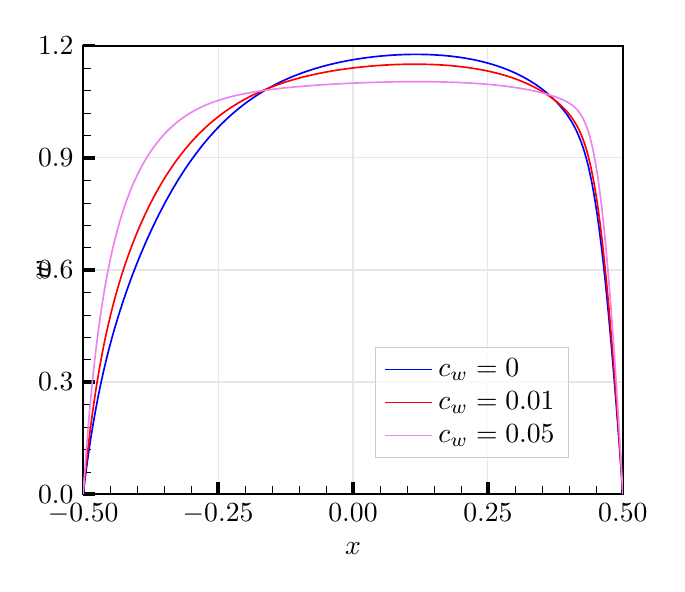
\begin{tikzpicture}

\definecolor{grey}{RGB}{128,128,128}
\definecolor{lightgrey204}{RGB}{204,204,204}
\definecolor{violet}{RGB}{238,130,238}

\begin{axis}[
legend cell align={left},
legend style={
  fill opacity=0.8,
  draw opacity=1,
  text opacity=1,
  at={(0.9,0.08)},
  anchor=south east,
  draw=lightgrey204
},
tick pos=left,
x grid style={grey!20},
xlabel={\(\displaystyle x\)},
xmajorgrids,
xmin=-0.5, xmax=0.5,
xtick style={color=black},
xtick={-0.5,-0.25,0,0.25,0.5},
xticklabels={
  \(\displaystyle {\ensuremath{-}0.50}\),
  \(\displaystyle {\ensuremath{-}0.25}\),
  \(\displaystyle {0.00}\),
  \(\displaystyle {0.25}\),
  \(\displaystyle {0.50}\)
},
y grid style={grey!20},
ylabel={\(\displaystyle w\)},
y label style={yshift=-2.5ex},
ymajorgrids,
ymin=0, ymax=1.2,
ytick style={color=black},
ytick={0,0.3,0.6,0.9,1.2},
yticklabels={
  \(\displaystyle {0.0}\),
  \(\displaystyle {0.3}\),
  \(\displaystyle {0.6}\),
  \(\displaystyle {0.9}\),
  \(\displaystyle {1.2}\)
},
minor tick num=4,
tick style={line width=1.2pt, black},
minor tick style={line width=0.15pt, black},
axis line style={line width=0.8pt, black},
]
\addplot [semithick, blue]
table {%
-0.5 0
-0.49994849945197 0.0006230607117159
-0.499794018693516 0.002488091708245
-0.499536620373079 0.0055826967515406
-0.499176408876496 0.009886405436318
-0.498713530284668 0.0153709560541192
-0.498148172314321 0.0220006871807088
-0.497480564241873 0.0297330337717139
-0.496710976810456 0.0385191202337376
-0.495839722120121 0.0483044449914014
-0.494867153501264 0.0590296416490319
-0.493793665371336 0.0706313098412411
-0.492619693074894 0.0830428937583374
-0.491345712707046 0.0961955979874534
-0.489972240920377 0.110019313999837
-0.488499834715425 0.124443543973305
-0.48692909121479 0.139398293899719
-0.485260647420981 0.154814922682823
-0.483495179958082 0.170626921792437
-0.481633404797351 0.186770615712696
-0.479676076966869 0.203185763632631
-0.477623990245336 0.219816058443311
-0.475477976840169 0.236609510911958
-0.473238907050001 0.253518721639999
-0.47090768891174 0.270501036319803
-0.468485267832324 0.287518593255239
-0.465972626205314 0.304538265785447
-0.463370783012499 0.321531513996728
-0.460680793410648 0.338474153976506
-0.457903748303608 0.355346062338618
-0.455040773899887 0.372130827244426
-0.452093031255939 0.388815364112522
-0.449061715805301 0.405389507266822
-0.445948056873795 0.421845593612104
-0.442753317180985 0.43817804747447
-0.439478792328093 0.454382979152218
-0.436125810272576 0.470457803271771
-0.432695730789584 0.486400885622159
-0.429189944920516 0.502211221495224
-0.425609874408889 0.517888150677091
-0.421956971123768 0.533431109491688
-0.418232716470968 0.548839422153745
-0.414438620792282 0.56411212982996
-0.410576222752975 0.579247857507729
-0.406647088717789 0.594244715722631
-0.402652812115718 0.609100235786137
-0.398595012793805 0.62381133480545
-0.394475336360226 0.638374308268739
-0.390295453516925 0.652784846192867
-0.386057059382078 0.667038070190022
-0.381761872802647 0.681128587487741
-0.377411635657318 0.695050559162825
-0.373008112150095 0.708797778889247
-0.368553088094842 0.722363759593927
-0.364048370191059 0.735741824741284
-0.359495785291191 0.748925201940714
-0.354897179659761 0.761907116129159
-0.350254418224633 0.774680880446013
-0.345569383820707 0.787239982657626
-0.340843976426345 0.799578165754113
-0.336080112392858 0.811689501218206
-0.331279723667337 0.82356845413255
-0.326444757009172 0.835209939260431
-0.321577173200559 0.846609367801954
-0.316678946251317 0.857762684543864
-0.311752062598348 0.868666395581421
-0.306798520300052 0.879317586820841
-0.301820328226031 0.88971393381891
-0.296819505242404 0.899853703532088
-0.291798079393078 0.909735748785119
-0.286758087077287 0.919359496252257
-0.281701572223747 0.928724928887115
-0.276630585461758 0.937832563676174
-0.271547183289587 0.946683425649516
-0.266453427240473 0.955279018992499
-0.261351383046584 0.963621296093982
-0.256243119801282 0.971712625255763
-0.251130709120015 0.979555757738553
-0.24601622430019 0.987153794701784
-0.240901739480366 0.994510154526011
-0.235789328799099 1.00162854089473
-0.230681065553797 1.00851291194236
-0.225579021359908 1.01516745068157
-0.220485265310793 1.02159653686201
-0.215401863138623 1.02780472034289
-0.210330876376634 1.0337966960179
-0.205274361523094 1.03957728028556
-0.200234369207303 1.04515138903151
-0.195212943357977 1.05052401706562
-0.19021212037435 1.0557002189469
-0.185233928300328 1.06068509112023
-0.180280386002033 1.06548375529084
-0.175353502349064 1.07010134296381
-0.170455275399822 1.07454298108358
-0.165587691591209 1.07881377871484
-0.160752724933044 1.08291881471622
-0.155952336207523 1.08686312636389
-0.151188472174036 1.09065169889162
-0.146463064779674 1.09428945591918
-0.141778030375748 1.09778125074531
-0.13713526894062 1.10113185848489
-0.13253666330919 1.1043459690317
-0.127984078409322 1.10742818082817
-0.123479360505539 1.11038299542246
-0.119024336450286 1.11321481279116
-0.114620812943063 1.1159279274037
-0.110270575797734 1.11852652500048
-0.105975389218302 1.12101468005414
-0.101736995083455 1.12339635387956
-0.097557112240155 1.12567539335516
-0.0934374358065758 1.12785553021458
-0.0893796364846631 1.12994038086605
-0.0853853598825923 1.13193344669438
-0.0814562258474062 1.13383811479888
-0.0775938278080988 1.13565765912069
-0.0737997321294127 1.13739524191134
-0.0700754774766127 1.13905391549581
-0.066422574191492 1.14063662428421
-0.0628425036798653 1.14214620698679
-0.0593367178107966 1.14358539898966
-0.0559066383278049 1.14495683485024
-0.0525536562722878 1.1462630508742
-0.0492791314193958 1.14750648773834
-0.046084391726586 1.14868949312653
-0.0429707327950797 1.14981432434902
-0.0399394173444415 1.15088315091876
-0.0369916747004938 1.15189805706103
-0.0341287002967733 1.15286104413594
-0.0313516551897324 1.1537740329567
-0.0286616655878819 1.15463886598907
-0.0260598223950666 1.15545730942049
-0.0235471807680572 1.15623105509031
-0.0211247596886407 1.15696172227458
-0.0187935415503799 1.15765085932182
-0.0165544717602116 1.15829994513813
-0.0144084583550445 1.1589103905219
-0.012356371633512 1.15948353935082
-0.0103990438030294 1.16002066962476
-0.0085372686422993 1.16052299437038
-0.0067718011794 1.16099166241383
-0.0051033573855911 1.16142775902971
-0.0035326138849561 1.16183230647475
-0.0020602076800033 1.16220626441616
-0.0006867358933344 1.16255053026352
0.0006867358933344 1.16289041304197
0.0020602076800033 1.16322593492075
0.0035326138849561 1.16358080646737
0.0051033573855911 1.16395391052467
0.0067718011794 1.16434407288205
0.0085372686422993 1.16475006562398
0.0103990438030294 1.16517061050189
0.012356371633512 1.16560438230274
0.0144084583550445 1.16605001218608
0.0165544717602116 1.16650609096303
0.0187935415503799 1.16697117229039
0.0211247596886407 1.16744377575537
0.0235471807680572 1.16792238982738
0.0260598223950666 1.16840547465502
0.0286616655878819 1.16889146468857
0.0313516551897324 1.16937877111005
0.0341287002967733 1.16986578405542
0.0369916747004938 1.17035087461585
0.0399394173444415 1.17083239660724
0.0429707327950797 1.17130868810004
0.046084391726586 1.17177807270382
0.0492791314193958 1.17223886060387
0.0525536562722878 1.1726893493495
0.0559066383278049 1.17312782439639
0.0593367178107966 1.17355255940792
0.0628425036798653 1.17396181632237
0.066422574191492 1.17435384519578
0.0700754774766127 1.17472688383168
0.0737997321294127 1.17507915721128
0.0775938278080988 1.17540887673903
0.0814562258474062 1.17571423932027
0.0853853598825923 1.1759934262886
0.0893796364846631 1.17624460220165
0.0934374358065758 1.17646591352498
0.097557112240155 1.17665548722351
0.101736995083455 1.17681142928085
0.105975389218302 1.17693182316631
0.110270575797734 1.1770147282688
0.114620812943063 1.17705817831681
0.119024336450286 1.17706017980169
0.123479360505539 1.17701871042118
0.127984078409322 1.17693171755814
0.13253666330919 1.17679711680768
0.13713526894062 1.17661279056387
0.141778030375748 1.17637658667535
0.146463064779674 1.17608631717635
0.151188472174036 1.17573975709716
0.155952336207523 1.17533464335565
0.160752724933044 1.1748686737281
0.165587691591209 1.17433950589496
0.170455275399822 1.17374475655399
0.175353502349064 1.17308200058992
0.180280386002033 1.17234877028723
0.185233928300328 1.1715425545686
0.19021212037435 1.17066079823947
0.195212943357977 1.16970090121513
0.200234369207303 1.16866021770446
0.205274361523094 1.16753605532101
0.210330876376634 1.1663256740895
0.215401863138623 1.16502628531289
0.220485265310793 1.16363505026215
0.225579021359908 1.16214907864844
0.230681065553797 1.16056542683388
0.235789328799099 1.15888109573426
0.240901739480366 1.15709302836441
0.24601622430019 1.15519810697105
0.251130709120015 1.15319314969568
0.256243119801282 1.15107490670212
0.261351383046584 1.1488400557002
0.266453427240473 1.14648519678299
0.271547183289587 1.14400684649096
0.276630585461758 1.14140143099488
0.281701572223747 1.13866527828101
0.286758087077287 1.13579460918687
0.291798079393078 1.13278552711958
0.296819505242404 1.12963400623198
0.301820328226031 1.1263358777948
0.306798520300052 1.12288681440576
0.311752062598348 1.11928231158779
0.316678946251317 1.11551766613292
0.321577173200559 1.11158795032568
0.326444757009172 1.10748798071906
0.331279723667337 1.10321227950844
0.336080112392858 1.09875502538969
0.340843976426345 1.09410998908057
0.345569383820707 1.08927044583847
0.350254418224633 1.0842290532455
0.354897179659761 1.07897767652355
0.359495785291191 1.0735071359435
0.364048370191059 1.06780684131826
0.368553088094842 1.06186426883121
0.373008112150095 1.05566422725781
0.377411635657318 1.04918785853398
0.381761872802647 1.04241132579016
0.386057059382078 1.03530416692912
0.390295453516925 1.0278273369169
0.394475336360226 1.01993102984074
0.398595012793805 1.01155245694129
0.402652812115718 1.00261385008589
0.406647088717789 0.993021041769088
0.410576222752975 0.982663022720837
0.414438620792282 0.971412871675986
0.418232716470968 0.959130375843505
0.421956971123768 0.945666507611926
0.425609874408889 0.93086970948494
0.429189944920516 0.914593688717895
0.432695730789584 0.896706182070814
0.436125810272576 0.877097957133955
0.439478792328093 0.855691216744909
0.442753317180985 0.832446580985412
0.445948056873795 0.807367951593731
0.449061715805301 0.780504783848082
0.452093031255939 0.751951580898025
0.455040773899887 0.721844720485826
0.457903748303608 0.690357000286338
0.460680793410648 0.657690483568144
0.463370783012499 0.624068348643071
0.465972626205314 0.589726455618105
0.468485267832324 0.554905289970101
0.47090768891174 0.51984280416579
0.473238907050001 0.484768529016773
0.475477976840169 0.449899141323993
0.477623990245336 0.415435531507185
0.479676076966869 0.381561269121328
0.481633404797351 0.34844228833703
0.483495179958082 0.316227540943301
0.485260647420981 0.28505036164958
0.48692909121479 0.255030274226922
0.488499834715425 0.226275012303887
0.489972240920377 0.198882541557158
0.491345712707046 0.172942934707114
0.492619693074894 0.148539968887643
0.493793665371336 0.125752380330645
0.494867153501264 0.104654722394563
0.495839722120121 0.0853178310450246
0.496710976810456 0.0678089026287389
0.497480564241873 0.0521912375262646
0.498148172314321 0.0385236948442826
0.498713530284668 0.0268599413454649
0.499176408876496 0.0172475637259045
0.499536620373079 0.0097271355206734
0.499794018693516 0.0043313160331238
0.49994849945197 0.0010840596297053
0.5 0
};
\addlegendentry{\(\displaystyle c_w=0\)}
\addplot [semithick, red]
table {%
-0.5 0
-0.49994849945197 0.0007757778852536
-0.499794018693516 0.0030975358773917
-0.499536620373079 0.0069486219633345
-0.499176408876496 0.0123015320479077
-0.498713530284668 0.0191182814872202
-0.498148172314321 0.0273509202911129
-0.497480564241873 0.0369421872383088
-0.496710976810456 0.0478262940993962
-0.495839722120121 0.0599298334749876
-0.494867153501264 0.0731727920235325
-0.493793665371336 0.0874696599977893
-0.492619693074894 0.102730609126389
-0.491345712707046 0.118862724230309
-0.489972240920377 0.135771253674271
-0.488499834715425 0.153360859343514
-0.48692909121479 0.171536828903876
-0.485260647420981 0.190206230828317
-0.483495179958082 0.209278978420165
-0.481633404797351 0.228668788167785
-0.479676076966869 0.248294006620277
-0.477623990245336 0.268078299009128
-0.475477976840169 0.287951183780768
-0.473238907050001 0.307848415202127
-0.47090768891174 0.327712208716504
-0.468485267832324 0.34749132020935
-0.465972626205314 0.367140983877831
-0.463370783012499 0.386622727595841
-0.460680793410648 0.405904078208249
-0.457903748303608 0.424958180210326
-0.455040773899887 0.443763344036314
-0.452093031255939 0.462302547823673
-0.449061715805301 0.480562908563715
-0.445948056873795 0.498535143450892
-0.442753317180985 0.516213034197251
-0.439478792328093 0.533592910193164
-0.436125810272576 0.550673158920575
-0.432695730789584 0.567453774150844
-0.429189944920516 0.583935945965428
-0.425609874408889 0.600121698294729
-0.421956971123768 0.616013574321925
-0.418232716470968 0.631614371584156
-0.414438620792282 0.646926924398889
-0.410576222752975 0.661953932699085
-0.406647088717789 0.67669783319185
-0.402652812115718 0.691160710217018
-0.398595012793805 0.705344241380807
-0.394475336360226 0.719249674480638
-0.390295453516925 0.73287783061989
-0.386057059382078 0.746229129788723
-0.381761872802647 0.759303634083859
-0.377411635657318 0.772101105015288
-0.373008112150095 0.784621070628894
-0.368553088094842 0.796862899325056
-0.364048370191059 0.808825876815519
-0.359495785291191 0.820509283684452
-0.354897179659761 0.831912470785911
-0.350254418224633 0.843034930607544
-0.345569383820707 0.853876362641059
-0.340843976426345 0.864436731573976
-0.336080112392858 0.874716317120758
-0.331279723667337 0.884715754963282
-0.326444757009172 0.894436068321177
-0.321577173200559 0.903878690202441
-0.316678946251317 0.913045476444744
-0.311752062598348 0.92193871006397
-0.306798520300052 0.930561097467348
-0.301820328226031 0.938915757373584
-0.296819505242404 0.94700620328583
-0.291798079393078 0.954836320534094
-0.286758087077287 0.962410338862455
-0.281701572223747 0.969732801612608
-0.276630585461758 0.97680853246709
-0.271547183289587 0.983642600714524
-0.266453427240473 0.990240285882209
-0.261351383046584 0.996607042525449
-0.256243119801282 1.00274846582992
-0.251130709120015 1.00867025859752
-0.24601622430019 1.01437820005399
-0.240901739480366 1.01987811682312
-0.235789328799099 1.02517585629321
-0.230681065553797 1.03027726251789
-0.225579021359908 1.03518815469806
-0.220485265310793 1.0399143082258
-0.215401863138623 1.04446143820586
-0.210330876376634 1.04883518532668
-0.205274361523094 1.05304110391563
-0.200234369207303 1.05708465199196
-0.195212943357977 1.06097118311722
-0.19021212037435 1.06470593984046
-0.185233928300328 1.06829404853868
-0.180280386002033 1.0717405154637
-0.175353502349064 1.07505022381979
-0.170455275399822 1.07822793171389
-0.165587691591209 1.08127827083874
-0.160752724933044 1.08420574576859
-0.155952336207523 1.0870147337645
-0.151188472174036 1.08970948500488
-0.146463064779674 1.09229412317252
-0.141778030375748 1.09477264634266
-0.13713526894062 1.0971489281291
-0.13253666330919 1.09942671905489
-0.127984078409322 1.10160964812186
-0.123479360505539 1.10370122455923
-0.119024336450286 1.10570483973541
-0.114620812943063 1.1076237692203
-0.110270575797734 1.10946117498674
-0.105975389218302 1.11122010774046
-0.101736995083455 1.11290350936806
-0.097557112240155 1.11451421549161
-0.0934374358065758 1.11605495811813
-0.0893796364846631 1.11752836837106
-0.0853853598825923 1.11893697928959
-0.0814562258474062 1.12028322868134
-0.0775938278080988 1.12156946201299
-0.0737997321294127 1.12279793532252
-0.0700754774766127 1.12397081813692
-0.066422574191492 1.12509019637916
-0.0628425036798653 1.12615807524829
-0.0593367178107966 1.12717638205673
-0.0559066383278049 1.12814696901006
-0.0525536562722878 1.12907161591507
-0.0492791314193958 1.12995203280312
-0.046084391726586 1.13078986245672
-0.0429707327950797 1.13158668282884
-0.0399394173444415 1.13234400934582
-0.0369916747004938 1.133063297086
-0.0341287002967733 1.13374594282762
-0.0313516551897324 1.13439328696152
-0.0286616655878819 1.13500661526484
-0.0260598223950666 1.13558716053397
-0.0235471807680572 1.13613610407621
-0.0211247596886407 1.13665457706078
-0.0187935415503799 1.13714366173119
-0.0165544717602116 1.13760439248226
-0.0144084583550445 1.13803775680581
-0.012356371633512 1.1384446961103
-0.0103990438030294 1.13882610642061
-0.0085372686422993 1.13918283896462
-0.0067718011794 1.13951570065425
-0.0051033573855911 1.13982545446884
-0.0035326138849561 1.14011281974945
-0.0020602076800033 1.14037847241295
-0.0006867358933344 1.14062304509415
0.0006867358933344 1.14086451485416
0.0020602076800033 1.14110289591247
0.0035326138849561 1.14135503342147
0.0051033573855911 1.14162013339671
0.0067718011794 1.14189736055346
0.0085372686422993 1.14218584054098
0.0103990438030294 1.1424846621861
0.012356371633512 1.14279287972777
0.0144084583550445 1.14310951502329
0.0165544717602116 1.143433559708
0.0187935415503799 1.14376397729046
0.0211247596886407 1.14409970516644
0.0235471807680572 1.14443965653574
0.0260598223950666 1.14478272220749
0.0286616655878819 1.14512777228052
0.0313516551897324 1.14547365768732
0.0341287002967733 1.14581921159125
0.0369916747004938 1.14616325062859
0.0399394173444415 1.14650457598863
0.0429707327950797 1.14684197432691
0.046084391726586 1.14717421850807
0.0492791314193958 1.14750006817718
0.0525536562722878 1.14781827015975
0.0559066383278049 1.14812755869242
0.0593367178107966 1.14842665548812
0.0628425036798653 1.14871426964065
0.066422574191492 1.14898909737596
0.0700754774766127 1.1492498216578
0.0737997321294127 1.14949511165744
0.0775938278080988 1.14972362209783
0.0814562258474062 1.1499339924836
0.0853853598825923 1.15012484622944
0.0893796364846631 1.15029478969936
0.0934374358065758 1.15044241117064
0.097557112240155 1.15056627973567
0.101736995083455 1.1506649441557
0.105975389218302 1.15073693168001
0.110270575797734 1.15078074684377
0.114620812943063 1.15079487025737
0.119024336450286 1.15077775739944
0.123479360505539 1.15072783742498
0.127984078409322 1.1506435119986
0.13253666330919 1.15052315416212
0.13713526894062 1.15036510724389
0.141778030375748 1.15016768381632
0.146463064779674 1.14992916470569
0.151188472174036 1.14964779805688
0.155952336207523 1.14932179845392
0.160752724933044 1.14894934609453
0.165587691591209 1.14852858601538
0.170455275399822 1.14805762736221
0.175353502349064 1.14753454269651
0.180280386002033 1.14695736732862
0.185233928300328 1.14632409866444
0.19021212037435 1.14563269555059
0.195212943357977 1.14488107760057
0.200234369207303 1.14406712448218
0.205274361523094 1.1431886751441
0.210330876376634 1.14224352695729
0.215401863138623 1.14122943474457
0.220485265310793 1.14014410966927
0.225579021359908 1.13898521795175
0.230681065553797 1.13775037937991
0.235789328799099 1.13643716557725
0.240901739480366 1.13504309798963
0.24601622430019 1.13356564554733
0.251130709120015 1.13200222195673
0.256243119801282 1.13035018256936
0.261351383046584 1.1286068207733
0.266453427240473 1.12676936384116
0.271547183289587 1.12483496816358
0.276630585461758 1.1228007137821
0.281701572223747 1.12066359812585
0.286758087077287 1.11842052883003
0.291798079393078 1.11606831549925
0.296819505242404 1.11360366023392
0.301820328226031 1.111023146706
0.306798520300052 1.1083232274916
0.311752062598348 1.10550020929078
0.316678946251317 1.10255023549885
0.321577173200559 1.09946926539118
0.326444757009172 1.09625304876567
0.331279723667337 1.09289709428532
0.336080112392858 1.0893966286415
0.340843976426345 1.08574654193362
0.345569383820707 1.0819413117531
0.350254418224633 1.07797489415551
0.354897179659761 1.07384056325103
0.359495785291191 1.06953067256249
0.364048370191059 1.06503630036481
0.368553088094842 1.06034672938717
0.373008112150095 1.05544870036291
0.377411635657318 1.05032537349675
0.381761872802647 1.04495493683713
0.386057059382078 1.03930882292984
0.390295453516925 1.03334953975712
0.394475336360226 1.02702819254297
0.398595012793805 1.02028186551683
0.402652812115718 1.01303113819463
0.406647088717789 1.00517810933324
0.410576222752975 0.99660537108339
0.414438620792282 0.987176388416998
0.418232716470968 0.976737676893036
0.421956971123768 0.965123024242727
0.425609874408889 0.952159780577041
0.429189944920516 0.937676971550437
0.432695730789584 0.921514715586795
0.436125810272576 0.903534193209863
0.439478792328093 0.883627275595879
0.442753317180985 0.861724892728967
0.445948056873795 0.837803328257266
0.449061715805301 0.811887841223864
0.452093031255939 0.784053313718139
0.455040773899887 0.754421942997867
0.457903748303608 0.723158307080607
0.460680793410648 0.690462367638541
0.463370783012499 0.656561132912551
0.465972626205314 0.621699744523838
0.468485267832324 0.586132718709789
0.47090768891174 0.550115944106001
0.473238907050001 0.513899887712761
0.475477976840169 0.477724266337762
0.477623990245336 0.44181428320002
0.479676076966869 0.406378366188694
0.481633404797351 0.371607251603568
0.483495179958082 0.337674167389168
0.485260647420981 0.304735855768481
0.48692909121479 0.272934150091542
0.488499834715425 0.242397861561063
0.489972240920377 0.213244741229605
0.491345712707046 0.185583347864016
0.492619693074894 0.159514670741837
0.493793665371336 0.135133425329322
0.494867153501264 0.112528953099678
0.495839722120121 0.0917857197995931
0.496710976810456 0.072983409890574
0.497480564241873 0.0561966684720967
0.498148172314321 0.0414945354120023
0.498713530284668 0.0289396580168703
0.499176408876496 0.0185873551047846
0.499536620373079 0.0104846294526914
0.499794018693516 0.0046692115536309
0.49994849945197 0.0011687188331739
0.5 0
};
\addlegendentry{\(\displaystyle c_w=0.01\)}
\addplot [semithick, violet]
table {%
-0.5 0
-0.49994849945197 0.0011129310193128
-0.499794018693516 0.0044426873079972
-0.499536620373079 0.0099622779927262
-0.499176408876496 0.017627115797779
-0.498713530284668 0.0273756110692171
-0.498148172314321 0.0391299982528427
-0.497480564241873 0.0527973892060262
-0.496710976810456 0.0682710416223167
-0.495839722120121 0.0854318330618087
-0.494867153501264 0.104149913936509
-0.493793665371336 0.124286523900429
-0.492619693074894 0.145695929131473
-0.491345712707046 0.168227454728658
-0.489972240920377 0.191727557788402
-0.488499834715425 0.216041906535465
-0.48692909121479 0.241017405816465
-0.485260647420981 0.266504132246446
-0.483495179958082 0.292357123152605
-0.481633404797351 0.31843798925447
-0.479676076966869 0.344616307754896
-0.477623990245336 0.370770779540333
-0.475477976840169 0.396790125273078
-0.473238907050001 0.422573721328792
-0.47090768891174 0.448031970070933
-0.468485267832324 0.473086422378523
-0.465972626205314 0.497669664537688
-0.463370783012499 0.521725000704961
-0.460680793410648 0.545205955438598
-0.457903748303608 0.568075634548772
-0.455040773899887 0.590305974057934
-0.452093031255939 0.611876915523692
-0.449061715805301 0.63277553602699
-0.445948056873795 0.652995165427266
-0.442753317180985 0.672534513087165
-0.439478792328093 0.691396827993792
-0.436125810272576 0.709589106484046
-0.432695730789584 0.727121362313499
-0.429189944920516 0.744005965528354
-0.425609874408889 0.760257056850497
-0.421956971123768 0.775890037763736
-0.418232716470968 0.790921136932811
-0.414438620792282 0.805367048810771
-0.410576222752975 0.819244641090898
-0.406647088717789 0.832570724409535
-0.402652812115718 0.845361878833628
-0.398595012793805 0.857634329625071
-0.394475336360226 0.869403866103048
-0.390295453516925 0.880685796260492
-0.386057059382078 0.891494931182509
-0.381761872802647 0.901845592738709
-0.377411635657318 0.91175163936154
-0.373008112150095 0.921226504522025
-0.368553088094842 0.930283243732006
-0.364048370191059 0.938934585923393
-0.359495785291191 0.947192986118259
-0.354897179659761 0.95507067644553
-0.350254418224633 0.962579713459805
-0.345569383820707 0.969732019912982
-0.340843976426345 0.976539419867729
-0.336080112392858 0.983013666245098
-0.331279723667337 0.989166460482183
-0.326444757009172 0.995009464154023
-0.321577173200559 1.00055430285273
-0.316678946251317 1.00581256274796
-0.311752062598348 1.01079578055632
-0.306798520300052 1.01551542771859
-0.301820328226031 1.0199828897652
-0.296819505242404 1.02420944185768
-0.291798079393078 1.0282062215705
-0.286758087077287 1.03198419992603
-0.281701572223747 1.03555415168945
-0.276630585461758 1.03892662583122
-0.271547183289587 1.04211191699777
-0.266453427240473 1.04512003870506
-0.261351383046584 1.04796069886699
-0.256243119801282 1.05064327813287
-0.251130709120015 1.05317681139463
-0.24601622430019 1.0555699726936
-0.240901739480366 1.05783106364954
-0.235789328799099 1.05996800542362
-0.230681065553797 1.06198833414081
-0.225579021359908 1.0638991996139
-0.220485265310793 1.06570736715122
-0.215401863138623 1.06741922217871
-0.210330876376634 1.0690407773738
-0.205274361523094 1.07057768198671
-0.200234369207303 1.07203523301516
-0.195212943357977 1.07341838790075
-0.19021212037435 1.07473177842488
-0.185233928300328 1.0759797254989
-0.180280386002033 1.0771662545674
-0.175353502349064 1.0782951113687
-0.170455275399822 1.07936977782569
-0.165587691591209 1.08039348787108
-0.160752724933044 1.08136924303958
-0.155952336207523 1.08229982768887
-0.151188472174036 1.08318782373853
-0.146463064779674 1.08403562484124
-0.141778030375748 1.08484544992246
-0.13713526894062 1.08561935604529
-0.13253666330919 1.08635925057425
-0.127984078409322 1.08706690262647
-0.123479360505539 1.08774395381046
-0.119024336450286 1.08839192826294
-0.114620812943063 1.08901224200126
-0.110270575797734 1.08960621161562
-0.105975389218302 1.09017506232822
-0.101736995083455 1.09071993545092
-0.097557112240155 1.09124189527307
-0.0934374358065758 1.09174193541283
-0.0893796364846631 1.09222098466534
-0.0853853598825923 1.09267991237993
-0.0814562258474062 1.09311953339773
-0.0775938278080988 1.09354061258058
-0.0737997321294127 1.09394386895883
-0.0700754774766127 1.09432997952587
-0.066422574191492 1.09469958270418
-0.0628425036798653 1.09505328150678
-0.0593367178107966 1.09539164641558
-0.0559066383278049 1.0957152179972
-0.0525536562722878 1.096024509275
-0.0492791314193958 1.09632000787468
-0.046084391726586 1.09660217795937
-0.0429707327950797 1.09687146196928
-0.0399394173444415 1.09712828217958
-0.0369916747004938 1.09737304208938
-0.0341287002967733 1.09760612765369
-0.0313516551897324 1.09782790836976
-0.0286616655878819 1.09803873822799
-0.0260598223950666 1.09823895653764
-0.0235471807680572 1.09842888863638
-0.0211247596886407 1.09860884649294
-0.0187935415503799 1.09877912921112
-0.0165544717602116 1.09894002344328
-0.0144084583550445 1.09909180372138
-0.012356371633512 1.09923473271286
-0.0103990438030294 1.09936906140863
-0.0085372686422993 1.09949502925038
-0.0067718011794 1.09961286420371
-0.0051033573855911 1.09972278278395
-0.0035326138849561 1.0998249900407
-0.0020602076800033 1.0999196795074
-0.0006867358933344 1.10000703312212
0.0006867358933344 1.1000934495064
0.0020602076800033 1.1001789308364
0.0035326138849561 1.10026953338799
0.0051033573855911 1.10036500752616
0.0067718011794 1.10046508946354
0.0085372686422993 1.10056950173517
0.0103990438030294 1.10067795366527
0.012356371633512 1.10079014182076
0.0144084583550445 1.10090575044649
0.0165544717602116 1.10102445187807
0.0187935415503799 1.10114590692781
0.0211247596886407 1.10126976523997
0.0235471807680572 1.1013956656119
0.0260598223950666 1.10152323627807
0.0286616655878819 1.10165209515437
0.0313516551897324 1.10178185004074
0.0341287002967733 1.10191209878024
0.0369916747004938 1.10204242937374
0.0399394173444415 1.10217242004919
0.0429707327950797 1.10230163928546
0.046084391726586 1.10242964579091
0.0492791314193958 1.10255598843722
0.0525536562722878 1.10268020614972
0.0559066383278049 1.10280182775565
0.0593367178107966 1.10292037179187
0.0628425036798653 1.10303534627453
0.066422574191492 1.10314624843283
0.0700754774766127 1.1032525644098
0.0737997321294127 1.10335376893292
0.0775938278080988 1.10344932495795
0.0814562258474062 1.10353868328901
0.0853853598825923 1.10362128217887
0.0893796364846631 1.10369654691242
0.0934374358065758 1.10376388937782
0.097557112240155 1.10382270762825
0.101736995083455 1.10387238543862
0.105975389218302 1.10391229186067
0.110270575797734 1.10394178077986
0.114620812943063 1.1039601904779
0.119024336450286 1.10396684320402
0.123479360505539 1.1039610447579
0.127984078409322 1.10394208408753
0.13253666330919 1.10390923290396
0.13713526894062 1.1038617453153
0.141778030375748 1.10379885748162
0.146463064779674 1.10371978729189
0.151188472174036 1.10362373406343
0.155952336207523 1.10350987826428
0.160752724933044 1.10337738125734
0.165587691591209 1.10322538506545
0.170455275399822 1.10305301215495
0.175353502349064 1.10285936523484
0.180280386002033 1.10264352706794
0.185233928300328 1.10240456028952
0.19021212037435 1.10214150722732
0.195212943357977 1.10185338971688
0.200234369207303 1.10153920890475
0.205274361523094 1.10119794503044
0.210330876376634 1.10082855717841
0.215401863138623 1.10042998298903
0.220485265310793 1.10000113831648
0.225579021359908 1.09954091682153
0.230681065553797 1.09904818948426
0.235789328799099 1.09852180402204
0.240901739480366 1.09796058419552
0.24601622430019 1.09736332898407
0.251130709120015 1.0967288116107
0.256243119801282 1.09605577839293
0.261351383046584 1.09534294739593
0.266453427240473 1.0945890068577
0.271547183289587 1.09379261335488
0.276630585461758 1.09295238967028
0.281701572223747 1.09206692231952
0.286758087077287 1.0911347586819
0.291798079393078 1.09015440367355
0.296819505242404 1.08912431588172
0.301820328226031 1.08804290306122
0.306798520300052 1.08690851685566
0.311752062598348 1.08571944656007
0.316678946251317 1.08447391163985
0.321577173200559 1.08317005256814
0.326444757009172 1.08180591922574
0.331279723667337 1.08037945556486
0.336080112392858 1.07888847820647
0.340843976426345 1.07733064487953
0.345569383820707 1.07570340556975
0.350254418224633 1.07400392441074
0.354897179659761 1.07222895290044
0.359495785291191 1.07037462447784
0.364048370191059 1.06843612649418
0.368553088094842 1.06640718906409
0.373008112150095 1.06427931323529
0.377411635657318 1.06204064793504
0.381761872802647 1.0596744225156
0.386057059382078 1.05715685797803
0.390295453516925 1.05445452303912
0.394475336360226 1.0515211773078
0.398595012793805 1.04829425238878
0.402652812115718 1.04469125442917
0.406647088717789 1.04060650859757
0.410576222752975 1.03590877981789
0.414438620792282 1.03044036110701
0.418232716470968 1.02401819261406
0.421956971123768 1.0164374415885
0.425609874408889 1.00747773920931
0.429189944920516 0.99691195647299
0.432695730789584 0.984517056139318
0.436125810272576 0.970086235414178
0.439478792328093 0.953441338141538
0.442753317180985 0.934444406377461
0.445948056873795 0.913007290274683
0.449061715805301 0.889098427876057
0.452093031255939 0.862746222259418
0.455040773899887 0.834038816468322
0.457903748303608 0.803120454145563
0.460680793410648 0.770184938833289
0.463370783012499 0.735466950296029
0.465972626205314 0.699232090929717
0.468485267832324 0.661766552242945
0.47090768891174 0.623367188660345
0.473238907050001 0.584332636207338
0.475477976840169 0.544955900475522
0.477623990245336 0.505518648422139
0.479676076966869 0.466287235754602
0.481633404797351 0.427510369507302
0.483495179958082 0.38941817844534
0.485260647420981 0.352222421356758
0.48692909121479 0.316117515444255
0.488499834715425 0.281282096340535
0.489972240920377 0.247880823398808
0.491345712707046 0.216066211387716
0.492619693074894 0.185980290246684
0.493793665371336 0.157755972900998
0.494867153501264 0.131518029869598
0.495839722120121 0.107383643687388
0.496710976810456 0.0854625246943507
0.497480564241873 0.0658566338109533
0.498148172314321 0.0486595549541192
0.498713530284668 0.0339556099386371
0.499176408876496 0.0218187969970529
0.499536620373079 0.0123116634153077
0.499794018693516 0.0054842087221517
0.49994849945197 0.0013729169241406
0.5 0
};
\addlegendentry{\(\displaystyle c_w=0.05\)}
\end{axis}
\end{tikzpicture}
}
		\label{fig:phv}}
\end{figure}

\begin{lstlisting}[numbers=left,frame=single,language=Python]
\begin{tikzpicture}

\definecolor{grey}{RGB}{128,128,128}
\definecolor{lightgrey204}{RGB}{204,204,204}
\definecolor{violet}{RGB}{238,130,238}

\begin{axis}[
legend cell align={left},
legend style={
fill opacity=0.8,
draw opacity=1,
text opacity=1,
at={(0.9,0.08)},
anchor=south east,
draw=lightgrey204
},
tick pos=left,
x grid style={grey!20},
xlabel={\(\displaystyle x\)},
xmajorgrids,
xmin=-0.5, xmax=0.5,
xtick style={color=black},
xtick={-0.5,-0.25,0,0.25,0.5},
xticklabels={
\(\displaystyle {\ensuremath{-}0.50}\),
\(\displaystyle {\ensuremath{-}0.25}\),
\(\displaystyle {0.00}\),
\(\displaystyle {0.25}\),
\(\displaystyle {0.50}\)
},
y grid style={grey!20},
ylabel={\(\displaystyle w\)},
y label style={yshift=-2.5ex},
ymajorgrids,
ymin=0, ymax=1.2,
ytick style={color=black},
ytick={0,0.3,0.6,0.9,1.2},
yticklabels={
\(\displaystyle {0.0}\),
\(\displaystyle {0.3}\),
\(\displaystyle {0.6}\),
\(\displaystyle {0.9}\),
\(\displaystyle {1.2}\)
},
minor tick num=4,
tick style={line width=1.2pt, black},
minor tick style={line width=0.15pt, black},
axis line style={line width=0.8pt, black},
]
\addplot [semithick, blue]
table {%
...
};
\addlegendentry{\(\displaystyle c_w=0.05\)}
\end{axis}
\end{tikzpicture}
\end{lstlisting}

其中第33,45,46,47,48行都是后来手动加上去的,第13行position也有有调整;33行平移轴线位置,45行设置副刻度数量,46-47设置主副刻度线粗细,48设置轴线粗细;\par

在文中的插入只需用\verb input 命令对外部的tex文件进行插入即可,例如上文中对图片的插入:\par

\begin{lstlisting}[numbers=left,frame=single,language=Python]
\begin{figure}[htbp]
  \centering{
  \raisebox{33ex}{\makebox[0pt][l]{(a)}}
  \scalebox{0.78}{% This file was created with tikzplotlib v0.10.1.post12.
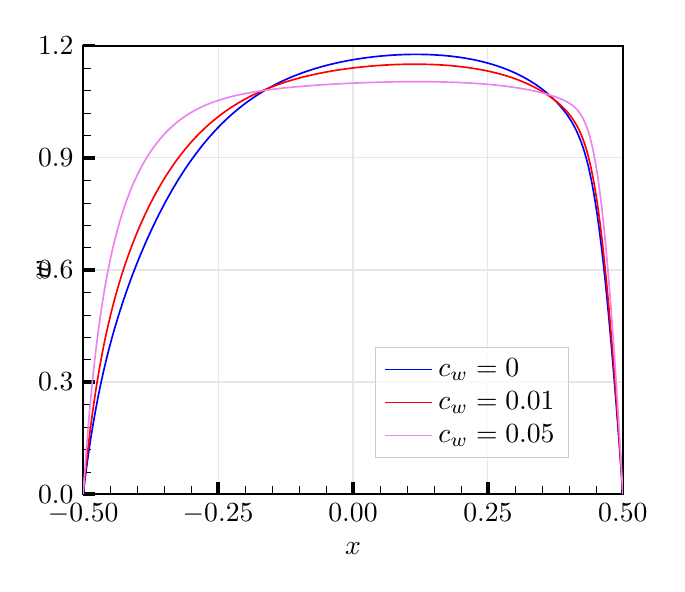
\begin{tikzpicture}

\definecolor{grey}{RGB}{128,128,128}
\definecolor{lightgrey204}{RGB}{204,204,204}
\definecolor{violet}{RGB}{238,130,238}

\begin{axis}[
legend cell align={left},
legend style={
  fill opacity=0.8,
  draw opacity=1,
  text opacity=1,
  at={(0.9,0.08)},
  anchor=south east,
  draw=lightgrey204
},
tick pos=left,
x grid style={grey!20},
xlabel={\(\displaystyle x\)},
xmajorgrids,
xmin=-0.5, xmax=0.5,
xtick style={color=black},
xtick={-0.5,-0.25,0,0.25,0.5},
xticklabels={
  \(\displaystyle {\ensuremath{-}0.50}\),
  \(\displaystyle {\ensuremath{-}0.25}\),
  \(\displaystyle {0.00}\),
  \(\displaystyle {0.25}\),
  \(\displaystyle {0.50}\)
},
y grid style={grey!20},
ylabel={\(\displaystyle w\)},
y label style={yshift=-2.5ex},
ymajorgrids,
ymin=0, ymax=1.2,
ytick style={color=black},
ytick={0,0.3,0.6,0.9,1.2},
yticklabels={
  \(\displaystyle {0.0}\),
  \(\displaystyle {0.3}\),
  \(\displaystyle {0.6}\),
  \(\displaystyle {0.9}\),
  \(\displaystyle {1.2}\)
},
minor tick num=4,
tick style={line width=1.2pt, black},
minor tick style={line width=0.15pt, black},
axis line style={line width=0.8pt, black},
]
\addplot [semithick, blue]
table {%
-0.5 0
-0.49994849945197 0.0006230607117159
-0.499794018693516 0.002488091708245
-0.499536620373079 0.0055826967515406
-0.499176408876496 0.009886405436318
-0.498713530284668 0.0153709560541192
-0.498148172314321 0.0220006871807088
-0.497480564241873 0.0297330337717139
-0.496710976810456 0.0385191202337376
-0.495839722120121 0.0483044449914014
-0.494867153501264 0.0590296416490319
-0.493793665371336 0.0706313098412411
-0.492619693074894 0.0830428937583374
-0.491345712707046 0.0961955979874534
-0.489972240920377 0.110019313999837
-0.488499834715425 0.124443543973305
-0.48692909121479 0.139398293899719
-0.485260647420981 0.154814922682823
-0.483495179958082 0.170626921792437
-0.481633404797351 0.186770615712696
-0.479676076966869 0.203185763632631
-0.477623990245336 0.219816058443311
-0.475477976840169 0.236609510911958
-0.473238907050001 0.253518721639999
-0.47090768891174 0.270501036319803
-0.468485267832324 0.287518593255239
-0.465972626205314 0.304538265785447
-0.463370783012499 0.321531513996728
-0.460680793410648 0.338474153976506
-0.457903748303608 0.355346062338618
-0.455040773899887 0.372130827244426
-0.452093031255939 0.388815364112522
-0.449061715805301 0.405389507266822
-0.445948056873795 0.421845593612104
-0.442753317180985 0.43817804747447
-0.439478792328093 0.454382979152218
-0.436125810272576 0.470457803271771
-0.432695730789584 0.486400885622159
-0.429189944920516 0.502211221495224
-0.425609874408889 0.517888150677091
-0.421956971123768 0.533431109491688
-0.418232716470968 0.548839422153745
-0.414438620792282 0.56411212982996
-0.410576222752975 0.579247857507729
-0.406647088717789 0.594244715722631
-0.402652812115718 0.609100235786137
-0.398595012793805 0.62381133480545
-0.394475336360226 0.638374308268739
-0.390295453516925 0.652784846192867
-0.386057059382078 0.667038070190022
-0.381761872802647 0.681128587487741
-0.377411635657318 0.695050559162825
-0.373008112150095 0.708797778889247
-0.368553088094842 0.722363759593927
-0.364048370191059 0.735741824741284
-0.359495785291191 0.748925201940714
-0.354897179659761 0.761907116129159
-0.350254418224633 0.774680880446013
-0.345569383820707 0.787239982657626
-0.340843976426345 0.799578165754113
-0.336080112392858 0.811689501218206
-0.331279723667337 0.82356845413255
-0.326444757009172 0.835209939260431
-0.321577173200559 0.846609367801954
-0.316678946251317 0.857762684543864
-0.311752062598348 0.868666395581421
-0.306798520300052 0.879317586820841
-0.301820328226031 0.88971393381891
-0.296819505242404 0.899853703532088
-0.291798079393078 0.909735748785119
-0.286758087077287 0.919359496252257
-0.281701572223747 0.928724928887115
-0.276630585461758 0.937832563676174
-0.271547183289587 0.946683425649516
-0.266453427240473 0.955279018992499
-0.261351383046584 0.963621296093982
-0.256243119801282 0.971712625255763
-0.251130709120015 0.979555757738553
-0.24601622430019 0.987153794701784
-0.240901739480366 0.994510154526011
-0.235789328799099 1.00162854089473
-0.230681065553797 1.00851291194236
-0.225579021359908 1.01516745068157
-0.220485265310793 1.02159653686201
-0.215401863138623 1.02780472034289
-0.210330876376634 1.0337966960179
-0.205274361523094 1.03957728028556
-0.200234369207303 1.04515138903151
-0.195212943357977 1.05052401706562
-0.19021212037435 1.0557002189469
-0.185233928300328 1.06068509112023
-0.180280386002033 1.06548375529084
-0.175353502349064 1.07010134296381
-0.170455275399822 1.07454298108358
-0.165587691591209 1.07881377871484
-0.160752724933044 1.08291881471622
-0.155952336207523 1.08686312636389
-0.151188472174036 1.09065169889162
-0.146463064779674 1.09428945591918
-0.141778030375748 1.09778125074531
-0.13713526894062 1.10113185848489
-0.13253666330919 1.1043459690317
-0.127984078409322 1.10742818082817
-0.123479360505539 1.11038299542246
-0.119024336450286 1.11321481279116
-0.114620812943063 1.1159279274037
-0.110270575797734 1.11852652500048
-0.105975389218302 1.12101468005414
-0.101736995083455 1.12339635387956
-0.097557112240155 1.12567539335516
-0.0934374358065758 1.12785553021458
-0.0893796364846631 1.12994038086605
-0.0853853598825923 1.13193344669438
-0.0814562258474062 1.13383811479888
-0.0775938278080988 1.13565765912069
-0.0737997321294127 1.13739524191134
-0.0700754774766127 1.13905391549581
-0.066422574191492 1.14063662428421
-0.0628425036798653 1.14214620698679
-0.0593367178107966 1.14358539898966
-0.0559066383278049 1.14495683485024
-0.0525536562722878 1.1462630508742
-0.0492791314193958 1.14750648773834
-0.046084391726586 1.14868949312653
-0.0429707327950797 1.14981432434902
-0.0399394173444415 1.15088315091876
-0.0369916747004938 1.15189805706103
-0.0341287002967733 1.15286104413594
-0.0313516551897324 1.1537740329567
-0.0286616655878819 1.15463886598907
-0.0260598223950666 1.15545730942049
-0.0235471807680572 1.15623105509031
-0.0211247596886407 1.15696172227458
-0.0187935415503799 1.15765085932182
-0.0165544717602116 1.15829994513813
-0.0144084583550445 1.1589103905219
-0.012356371633512 1.15948353935082
-0.0103990438030294 1.16002066962476
-0.0085372686422993 1.16052299437038
-0.0067718011794 1.16099166241383
-0.0051033573855911 1.16142775902971
-0.0035326138849561 1.16183230647475
-0.0020602076800033 1.16220626441616
-0.0006867358933344 1.16255053026352
0.0006867358933344 1.16289041304197
0.0020602076800033 1.16322593492075
0.0035326138849561 1.16358080646737
0.0051033573855911 1.16395391052467
0.0067718011794 1.16434407288205
0.0085372686422993 1.16475006562398
0.0103990438030294 1.16517061050189
0.012356371633512 1.16560438230274
0.0144084583550445 1.16605001218608
0.0165544717602116 1.16650609096303
0.0187935415503799 1.16697117229039
0.0211247596886407 1.16744377575537
0.0235471807680572 1.16792238982738
0.0260598223950666 1.16840547465502
0.0286616655878819 1.16889146468857
0.0313516551897324 1.16937877111005
0.0341287002967733 1.16986578405542
0.0369916747004938 1.17035087461585
0.0399394173444415 1.17083239660724
0.0429707327950797 1.17130868810004
0.046084391726586 1.17177807270382
0.0492791314193958 1.17223886060387
0.0525536562722878 1.1726893493495
0.0559066383278049 1.17312782439639
0.0593367178107966 1.17355255940792
0.0628425036798653 1.17396181632237
0.066422574191492 1.17435384519578
0.0700754774766127 1.17472688383168
0.0737997321294127 1.17507915721128
0.0775938278080988 1.17540887673903
0.0814562258474062 1.17571423932027
0.0853853598825923 1.1759934262886
0.0893796364846631 1.17624460220165
0.0934374358065758 1.17646591352498
0.097557112240155 1.17665548722351
0.101736995083455 1.17681142928085
0.105975389218302 1.17693182316631
0.110270575797734 1.1770147282688
0.114620812943063 1.17705817831681
0.119024336450286 1.17706017980169
0.123479360505539 1.17701871042118
0.127984078409322 1.17693171755814
0.13253666330919 1.17679711680768
0.13713526894062 1.17661279056387
0.141778030375748 1.17637658667535
0.146463064779674 1.17608631717635
0.151188472174036 1.17573975709716
0.155952336207523 1.17533464335565
0.160752724933044 1.1748686737281
0.165587691591209 1.17433950589496
0.170455275399822 1.17374475655399
0.175353502349064 1.17308200058992
0.180280386002033 1.17234877028723
0.185233928300328 1.1715425545686
0.19021212037435 1.17066079823947
0.195212943357977 1.16970090121513
0.200234369207303 1.16866021770446
0.205274361523094 1.16753605532101
0.210330876376634 1.1663256740895
0.215401863138623 1.16502628531289
0.220485265310793 1.16363505026215
0.225579021359908 1.16214907864844
0.230681065553797 1.16056542683388
0.235789328799099 1.15888109573426
0.240901739480366 1.15709302836441
0.24601622430019 1.15519810697105
0.251130709120015 1.15319314969568
0.256243119801282 1.15107490670212
0.261351383046584 1.1488400557002
0.266453427240473 1.14648519678299
0.271547183289587 1.14400684649096
0.276630585461758 1.14140143099488
0.281701572223747 1.13866527828101
0.286758087077287 1.13579460918687
0.291798079393078 1.13278552711958
0.296819505242404 1.12963400623198
0.301820328226031 1.1263358777948
0.306798520300052 1.12288681440576
0.311752062598348 1.11928231158779
0.316678946251317 1.11551766613292
0.321577173200559 1.11158795032568
0.326444757009172 1.10748798071906
0.331279723667337 1.10321227950844
0.336080112392858 1.09875502538969
0.340843976426345 1.09410998908057
0.345569383820707 1.08927044583847
0.350254418224633 1.0842290532455
0.354897179659761 1.07897767652355
0.359495785291191 1.0735071359435
0.364048370191059 1.06780684131826
0.368553088094842 1.06186426883121
0.373008112150095 1.05566422725781
0.377411635657318 1.04918785853398
0.381761872802647 1.04241132579016
0.386057059382078 1.03530416692912
0.390295453516925 1.0278273369169
0.394475336360226 1.01993102984074
0.398595012793805 1.01155245694129
0.402652812115718 1.00261385008589
0.406647088717789 0.993021041769088
0.410576222752975 0.982663022720837
0.414438620792282 0.971412871675986
0.418232716470968 0.959130375843505
0.421956971123768 0.945666507611926
0.425609874408889 0.93086970948494
0.429189944920516 0.914593688717895
0.432695730789584 0.896706182070814
0.436125810272576 0.877097957133955
0.439478792328093 0.855691216744909
0.442753317180985 0.832446580985412
0.445948056873795 0.807367951593731
0.449061715805301 0.780504783848082
0.452093031255939 0.751951580898025
0.455040773899887 0.721844720485826
0.457903748303608 0.690357000286338
0.460680793410648 0.657690483568144
0.463370783012499 0.624068348643071
0.465972626205314 0.589726455618105
0.468485267832324 0.554905289970101
0.47090768891174 0.51984280416579
0.473238907050001 0.484768529016773
0.475477976840169 0.449899141323993
0.477623990245336 0.415435531507185
0.479676076966869 0.381561269121328
0.481633404797351 0.34844228833703
0.483495179958082 0.316227540943301
0.485260647420981 0.28505036164958
0.48692909121479 0.255030274226922
0.488499834715425 0.226275012303887
0.489972240920377 0.198882541557158
0.491345712707046 0.172942934707114
0.492619693074894 0.148539968887643
0.493793665371336 0.125752380330645
0.494867153501264 0.104654722394563
0.495839722120121 0.0853178310450246
0.496710976810456 0.0678089026287389
0.497480564241873 0.0521912375262646
0.498148172314321 0.0385236948442826
0.498713530284668 0.0268599413454649
0.499176408876496 0.0172475637259045
0.499536620373079 0.0097271355206734
0.499794018693516 0.0043313160331238
0.49994849945197 0.0010840596297053
0.5 0
};
\addlegendentry{\(\displaystyle c_w=0\)}
\addplot [semithick, red]
table {%
-0.5 0
-0.49994849945197 0.0007757778852536
-0.499794018693516 0.0030975358773917
-0.499536620373079 0.0069486219633345
-0.499176408876496 0.0123015320479077
-0.498713530284668 0.0191182814872202
-0.498148172314321 0.0273509202911129
-0.497480564241873 0.0369421872383088
-0.496710976810456 0.0478262940993962
-0.495839722120121 0.0599298334749876
-0.494867153501264 0.0731727920235325
-0.493793665371336 0.0874696599977893
-0.492619693074894 0.102730609126389
-0.491345712707046 0.118862724230309
-0.489972240920377 0.135771253674271
-0.488499834715425 0.153360859343514
-0.48692909121479 0.171536828903876
-0.485260647420981 0.190206230828317
-0.483495179958082 0.209278978420165
-0.481633404797351 0.228668788167785
-0.479676076966869 0.248294006620277
-0.477623990245336 0.268078299009128
-0.475477976840169 0.287951183780768
-0.473238907050001 0.307848415202127
-0.47090768891174 0.327712208716504
-0.468485267832324 0.34749132020935
-0.465972626205314 0.367140983877831
-0.463370783012499 0.386622727595841
-0.460680793410648 0.405904078208249
-0.457903748303608 0.424958180210326
-0.455040773899887 0.443763344036314
-0.452093031255939 0.462302547823673
-0.449061715805301 0.480562908563715
-0.445948056873795 0.498535143450892
-0.442753317180985 0.516213034197251
-0.439478792328093 0.533592910193164
-0.436125810272576 0.550673158920575
-0.432695730789584 0.567453774150844
-0.429189944920516 0.583935945965428
-0.425609874408889 0.600121698294729
-0.421956971123768 0.616013574321925
-0.418232716470968 0.631614371584156
-0.414438620792282 0.646926924398889
-0.410576222752975 0.661953932699085
-0.406647088717789 0.67669783319185
-0.402652812115718 0.691160710217018
-0.398595012793805 0.705344241380807
-0.394475336360226 0.719249674480638
-0.390295453516925 0.73287783061989
-0.386057059382078 0.746229129788723
-0.381761872802647 0.759303634083859
-0.377411635657318 0.772101105015288
-0.373008112150095 0.784621070628894
-0.368553088094842 0.796862899325056
-0.364048370191059 0.808825876815519
-0.359495785291191 0.820509283684452
-0.354897179659761 0.831912470785911
-0.350254418224633 0.843034930607544
-0.345569383820707 0.853876362641059
-0.340843976426345 0.864436731573976
-0.336080112392858 0.874716317120758
-0.331279723667337 0.884715754963282
-0.326444757009172 0.894436068321177
-0.321577173200559 0.903878690202441
-0.316678946251317 0.913045476444744
-0.311752062598348 0.92193871006397
-0.306798520300052 0.930561097467348
-0.301820328226031 0.938915757373584
-0.296819505242404 0.94700620328583
-0.291798079393078 0.954836320534094
-0.286758087077287 0.962410338862455
-0.281701572223747 0.969732801612608
-0.276630585461758 0.97680853246709
-0.271547183289587 0.983642600714524
-0.266453427240473 0.990240285882209
-0.261351383046584 0.996607042525449
-0.256243119801282 1.00274846582992
-0.251130709120015 1.00867025859752
-0.24601622430019 1.01437820005399
-0.240901739480366 1.01987811682312
-0.235789328799099 1.02517585629321
-0.230681065553797 1.03027726251789
-0.225579021359908 1.03518815469806
-0.220485265310793 1.0399143082258
-0.215401863138623 1.04446143820586
-0.210330876376634 1.04883518532668
-0.205274361523094 1.05304110391563
-0.200234369207303 1.05708465199196
-0.195212943357977 1.06097118311722
-0.19021212037435 1.06470593984046
-0.185233928300328 1.06829404853868
-0.180280386002033 1.0717405154637
-0.175353502349064 1.07505022381979
-0.170455275399822 1.07822793171389
-0.165587691591209 1.08127827083874
-0.160752724933044 1.08420574576859
-0.155952336207523 1.0870147337645
-0.151188472174036 1.08970948500488
-0.146463064779674 1.09229412317252
-0.141778030375748 1.09477264634266
-0.13713526894062 1.0971489281291
-0.13253666330919 1.09942671905489
-0.127984078409322 1.10160964812186
-0.123479360505539 1.10370122455923
-0.119024336450286 1.10570483973541
-0.114620812943063 1.1076237692203
-0.110270575797734 1.10946117498674
-0.105975389218302 1.11122010774046
-0.101736995083455 1.11290350936806
-0.097557112240155 1.11451421549161
-0.0934374358065758 1.11605495811813
-0.0893796364846631 1.11752836837106
-0.0853853598825923 1.11893697928959
-0.0814562258474062 1.12028322868134
-0.0775938278080988 1.12156946201299
-0.0737997321294127 1.12279793532252
-0.0700754774766127 1.12397081813692
-0.066422574191492 1.12509019637916
-0.0628425036798653 1.12615807524829
-0.0593367178107966 1.12717638205673
-0.0559066383278049 1.12814696901006
-0.0525536562722878 1.12907161591507
-0.0492791314193958 1.12995203280312
-0.046084391726586 1.13078986245672
-0.0429707327950797 1.13158668282884
-0.0399394173444415 1.13234400934582
-0.0369916747004938 1.133063297086
-0.0341287002967733 1.13374594282762
-0.0313516551897324 1.13439328696152
-0.0286616655878819 1.13500661526484
-0.0260598223950666 1.13558716053397
-0.0235471807680572 1.13613610407621
-0.0211247596886407 1.13665457706078
-0.0187935415503799 1.13714366173119
-0.0165544717602116 1.13760439248226
-0.0144084583550445 1.13803775680581
-0.012356371633512 1.1384446961103
-0.0103990438030294 1.13882610642061
-0.0085372686422993 1.13918283896462
-0.0067718011794 1.13951570065425
-0.0051033573855911 1.13982545446884
-0.0035326138849561 1.14011281974945
-0.0020602076800033 1.14037847241295
-0.0006867358933344 1.14062304509415
0.0006867358933344 1.14086451485416
0.0020602076800033 1.14110289591247
0.0035326138849561 1.14135503342147
0.0051033573855911 1.14162013339671
0.0067718011794 1.14189736055346
0.0085372686422993 1.14218584054098
0.0103990438030294 1.1424846621861
0.012356371633512 1.14279287972777
0.0144084583550445 1.14310951502329
0.0165544717602116 1.143433559708
0.0187935415503799 1.14376397729046
0.0211247596886407 1.14409970516644
0.0235471807680572 1.14443965653574
0.0260598223950666 1.14478272220749
0.0286616655878819 1.14512777228052
0.0313516551897324 1.14547365768732
0.0341287002967733 1.14581921159125
0.0369916747004938 1.14616325062859
0.0399394173444415 1.14650457598863
0.0429707327950797 1.14684197432691
0.046084391726586 1.14717421850807
0.0492791314193958 1.14750006817718
0.0525536562722878 1.14781827015975
0.0559066383278049 1.14812755869242
0.0593367178107966 1.14842665548812
0.0628425036798653 1.14871426964065
0.066422574191492 1.14898909737596
0.0700754774766127 1.1492498216578
0.0737997321294127 1.14949511165744
0.0775938278080988 1.14972362209783
0.0814562258474062 1.1499339924836
0.0853853598825923 1.15012484622944
0.0893796364846631 1.15029478969936
0.0934374358065758 1.15044241117064
0.097557112240155 1.15056627973567
0.101736995083455 1.1506649441557
0.105975389218302 1.15073693168001
0.110270575797734 1.15078074684377
0.114620812943063 1.15079487025737
0.119024336450286 1.15077775739944
0.123479360505539 1.15072783742498
0.127984078409322 1.1506435119986
0.13253666330919 1.15052315416212
0.13713526894062 1.15036510724389
0.141778030375748 1.15016768381632
0.146463064779674 1.14992916470569
0.151188472174036 1.14964779805688
0.155952336207523 1.14932179845392
0.160752724933044 1.14894934609453
0.165587691591209 1.14852858601538
0.170455275399822 1.14805762736221
0.175353502349064 1.14753454269651
0.180280386002033 1.14695736732862
0.185233928300328 1.14632409866444
0.19021212037435 1.14563269555059
0.195212943357977 1.14488107760057
0.200234369207303 1.14406712448218
0.205274361523094 1.1431886751441
0.210330876376634 1.14224352695729
0.215401863138623 1.14122943474457
0.220485265310793 1.14014410966927
0.225579021359908 1.13898521795175
0.230681065553797 1.13775037937991
0.235789328799099 1.13643716557725
0.240901739480366 1.13504309798963
0.24601622430019 1.13356564554733
0.251130709120015 1.13200222195673
0.256243119801282 1.13035018256936
0.261351383046584 1.1286068207733
0.266453427240473 1.12676936384116
0.271547183289587 1.12483496816358
0.276630585461758 1.1228007137821
0.281701572223747 1.12066359812585
0.286758087077287 1.11842052883003
0.291798079393078 1.11606831549925
0.296819505242404 1.11360366023392
0.301820328226031 1.111023146706
0.306798520300052 1.1083232274916
0.311752062598348 1.10550020929078
0.316678946251317 1.10255023549885
0.321577173200559 1.09946926539118
0.326444757009172 1.09625304876567
0.331279723667337 1.09289709428532
0.336080112392858 1.0893966286415
0.340843976426345 1.08574654193362
0.345569383820707 1.0819413117531
0.350254418224633 1.07797489415551
0.354897179659761 1.07384056325103
0.359495785291191 1.06953067256249
0.364048370191059 1.06503630036481
0.368553088094842 1.06034672938717
0.373008112150095 1.05544870036291
0.377411635657318 1.05032537349675
0.381761872802647 1.04495493683713
0.386057059382078 1.03930882292984
0.390295453516925 1.03334953975712
0.394475336360226 1.02702819254297
0.398595012793805 1.02028186551683
0.402652812115718 1.01303113819463
0.406647088717789 1.00517810933324
0.410576222752975 0.99660537108339
0.414438620792282 0.987176388416998
0.418232716470968 0.976737676893036
0.421956971123768 0.965123024242727
0.425609874408889 0.952159780577041
0.429189944920516 0.937676971550437
0.432695730789584 0.921514715586795
0.436125810272576 0.903534193209863
0.439478792328093 0.883627275595879
0.442753317180985 0.861724892728967
0.445948056873795 0.837803328257266
0.449061715805301 0.811887841223864
0.452093031255939 0.784053313718139
0.455040773899887 0.754421942997867
0.457903748303608 0.723158307080607
0.460680793410648 0.690462367638541
0.463370783012499 0.656561132912551
0.465972626205314 0.621699744523838
0.468485267832324 0.586132718709789
0.47090768891174 0.550115944106001
0.473238907050001 0.513899887712761
0.475477976840169 0.477724266337762
0.477623990245336 0.44181428320002
0.479676076966869 0.406378366188694
0.481633404797351 0.371607251603568
0.483495179958082 0.337674167389168
0.485260647420981 0.304735855768481
0.48692909121479 0.272934150091542
0.488499834715425 0.242397861561063
0.489972240920377 0.213244741229605
0.491345712707046 0.185583347864016
0.492619693074894 0.159514670741837
0.493793665371336 0.135133425329322
0.494867153501264 0.112528953099678
0.495839722120121 0.0917857197995931
0.496710976810456 0.072983409890574
0.497480564241873 0.0561966684720967
0.498148172314321 0.0414945354120023
0.498713530284668 0.0289396580168703
0.499176408876496 0.0185873551047846
0.499536620373079 0.0104846294526914
0.499794018693516 0.0046692115536309
0.49994849945197 0.0011687188331739
0.5 0
};
\addlegendentry{\(\displaystyle c_w=0.01\)}
\addplot [semithick, violet]
table {%
-0.5 0
-0.49994849945197 0.0011129310193128
-0.499794018693516 0.0044426873079972
-0.499536620373079 0.0099622779927262
-0.499176408876496 0.017627115797779
-0.498713530284668 0.0273756110692171
-0.498148172314321 0.0391299982528427
-0.497480564241873 0.0527973892060262
-0.496710976810456 0.0682710416223167
-0.495839722120121 0.0854318330618087
-0.494867153501264 0.104149913936509
-0.493793665371336 0.124286523900429
-0.492619693074894 0.145695929131473
-0.491345712707046 0.168227454728658
-0.489972240920377 0.191727557788402
-0.488499834715425 0.216041906535465
-0.48692909121479 0.241017405816465
-0.485260647420981 0.266504132246446
-0.483495179958082 0.292357123152605
-0.481633404797351 0.31843798925447
-0.479676076966869 0.344616307754896
-0.477623990245336 0.370770779540333
-0.475477976840169 0.396790125273078
-0.473238907050001 0.422573721328792
-0.47090768891174 0.448031970070933
-0.468485267832324 0.473086422378523
-0.465972626205314 0.497669664537688
-0.463370783012499 0.521725000704961
-0.460680793410648 0.545205955438598
-0.457903748303608 0.568075634548772
-0.455040773899887 0.590305974057934
-0.452093031255939 0.611876915523692
-0.449061715805301 0.63277553602699
-0.445948056873795 0.652995165427266
-0.442753317180985 0.672534513087165
-0.439478792328093 0.691396827993792
-0.436125810272576 0.709589106484046
-0.432695730789584 0.727121362313499
-0.429189944920516 0.744005965528354
-0.425609874408889 0.760257056850497
-0.421956971123768 0.775890037763736
-0.418232716470968 0.790921136932811
-0.414438620792282 0.805367048810771
-0.410576222752975 0.819244641090898
-0.406647088717789 0.832570724409535
-0.402652812115718 0.845361878833628
-0.398595012793805 0.857634329625071
-0.394475336360226 0.869403866103048
-0.390295453516925 0.880685796260492
-0.386057059382078 0.891494931182509
-0.381761872802647 0.901845592738709
-0.377411635657318 0.91175163936154
-0.373008112150095 0.921226504522025
-0.368553088094842 0.930283243732006
-0.364048370191059 0.938934585923393
-0.359495785291191 0.947192986118259
-0.354897179659761 0.95507067644553
-0.350254418224633 0.962579713459805
-0.345569383820707 0.969732019912982
-0.340843976426345 0.976539419867729
-0.336080112392858 0.983013666245098
-0.331279723667337 0.989166460482183
-0.326444757009172 0.995009464154023
-0.321577173200559 1.00055430285273
-0.316678946251317 1.00581256274796
-0.311752062598348 1.01079578055632
-0.306798520300052 1.01551542771859
-0.301820328226031 1.0199828897652
-0.296819505242404 1.02420944185768
-0.291798079393078 1.0282062215705
-0.286758087077287 1.03198419992603
-0.281701572223747 1.03555415168945
-0.276630585461758 1.03892662583122
-0.271547183289587 1.04211191699777
-0.266453427240473 1.04512003870506
-0.261351383046584 1.04796069886699
-0.256243119801282 1.05064327813287
-0.251130709120015 1.05317681139463
-0.24601622430019 1.0555699726936
-0.240901739480366 1.05783106364954
-0.235789328799099 1.05996800542362
-0.230681065553797 1.06198833414081
-0.225579021359908 1.0638991996139
-0.220485265310793 1.06570736715122
-0.215401863138623 1.06741922217871
-0.210330876376634 1.0690407773738
-0.205274361523094 1.07057768198671
-0.200234369207303 1.07203523301516
-0.195212943357977 1.07341838790075
-0.19021212037435 1.07473177842488
-0.185233928300328 1.0759797254989
-0.180280386002033 1.0771662545674
-0.175353502349064 1.0782951113687
-0.170455275399822 1.07936977782569
-0.165587691591209 1.08039348787108
-0.160752724933044 1.08136924303958
-0.155952336207523 1.08229982768887
-0.151188472174036 1.08318782373853
-0.146463064779674 1.08403562484124
-0.141778030375748 1.08484544992246
-0.13713526894062 1.08561935604529
-0.13253666330919 1.08635925057425
-0.127984078409322 1.08706690262647
-0.123479360505539 1.08774395381046
-0.119024336450286 1.08839192826294
-0.114620812943063 1.08901224200126
-0.110270575797734 1.08960621161562
-0.105975389218302 1.09017506232822
-0.101736995083455 1.09071993545092
-0.097557112240155 1.09124189527307
-0.0934374358065758 1.09174193541283
-0.0893796364846631 1.09222098466534
-0.0853853598825923 1.09267991237993
-0.0814562258474062 1.09311953339773
-0.0775938278080988 1.09354061258058
-0.0737997321294127 1.09394386895883
-0.0700754774766127 1.09432997952587
-0.066422574191492 1.09469958270418
-0.0628425036798653 1.09505328150678
-0.0593367178107966 1.09539164641558
-0.0559066383278049 1.0957152179972
-0.0525536562722878 1.096024509275
-0.0492791314193958 1.09632000787468
-0.046084391726586 1.09660217795937
-0.0429707327950797 1.09687146196928
-0.0399394173444415 1.09712828217958
-0.0369916747004938 1.09737304208938
-0.0341287002967733 1.09760612765369
-0.0313516551897324 1.09782790836976
-0.0286616655878819 1.09803873822799
-0.0260598223950666 1.09823895653764
-0.0235471807680572 1.09842888863638
-0.0211247596886407 1.09860884649294
-0.0187935415503799 1.09877912921112
-0.0165544717602116 1.09894002344328
-0.0144084583550445 1.09909180372138
-0.012356371633512 1.09923473271286
-0.0103990438030294 1.09936906140863
-0.0085372686422993 1.09949502925038
-0.0067718011794 1.09961286420371
-0.0051033573855911 1.09972278278395
-0.0035326138849561 1.0998249900407
-0.0020602076800033 1.0999196795074
-0.0006867358933344 1.10000703312212
0.0006867358933344 1.1000934495064
0.0020602076800033 1.1001789308364
0.0035326138849561 1.10026953338799
0.0051033573855911 1.10036500752616
0.0067718011794 1.10046508946354
0.0085372686422993 1.10056950173517
0.0103990438030294 1.10067795366527
0.012356371633512 1.10079014182076
0.0144084583550445 1.10090575044649
0.0165544717602116 1.10102445187807
0.0187935415503799 1.10114590692781
0.0211247596886407 1.10126976523997
0.0235471807680572 1.1013956656119
0.0260598223950666 1.10152323627807
0.0286616655878819 1.10165209515437
0.0313516551897324 1.10178185004074
0.0341287002967733 1.10191209878024
0.0369916747004938 1.10204242937374
0.0399394173444415 1.10217242004919
0.0429707327950797 1.10230163928546
0.046084391726586 1.10242964579091
0.0492791314193958 1.10255598843722
0.0525536562722878 1.10268020614972
0.0559066383278049 1.10280182775565
0.0593367178107966 1.10292037179187
0.0628425036798653 1.10303534627453
0.066422574191492 1.10314624843283
0.0700754774766127 1.1032525644098
0.0737997321294127 1.10335376893292
0.0775938278080988 1.10344932495795
0.0814562258474062 1.10353868328901
0.0853853598825923 1.10362128217887
0.0893796364846631 1.10369654691242
0.0934374358065758 1.10376388937782
0.097557112240155 1.10382270762825
0.101736995083455 1.10387238543862
0.105975389218302 1.10391229186067
0.110270575797734 1.10394178077986
0.114620812943063 1.1039601904779
0.119024336450286 1.10396684320402
0.123479360505539 1.1039610447579
0.127984078409322 1.10394208408753
0.13253666330919 1.10390923290396
0.13713526894062 1.1038617453153
0.141778030375748 1.10379885748162
0.146463064779674 1.10371978729189
0.151188472174036 1.10362373406343
0.155952336207523 1.10350987826428
0.160752724933044 1.10337738125734
0.165587691591209 1.10322538506545
0.170455275399822 1.10305301215495
0.175353502349064 1.10285936523484
0.180280386002033 1.10264352706794
0.185233928300328 1.10240456028952
0.19021212037435 1.10214150722732
0.195212943357977 1.10185338971688
0.200234369207303 1.10153920890475
0.205274361523094 1.10119794503044
0.210330876376634 1.10082855717841
0.215401863138623 1.10042998298903
0.220485265310793 1.10000113831648
0.225579021359908 1.09954091682153
0.230681065553797 1.09904818948426
0.235789328799099 1.09852180402204
0.240901739480366 1.09796058419552
0.24601622430019 1.09736332898407
0.251130709120015 1.0967288116107
0.256243119801282 1.09605577839293
0.261351383046584 1.09534294739593
0.266453427240473 1.0945890068577
0.271547183289587 1.09379261335488
0.276630585461758 1.09295238967028
0.281701572223747 1.09206692231952
0.286758087077287 1.0911347586819
0.291798079393078 1.09015440367355
0.296819505242404 1.08912431588172
0.301820328226031 1.08804290306122
0.306798520300052 1.08690851685566
0.311752062598348 1.08571944656007
0.316678946251317 1.08447391163985
0.321577173200559 1.08317005256814
0.326444757009172 1.08180591922574
0.331279723667337 1.08037945556486
0.336080112392858 1.07888847820647
0.340843976426345 1.07733064487953
0.345569383820707 1.07570340556975
0.350254418224633 1.07400392441074
0.354897179659761 1.07222895290044
0.359495785291191 1.07037462447784
0.364048370191059 1.06843612649418
0.368553088094842 1.06640718906409
0.373008112150095 1.06427931323529
0.377411635657318 1.06204064793504
0.381761872802647 1.0596744225156
0.386057059382078 1.05715685797803
0.390295453516925 1.05445452303912
0.394475336360226 1.0515211773078
0.398595012793805 1.04829425238878
0.402652812115718 1.04469125442917
0.406647088717789 1.04060650859757
0.410576222752975 1.03590877981789
0.414438620792282 1.03044036110701
0.418232716470968 1.02401819261406
0.421956971123768 1.0164374415885
0.425609874408889 1.00747773920931
0.429189944920516 0.99691195647299
0.432695730789584 0.984517056139318
0.436125810272576 0.970086235414178
0.439478792328093 0.953441338141538
0.442753317180985 0.934444406377461
0.445948056873795 0.913007290274683
0.449061715805301 0.889098427876057
0.452093031255939 0.862746222259418
0.455040773899887 0.834038816468322
0.457903748303608 0.803120454145563
0.460680793410648 0.770184938833289
0.463370783012499 0.735466950296029
0.465972626205314 0.699232090929717
0.468485267832324 0.661766552242945
0.47090768891174 0.623367188660345
0.473238907050001 0.584332636207338
0.475477976840169 0.544955900475522
0.477623990245336 0.505518648422139
0.479676076966869 0.466287235754602
0.481633404797351 0.427510369507302
0.483495179958082 0.38941817844534
0.485260647420981 0.352222421356758
0.48692909121479 0.316117515444255
0.488499834715425 0.281282096340535
0.489972240920377 0.247880823398808
0.491345712707046 0.216066211387716
0.492619693074894 0.185980290246684
0.493793665371336 0.157755972900998
0.494867153501264 0.131518029869598
0.495839722120121 0.107383643687388
0.496710976810456 0.0854625246943507
0.497480564241873 0.0658566338109533
0.498148172314321 0.0486595549541192
0.498713530284668 0.0339556099386371
0.499176408876496 0.0218187969970529
0.499536620373079 0.0123116634153077
0.499794018693516 0.0054842087221517
0.49994849945197 0.0013729169241406
0.5 0
};
\addlegendentry{\(\displaystyle c_w=0.05\)}
\end{axis}
\end{tikzpicture}
}
  \label{fig:phv}}
\end{figure}
\end{lstlisting}

\section{gnuplot}

\subsection{快速上手}
GNUPLOT事实上和GNU没有一点点关系;下边这些是从\href{https://zhuanlan.zhihu.com/p/356438078}{知乎}摘的,这是一段急速入门的万用代码:

\begin{lstlisting}[numbers=left,frame=single]
############  <100行代码急速入门Gnuplot数据绘图   ############
### "#" 后边是注释
### 首先设置输出的格式,支持pdf,png,eps等常用格式
set terminal pngcairo size 1000,1000 font 'Times New Roman,10'   ## 格式,大小和字体
set output "plot.png"  ###输出的文件名

#set terminal pdfcairo size 20cm,20cm font 'Times New Roman,12'  ## 
#set output "plot.pdf"

#set terminal epscairo size 20cm,20cm font 'Times New Roman,12'  ## 
#set output "plot.eps"

### 可以定义变量和宏,便于后边重复使用
sx = "set xrange "  ## 例如后边当成宏来引用:@sx ,而不是使用 
## "set xrange",你可缩减代码量

### 定义变量,用来设置上下左右的边缘和子图间距离
left=0.1           
right=0.95
bottom=0.1
top="0.95"
hspace="0.1"
wspace="0.15"

###因为是要一张图里4个子图,所以启用了多图模式:
set multiplot layout 2,2 spacing @hspace,@wspace margins left,
right,bottom,@top

########## 子图 (1): 绘制函数,设置基本的元素如:
########## 标题、坐标范围、图例等
set label "(1)" at graph 0.02,0.03 font ',20' textcolor rgb 'red'
set title "example"
set xlabel "This is xlabel with {/Symbol a}=0.1 to 100"
set ylabel "This is ylabel with X^2_3"

set key top right Left reverse font 'Times New Roman,15'  
###设置图例格式:位置、字体等

f(x)=sin(x)/x          ###定义函数
set xrange [0:100]     ###设置x轴范围
set yrange [-0.5:1.0]  ###设置y轴范围
set xtics scale 3      ###设置x轴的刻度的长度,是默认的3倍长
set mxtics 10          ###x轴子刻度的数目
set mytics 5           ###y轴子刻度的数目
set log x              ###x轴设置成log
set style fill pattern 1
### plot命令开始绘图并设置参数:
plot f(x) w line linetype 1 pointtype 5 ps 1.0 lc 2 lw 4,\
f(x) w filledcurves y=0.5 lc rgb 'blue'
### 上边用到了缩写ps=pointsize.其他也有缩写:
### 如line=l, linetype=lt, pointtype=pt等等

######### 子图 (2): 数据文件绘图和拟合

reset           ### Gnuplot会继承上边的命令,
### 所以需要reset取消之前所有的设置
set title "fitting functions"
set label "(2)" at graph 0.02,0.03 font ',20'  
textcolor rgb 'red'
@sx [0:11]      ###这里引用了宏
set yrange [0:11]
set key bottom right font ",14" spacing 2
g(x) = a*x**2 + b*x + c         ###定义函数并拟合,参数为a,b,c
fit g(x) "data.txt" u 1:2 via a,b,c ###定义函数并拟合
key_g= sprintf("fits without yerror:\ng(x) = %5.3f*x^2 + 
%5.3f*x + %5.3f",a,b,c)
h(x) = d*x**2 + e*x + f
fit h(x) "data.txt" u 1:2:3 yerror via d,e,f
key_h= sprintf("fits with yerror:\nh(x) = %5.3f*x^2 + 
%5.3f*x + %5.3f",d,e,f)
set xlabel 'xxxx' rotate by 45
plot "data.txt" u 1:2:3 w yerror pt 5 ps 1.0 lc 
rgb 'blue' title "data",\
g(x) w line linecolor rgb 'red' title key_g,\
h(x) w l lc rgb 'green' title key_h

######### 子图 (3):统计和填充
reset
set key left top box
set label "(3)" at graph 0.02,0.03 font ',20'  
textcolor rgb 'red'
df='data.txt'                ###这里使用文件里的数据绘图

stats df u 1:2 name "A"      
###统计数据的1和2列,并将统计结果存入A中

print A_min_x, A_min_y       
###可以打印出A中统计的x的最大和最小值

@sx [A_min_x-1: A_max_x + 1] ###根据统计数据设置x轴范围
set yr [A_min_y-1: A_max_y + 1]
set arrow from A_min_x,A_min_y+2 to A_min_x,A_min_y ###绘制箭头
set label 'Min.' at A_min_x,A_min_y+2.3 center
set arrow from A_max_x,A_max_y-2 to A_max_x,A_max_y
set label 'Max.' at A_max_x,A_max_y-2.3 center front
set xlabel 'xxxx' textcolor rgb 'red'
set style fill solid 0.5 
#set style fill pattern 3
plot df u 1:2 w filledcurves y=2 lc rgb 'seagreen' title 'fill 
with y=2',\
df u 1:2 w lp pt 4 ps 0.9 lc rgb 'red' lw 2,\
[3:6] A_mean_y w l dt '--' lw 2 lc rgb 'black' title "mean"

######## 子图 (4):直方图
reset
set label "(4)" at graph 0.02,0.03 font ',20'  
textcolor rgb 'red'
set style data histogram
set style fill solid 1.0 border lt -1 
set boxwidth 1.0
set key at 1.5,7  box font ',15' reverse
set yr [0:10]
set xtics ("A" 0, "B" 1, "C" 2, "{/Symbol b}" 3, "{/Symbol S}" 4)
set xlabel 'xxxx' offset 0,-1
plot "data.txt" u 1 title 'histogram' lc rgb 'seagreen',\
"data.txt" u 0:($1+0.5):1 w labels title ""

unset multiplot  ###退出多图模式,完成绘图并保存
\end{lstlisting}
\par




	\chapter{额外提醒及注意事项}
主要就是以下几点提醒和一些额外事项:
\section{用工具}
用工具不一定非要是CFD工具/工具书;也可以是GPT-4, github这种;譬如,一些特定的网格如果自己不愿意画也可以在github上找一个相对成熟能用的版本用,改一改参数即可,这样能省许多功夫(当然,如果有瑕疵或者使用上有特殊要求就需要自己在此基础上再做修改了);至于GPT, GPT-4功能目前来说好用很多,免费的new bing和GPT-3.5在解决很多专业相关的问题的时候功能性比较差,且GPT-3.5还会乱写代码;如果没有太大需求还想save money,可以用字节Coze的BOT的API接口(不过需要科学上网);\par
GPT-3.5应付日常的知识性提问问题不大;

\section{查论文}
查书和论文都相对必要(书主要是补一下知识缺漏,找论文就比较有针对性了);一般而言,比如在画网格时候,可以找一下同类问题的论文,看一看论文里的网格是怎样安排的,密度分布如何,效果怎样;又比如,在求解NS方程的过程中,需要给流场添加扰动(噪声),那么噪声相对于流场的背景平均流速的比例应该控制在什么范围比较合理,不会对实验结果产生决定性影响(P.S.在这个问题背景下甚至需要有考虑噪声比例和湍流密度Tu之间的关系的一些中间过程);\par
总之,找论文做参考也是比较重要的一环,适当参考已有的学术成果能少走不少弯路;\par
Web of Science,google学术, Sci-Hub三件套就不多提了,只要不是很重要(重要到某些参数的设置需要在论文里写进参考文献的那种),一般很够用,而且也不会有什么大问题;

\section{问老师}
有问题一定要及时问老师;自己一个人想问题比较容易陷入误区;


\section{Extra Note 1: 环境配置}
在本地或者服务器上,用"vim .bashrc"命令打开预加载环境变量可进行添加or调整;在服务器上略有不同,直接在后方加"module load xxx"即可在打开服务器终端打开的时候预加载环境(编辑后重新打开终端生效),这样就免去了每次都要source一下环境脚本的麻烦;\par

另外,在需要找某些已搭载环境的目录的时候,用"locate xxx"进行搜索;比如,我想要了解intel编译器的mkl库中的lapack库的位置,只需"locate lapack"即可(如果没有找到就不会显示;安装软件的时候如果显示某共享库文件丢失,也可以locate找到没有丢失此库的环境版本进行搭载);





\end{document}

